\chapter{以LTL对象为输入的意图调度算法}\label{ltl}
本章在\SA 的基础之上进行拓展,提出一种同时支持实现型目标、维持型目标以及norm的意图调度算法\SAT ,\SAT 接收以LTL表示的各类目标和norm(称为LTL对象)并根据与其等价的状态机变化进行意图调度以满足LTL公式所指定的需求。 本章实验部分对\SAT 的性能表现在不同的资源储备量下进行了分析,并与Duff等人提出的PMG\cite{DBLP:conf/atal/DuffHT06}算法和Meneguzzi等人提出的v-BDI算法\cite{DBLP:journals/eaai/MeneguzziROVL15}进行了比较,实验结果表明\SAT 的性能表现相对PMG和v-BDI有显著优势\footnote{在前两章中,本文分别将\SAM 与PMG进行对比,将\SAN 与v-BDI进行对比。}。
\section{多种类型的目标与Norm}
在许多社会仿真场景中,目标可以有丰富的类型,例如需要智能体在一段时间内保持某一特定状态的维持型目标,或是在一些特定情况下,只有在满足某些特定条件时才最求的条件目标。此外,智能体的行为会受到norm的约束,智能体需要在决策时加入对norm的考虑,以避免违反norm,或者选择性地违反norm以实现更重要的目标。本文第\ref{mg}章研究了了如何同时对实现型目标和维持型目标进行意图调度,并提出了\SAM 算法;第\ref{norm}章研究了了如何在norm约束下进行意图调度,并提出了\SAN 算法。本章考虑更为实际的社会仿真模拟场景:在本章中,各种类型的目标与norm统一以线性时序逻辑(Linear Temporal Logic, LTL)的形式表示,而智能体需要对LTL表示的目标或norm进行意图调度。

Dastani等人\cite{DBLP:conf/atal/DastaniRW11}提出了一种基于LTL表示各种类型目标(如实现型目标、维持型目标、行动目标等)的框架。在其框架中一个维持型目标被表示为$\alpha \cup \tau$,其中$\alpha$为智能体需要维持的条件,$\cup$表示“直到”,而$\tau$表示终止条件。因此$\alpha \cup \tau$表示维持$\alpha$,直到$\tau$被满足。LTL的表示能力是通用且强大的,足以表示各种类型的目标并拓展现有目标类型。为了实现这些LTL形式的目标Dastani等人也在其研究中提出一种转换方法,能够将LTL公式转变为一般智能体编程语言所支持的普通实现型目标和维持型目标。其LTL目标的转化规则以条件-动作对(Condition-Action Pairs)来表示。其描述了在某个特定环境状态下的目标状态转变(由LTL目标转化为基本目标)。Dastani等人\cite{DBLP:conf/atal/DastaniRW11}描述了两种类型的条件-动作对:通用性的以及领域专用的条件-动作对。通用性的条件动作对适用于该框架给定的目标形式,而领域专用的条件-动作对则是为特定领域设计的针对特殊表示形式目标的转换方法,目的是提升智能体的适用范围。然而,该框架并没有提供一个一般性的意图调度算法,某些特殊形式的目标仍然需要用户自定义条件-动作对,虽然有一点的拓展性,但加重了用户的负担;此外,该框架也没有考虑到社会仿真场景下的norm,这导致其不适用于norm约束场景。

Gutierrez等人\cite{DBLP:conf/time/0001KPW22}提出了用于向智能体发出指令的语义模型。该研究以LTL公式的形式表示指令,而智能体则必须以确保LTL公式得到满足的方式行动。此外,该研究假定智能体有一定的后台安全需求(同样以LTL形式表示)需要智能体保护(类似于维持型目标)。该研究对LTL满足(如何行动以满足LTL)与LTL生成(如何根据需求生成LTL)的时间与空间复杂度进行了细致分析。然而,正如其作者所提到,将该语义模型应用于实际的好处仍然未知,因为其并没有被实际应用,无相关实验分析,而仅为一种可能有价值的理论。

Krzisch等人\cite{Krzisch2016}基于经典的规划问题对norm系统进行建模。其考虑了两种norm形式化的方法:一种是仅仅考虑某些场景下的动作(允许或是禁止执行某些动作);另一种则是LTL约束下的一系列状态转移。该研究提出了相应算法以应对norm的约束,然而其算法并没有考虑到多种类型的目标,并且也忽略了多个并发意图下的意图进展问题。

Paxton等人\cite{DBLP:journals/corr/PaxtonRHK17}提出了一种基于深度强化学习的方法以解决复杂动态环境中的规划问题。而该问题被规范表示为一组LTL公式。该方法将MCTS与基于LTL规范训练的人工神经网络结合。该研究在一个仿真自动驾驶场景对人工神经网络的学习能力进行了评估。然而,其在模拟场景下的学习效果并不如预期,并且智能体偶尔会出现意外行为。另外,该研究的重点也与对智能体目标、norm的表示关联不大。


\section{使用LTL表示目标与Norm}
使用LTL表示目标和norm的优势在于智能体可以在更高的抽象层次处理目标和norm的特性,并且更意图拓展目标和norm的类型。LTL是一种模态时序逻辑方式方式。其由一组有限的命题变量、逻辑运算符(如$\lnot, \lor$)以及时间运算符组成。本文考虑以下时间运算符:
\begin{itemize}
    \item $\square$ 表示是“一直”
    \item $\diamond$ 表示“最终”
    \item $U$ 表示是“直到”
\end{itemize}
由于在本章中目标和norm基于LTL表示,而LTL编码了状态随时间变化的轨迹,所以本节内容首先对环境及其状态转换进行定义。在此基础上,再给出基于实现型目标、维持型目标以及norm的LTL表达形式(这些目标和norm的表示只是实例,正如\cite{DBLP:conf/atal/DastaniRW11},LTL支持其他更加丰富的目标和norm类型)。

\subsection{环境及其状态转移的表示}
Gutierrez等人\cite{DBLP:conf/time/0001KPW22}描述了一种表示环境及其状态变化的方法。本文基于其方法,对环境以如下方式表示。

本文假设智能体在一个特定的环境中执行,该环境可以处于包含所有可能环境状态集合中的任意一个状态。每个状态都由一组环境变量$V$的确定赋值决定。智能体有一动作集合$\mathcal{A}$,$\mathcal{A}$中的动作可在其前置条件满足时被执行。环境状态从$s_0$开始执行,在一个状态下执行某个动作的结果是将当前环境状态$s$转化为下一个环境状态$s^\prime$。该转变规则由一个转变函数所决定:$\mathcal{T} (s, a) = s^\prime$(为了简单起见,本文假设转变函数为确定型)。在此,本文仅考虑环境状态及其转变,智能体本身的内部状态(如信念、意图等)不在考虑范围内;对于智能体而言,仅仅考虑到能够直接影响到环境状态改变的动作。

形式上,环境由一五元组$E=<\mathcal{S}, V, \mathcal{A},\mathcal{T}, s_0>$所表示,其中:
\begin{itemize}
    \item $\mathcal{S}$为包含所有可能环境状态的非空有限状态集合。
    \item $V$为表示所有环境变量的非空有限集合。
    \item $\mathcal{A}$为智能体可执行的动作集合。
    \item $\mathcal{T}: \mathcal{S} \times \mathcal{A} \rightarrow 2^{\mathcal{S}}$为状态转变函数。
    \item $s_0 \in \mathcal{S}$表示初始环境状态。
\end{itemize}
智能体遵循其运行策略执行动作,直到没有可执行的操作或所有目标都被实现。基于此通识,智能体在环境中执行动作的过程会产生出环境状态与动作的交错序列,该序列被称为\emph{游程}:
\begin{equation}
\rho=s_0 \xrightarrow{\text{$a_0$}} s_1 \xrightarrow{\text{$a_1$}} s_2 \xrightarrow{\text{$a_2$}} \cdots \xrightarrow{\text{$a_{n-1}$}} s_n
\end{equation}
其中$\rho$表示一次游程,本文使用$si(\rho, u)$来索引第$u$个状态,使用$ai(\rho, u)$来索引$\rho$中的第$u$个动作(其中$u$为一个自然数)。本文假设一个游程是有限的,即有一个表示$\rho$结束的最终状态$s_n$。

\subsection{目标、norm的表示}
本文第\ref{mg}章对实现型目标和维持型目标进行了定义,第\ref{norm}章对norm进行了定义,然而并没有对其形式进行统一。
本节正式基于LTL对实现型目标、维持型目标以及norm进行定义。通过这样做,在考虑新的形式的目标和norm时,可以免去对智能体程序的大量修改。智能体仅需要处理新添加的LTL公式即可。此外,这更加便于开发处理丰富类型目标和norm的意图调度算法。

\paragraph{实现型目标}
实现型目标表示了智能体想要达到的环境状态,实现型目标的定义如下:
$$<G_a, C_g, Pls, val>$$
其中$G_a$为该目标的名称, $C_g$为目标条件,表示为$\diamond s_g$;$s_g$为一组非时序的语句,表示智能体想要达到的环境状态,这意味着智能体需要在某个时间节点实现$s_g$;$Pls$为一组可用于实现目标的计划,$val$为以正数,表示该目标的价值。

\paragraph{维持型目标}
维持型目标表示智能体在特定情况下需要维持的环境状态,其定义如下:
$$<G_m, C_m, Pls>$$
其中$G_m$为该维持型目标的名称, $C_m$为维持型条件,表示为$\square (\tau \rightarrow (s_m \mathsf{U} \mu))$,其中$s_m$和$\tau$一组语句。该LTL公式的含义是,需要在$\tau$被满足之后且$\mu$被满足之前保持$C_m$状态。当$C_m$不满足时,可执行$Pls$中的计划以修复维持条件。

\paragraph{Norm}
Norm定义了智能体在特定特定情况下可以做什么、需要做什么以及禁止做什么,其定义如下:
$$<N_n, C_n, val>$$
其中$N_n$为该norm的名称, $C_n$为触发条件,表示为$\square (\tau \rightarrow ( \diamond done(a) \mathsf{U} \mu))$,其中$\tau$为实际触发条件,$\mu$为失效条件。 $done(a)$ 表示动作$a$已被执行的事实。因此,该触发条件意味着在满足$\tau$之后且$\mu$被满足之前执行动作$a$会触发norm,并受到价值为$val$的后果。$val$可以为正数、0或负数,分别代表义务norm(智能体需要执行$a$),许可norm(智能体可以执行$a$),以及禁令norm(智能体禁止执行$a$)。
与第\ref{norm}章相同,本章假设norm所谓软约束实现,因此不限制智能体的灵活性,智能体可以根据价值$val$以及自身的执行策略选择遵守或违反norm。
\subsection{基于目标计划树模型的问题定义}
本节对IPP的原始定义进行拓展,加入对用LTL表示的目标与norm的考虑。具体地,基于目标计划树模型,LTL形式下的意图进展问题可被定义为:给定一组表示智能体意图的目标计划树$\{t_1, \dots, t_n\}$,一组智能体需要满足的LTL公式以及一组表示智能体当前环境状态的条件变量$env$,在每一个执行周期中返回一个目标计划树$t_i$中的下一个执行步骤使得智能体获得的总价值最高。
\section{\SAT 意图调度算法}
本章介绍同时考虑实现型与维持型目标的意图调度算法\SAT 。\SAT 在\SA(已在第\ref{SA}章节中介绍)的基础上进行拓展,加入对LTL公式的处理。

在\SA 的模拟阶段,每次模拟运行结束时返回实现目标获得的总价值。由于目标条件被定义为一组语句,检查目标是完成的过程相对简单:如果目标条件得到满足,则其相应的目标被视为完成。然而,当考虑LTL形式表示的目标和norm时,需要额外的算法检查LTL公式是否得到满足。

为了支持LTL公式的意图调度算法,本研究首先提出一种检查一游程是否满足给定LTL公式的算法。在此基础之上,再对\SA 算法的扩展和模拟阶段进行拓展。

\subsection{LTL检查器}
本节介绍一个用于检查LTL的基本框架,其可以检查一游程$\rho$是否满足一给定的LTL公式。
LTL检查器的基本步骤如图\ref{fig:translator}所示。检查器首先使用LTL解析器和转换器将LTL公式转换为与其等效的状态机,然后由状态机读取游程序列并检查是否满足。
LTL解析器和转换器已在一些研究中\cite{DBLP:books/daglib/0020982,DBLP:journals/jlap/HuangC22}实现,在Holzmann\cite{DBLP:books/daglib/0020982}的方法中,状态机用于检查无穷状态转移序列,而在Huang等人\cite{DBLP:journals/jlap/HuangC22}中,状态机用于检查有限状态转移序列。

\begin{figure*}[htb]
\centering
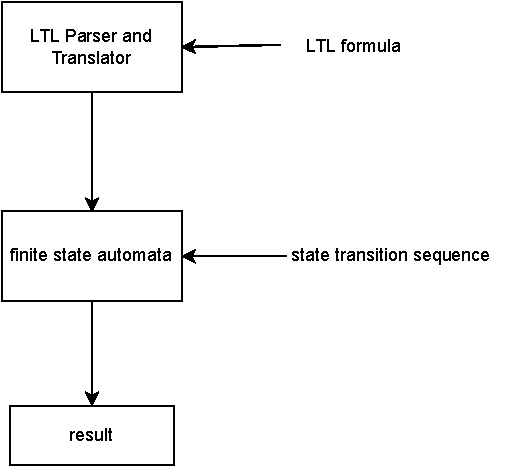
\includegraphics[width=0.5\textwidth]{./figs/translator}
\bicaption{LTL检查器}{LTL Checker}
\label{fig:translator}
\end{figure*}

以下为基于该框架的LTL检查算法:
\begin{algorithm} % This algorithm can also be used
\caption{LTL检查器}\label{checker}
\begin{algorithmic}[1]
\STATE 输入:$(\rho, o)$
\STATE $l \gets getLTL(o)$
\STATE $\alpha \gets transform(l)$ \COMMENT{将LTL转换为状态机}
\FOR{$i \leftarrow 0, len(\rho)-1$}
  \STATE $s \gets si(\rho, i)$
  \IF {$\alpha$ 在 $s$状态下可转移}
    \STATE $\alpha.transit(s)$
    \ELSE
    \STATE $trigger(o)$
  \ENDIF
\ENDFOR
\IF {$o$ 为实现型目标且$\alpha$为最终状态}
  \STATE $o.achieved()$
\ENDIF
\end{algorithmic}
\end{algorithm}
该检查器的输入参数有两个:游程$\rho$和一个LTL对象$o$。
%
% @TODO: line number ref.
检查器首先得到LTL公式并将其转化为状态机。然后$\rho$中的每个状态都由状态机迭代处理并根据每个环境状态进行状态机的状态转移\footnote{注意,环境状态与状态机中的状态是两个不同的概念。};如果状态机可在当前环境状态下进行转换,则应用该转换。否则,状态机不接收当前环境状态,其相应LTL对象被触发。对于维持型目标,出发意味着维持条件不满足,智能体此时应执行相关修复计划;对于norm,触发意味着norm被触发且智能体收到相应的价值;最后,如果该LTL公式对应一个实现型目标,并且状态机处于其最终状态(Final State),那么该目标被视为已实现。

算法\ref{trigger}所示的触发函数用于对触发LTL对象的相应操作。
\begin{algorithm} % This algorithm can also be used
\caption{触发函数}\label{trigger}
\begin{algorithmic}[1]
\STATE 输入:$(o)$

\IF {$o$ 为维持型目标且无相关计划在执行}
\STATE 选择并执行一个相关计划
\ELSE
\IF {$o$为norm}
\STATE 获得价值 $o.val$
\ENDIF
\ENDIF

\end{algorithmic}
\end{algorithm}

在描述对\SA 方法的修改之前,本节首先描述智能体的初始设定以及骑在执行期间的内部状态转换规则:假设智能体在开始执行时被分配了一组需要满足的LTL公式,在正式执行之前,智能体首先将每个LTL公式转化为状态机(状态机为智能体内部状态的一部分);在智能体执行过程中,每次更新智能体信念集合时,所有状态机都会根据智能体当前对环境的认知进行状态转移;如果在当前认知下,状态机中可由可应用的状态转移规则,则按照算法\ref{checker}所述触发其相关操作。

\subsection{对\SA 方法的拓展}
为了支持LTL表示形式下的意图调度,\SAT 拓展了\SA 算法中的扩展与模拟阶段,具体拓展如下:
\paragraph{对扩展阶段的拓展}
% Reactive
在扩展阶段,\SAT 首先检查某个选中的叶子节点$n_s$状态下每一个可执行动作$a_i$,若$a_i$所引发的(状态机的)状态转移不会使得智能体获得负收益,则直接生成一个新的节点对应于执行$a_i$的结果,并作为$N_s$的一个孩子节点。若$a_i$会引发负收益,则首先进行如下检查:检查$a_i$所对应的状态机$m_i$,若$m_i$可获得的最终的价值$V_i$大于当前执行$m_i$相关动作所受到的总惩罚值$P_i$(包括执行$a_i$的惩罚值),则生成一个新节点对应于执行$a_i$的结果。相反,若$m_i$可获得的最终价值$V_i$小于当前执行$m_i$相关动作所受到的总惩罚值$P_i$,则不生成新的节点。
%
当所有可执行动作$a_i$都会造成$P_i > V_i$时,则不会有新的节点生成。该情况下智能体会暂停其执行。
%
在\SAT 中,每个节点记录的信息除智能体意图、环境状态外,还记录了执行过程中所收到的总价值(收益值以及惩罚值)和每个状态机单独得到的价值。

\paragraph{对模拟阶段的拓展}
在模拟阶段,\SAT 和\SA 一样,随机选择实现目标过程中可执行的动作执行。当某个可执行动作$a_i$造成状态机的状态转移并获得负收益时时,进行如下检查:检查$a_i$对应的状态机$m_i$,若可获得的最终的价值$V_i$大于当前执行$m_i$相关动作所受到的总惩罚值$P_i$(包括执行$a_i$的惩罚值),则禁止该动作的执行。相反,若$m_i$可获得的最终价值$V_i$小于当前执行$m_i$相关动作所受到的总惩罚值$P_i$,则直接执行。

当以下三个条件中的任意一个满足时,模拟阶段即停止:
\begin{enumerate}
  \item 所有状态机都处于最终状态。
  \item 并非所有状态机都处于最终状态,但是智能体无法执行相关动作将其带入最终状态。
  \item 所有的可执行动作$a_i$都会导致$m_i$可获得的最终价值$V_i$小于当前执行$m_i$相关动作所受到的总惩罚值$P_i$。
\end{enumerate}

\section{实验}
本章的实验场景与上一章类似,基于火星探测器的模拟场景。
和前两章不同的是,本章假设地图上有一些形状不同的斜坡,每个斜坡都有两条边:高地边和低地边。特工可以安全地从高地移动到低地,但从低地移动到高地是危险的。从低地移动到高地会触发违规行为,智能体将受到一定的处罚(见图\ref{fig:marsrover})。
在本章中,实验场景有两个:斜坡形状与位置随机分布的复杂地形环境与斜坡位置固定与中间的简单地形环境。

% measring the agent performance
本章根据三个标准来衡量火星车代理的性能:实现目标的收益、电池消耗量和受到的惩罚。具体来说,本章通过一评估函数来衡量代理的性能:$\frac{\sum_{g \in G} reward(g) - c\sum_{n \in N} penalty(n)}{consumption}$,其中$G$是包含所有目标的集合,$reward(g)$是实现目标$g$的奖励,$c$是一个常数,用于控制惩罚的重要性,$N$包含所有违反norm的记录,$penalty(n)$是违反$n$的惩罚值;最后,$consumption$是电池的总消耗量。该评估函数决定了智能体的总体效用。

在以下实验中,每个违反norm的惩罚值为1,$c$设定为1;对于$G$中的每个目标$g$,$reward(g)$的值为1。

本文将\SAN 与Duff等人\cite{DBLP:conf/atal/DuffHT06}提出的PMG(本章对RMG也进行了实验,其作为基准以衡量其他方法的性能)和Meneguzzi等人\cite{DBLP:journals/eaai/MeneguzziROVL15}提出的v-BDI进行比较。PMG和v-BDI算法分别在第\ref{mg}章和第\ref{norm}章有所解释,在此不再赘述。
在接下来的实验中,\SAN 的价值函数与v-BDI相同,都设定为为$\frac{\sum_{g \in G} reward(g) - c\sum_{n \in N} penalty(n)}{consumption}$。\SAN 算法设定为执行100次迭代($\alpha = 100$),每次迭代执行10次的模拟($\beta = 10$)。

\subsection{复杂地形实验}
在复杂的地形场景中,环境中有许多形状不同的短斜坡。确切的地形设置如图\ref{fig:complex}所示。
\begin{figure}[H]
\centering
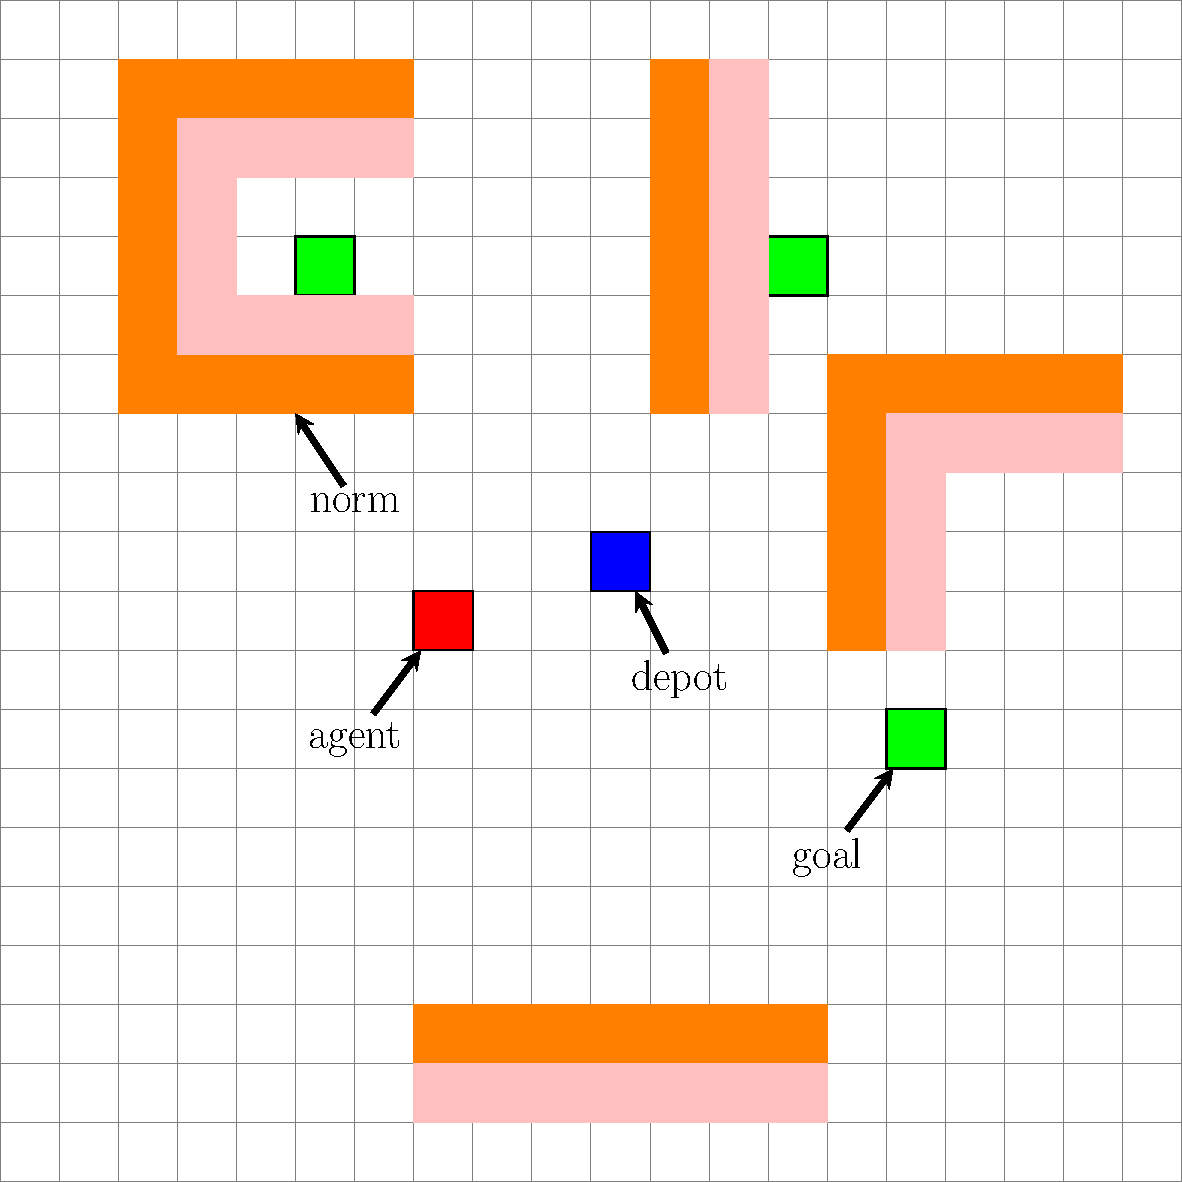
\includegraphics[scale=0.5]{MR_complex_norm_example.pdf}
\captionsetup{justification=centering}
\bicaption{复杂地形场景}{Complex terrain scenario}
\label{fig:complex}
\end{figure}

\paragraph{静态场景}
本实验考虑了智能体在静态环境中的执行的情景,在该场景中,所有目标在初始时给定。在不同的容量设置中,将要实现的目标数量从1个改变到15个不等。结果如图\ref{fig:static_complex}所示。

\begin{figure}[H]
\centering
\begin{subfigure}{.32\textwidth}
  \centering
  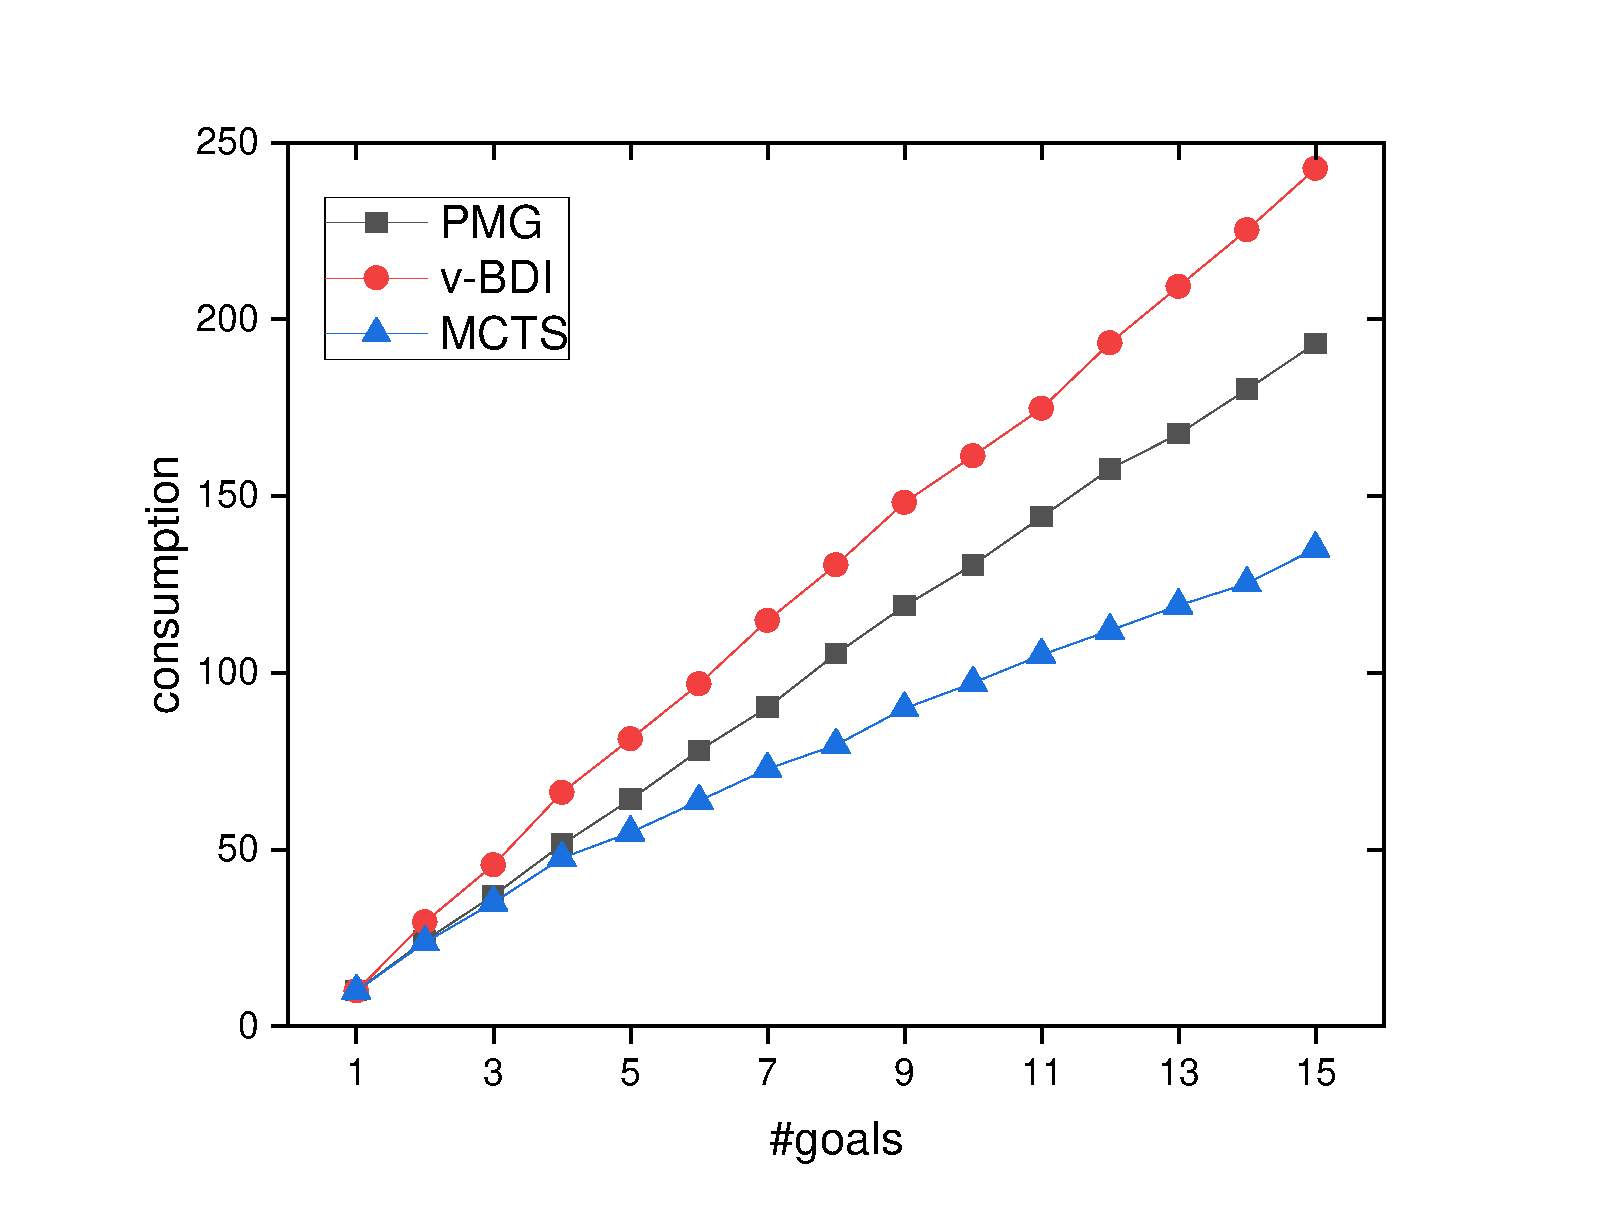
\includegraphics[scale=0.2]{gX_consY_fixCap40_complex}
  \caption{40容量}
  \captionsetup{justification=centering}
\end{subfigure}
\begin{subfigure}{.32\textwidth}
  \centering
  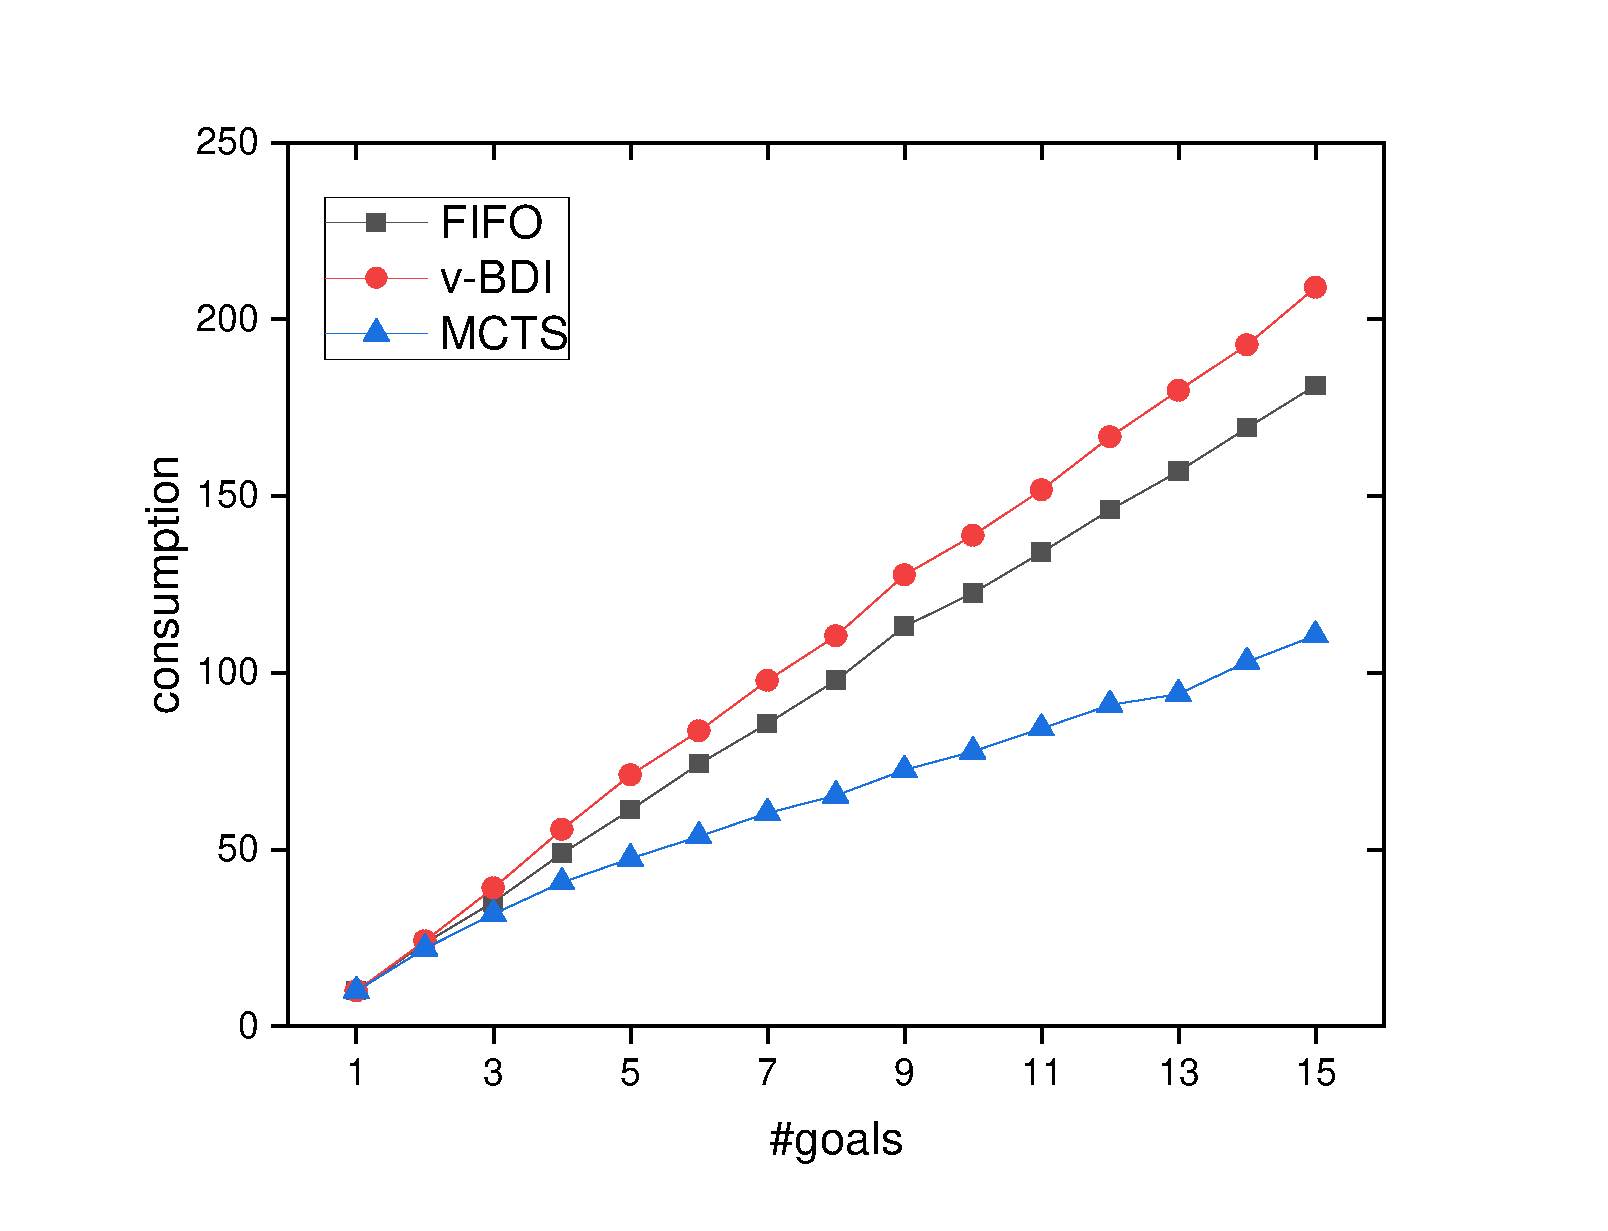
\includegraphics[scale=0.2]{gX_consY_fixCap60_complex}
  \caption{60容量}
  \captionsetup{justification=centering}
\end{subfigure}
\begin{subfigure}{.32\textwidth}
  \centering
  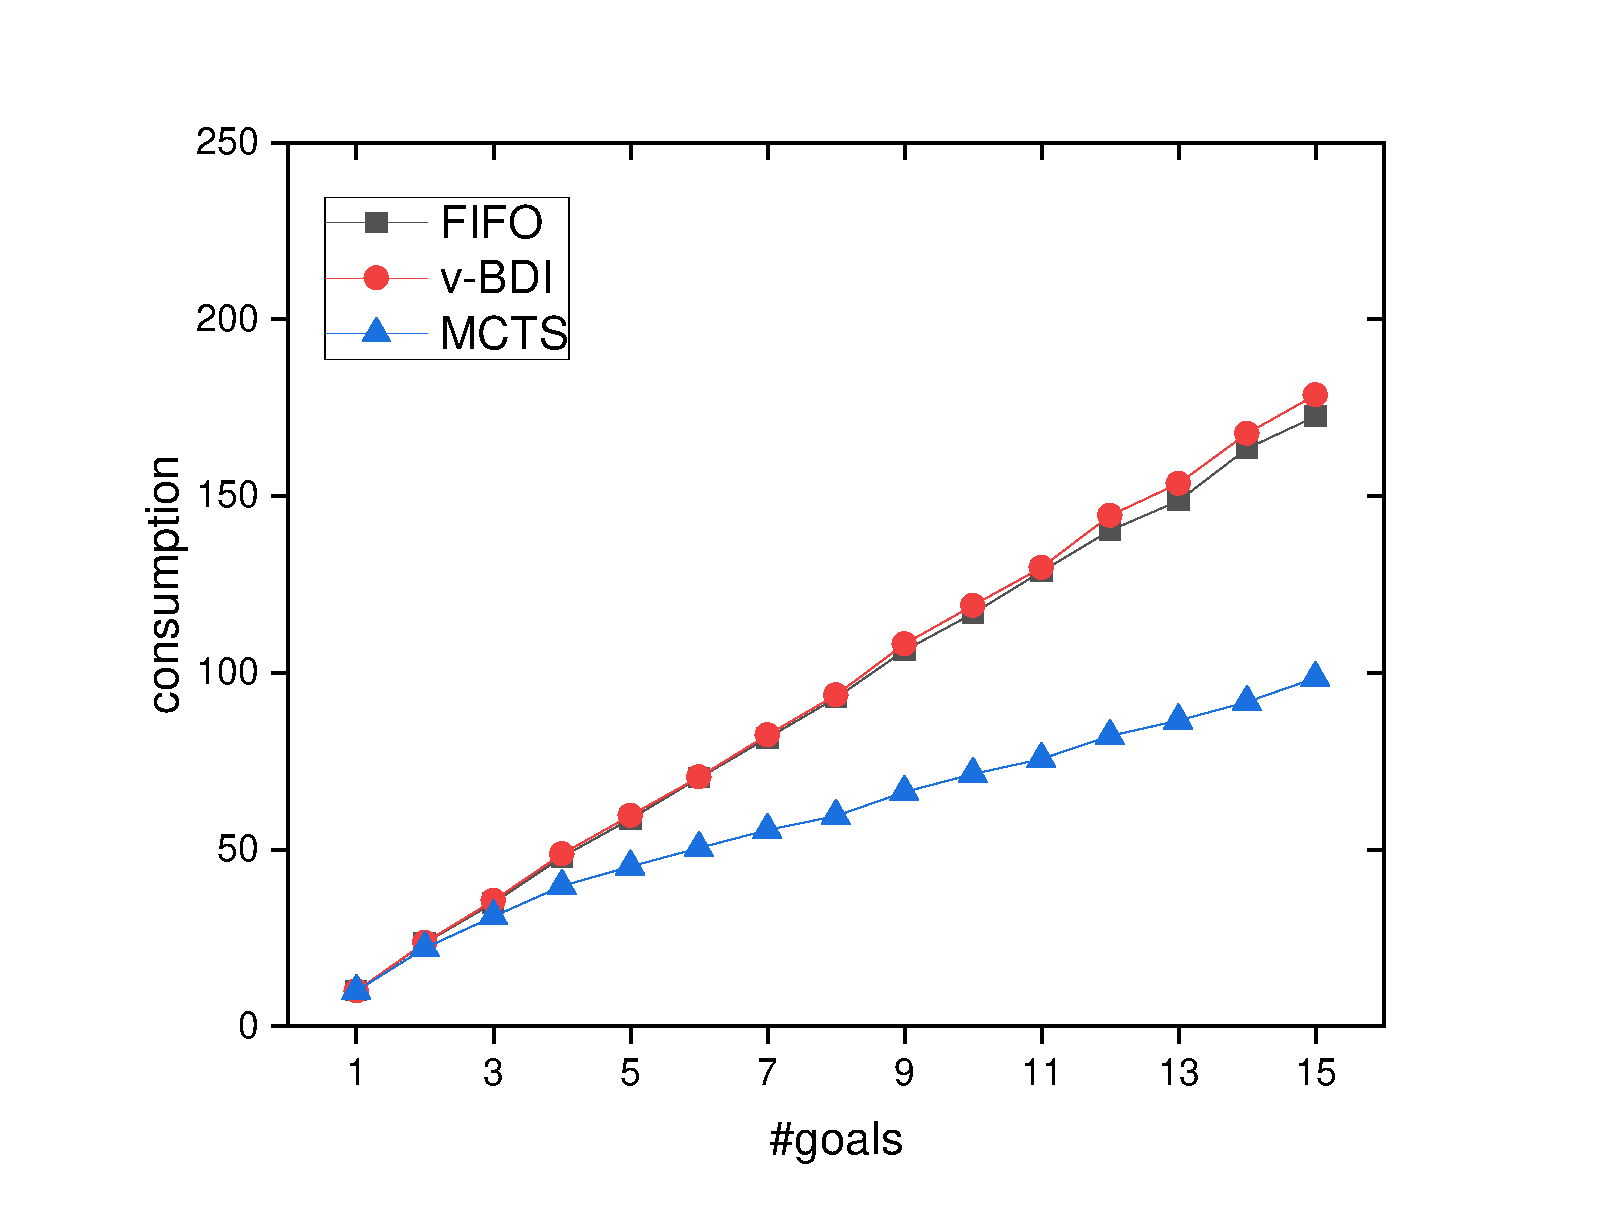
\includegraphics[scale=0.2]{gX_consY_fixCap140_complex}
  \caption{140容量}
  \captionsetup{justification=centering}
\end{subfigure}
\begin{subfigure}{.32\textwidth}
  \centering
  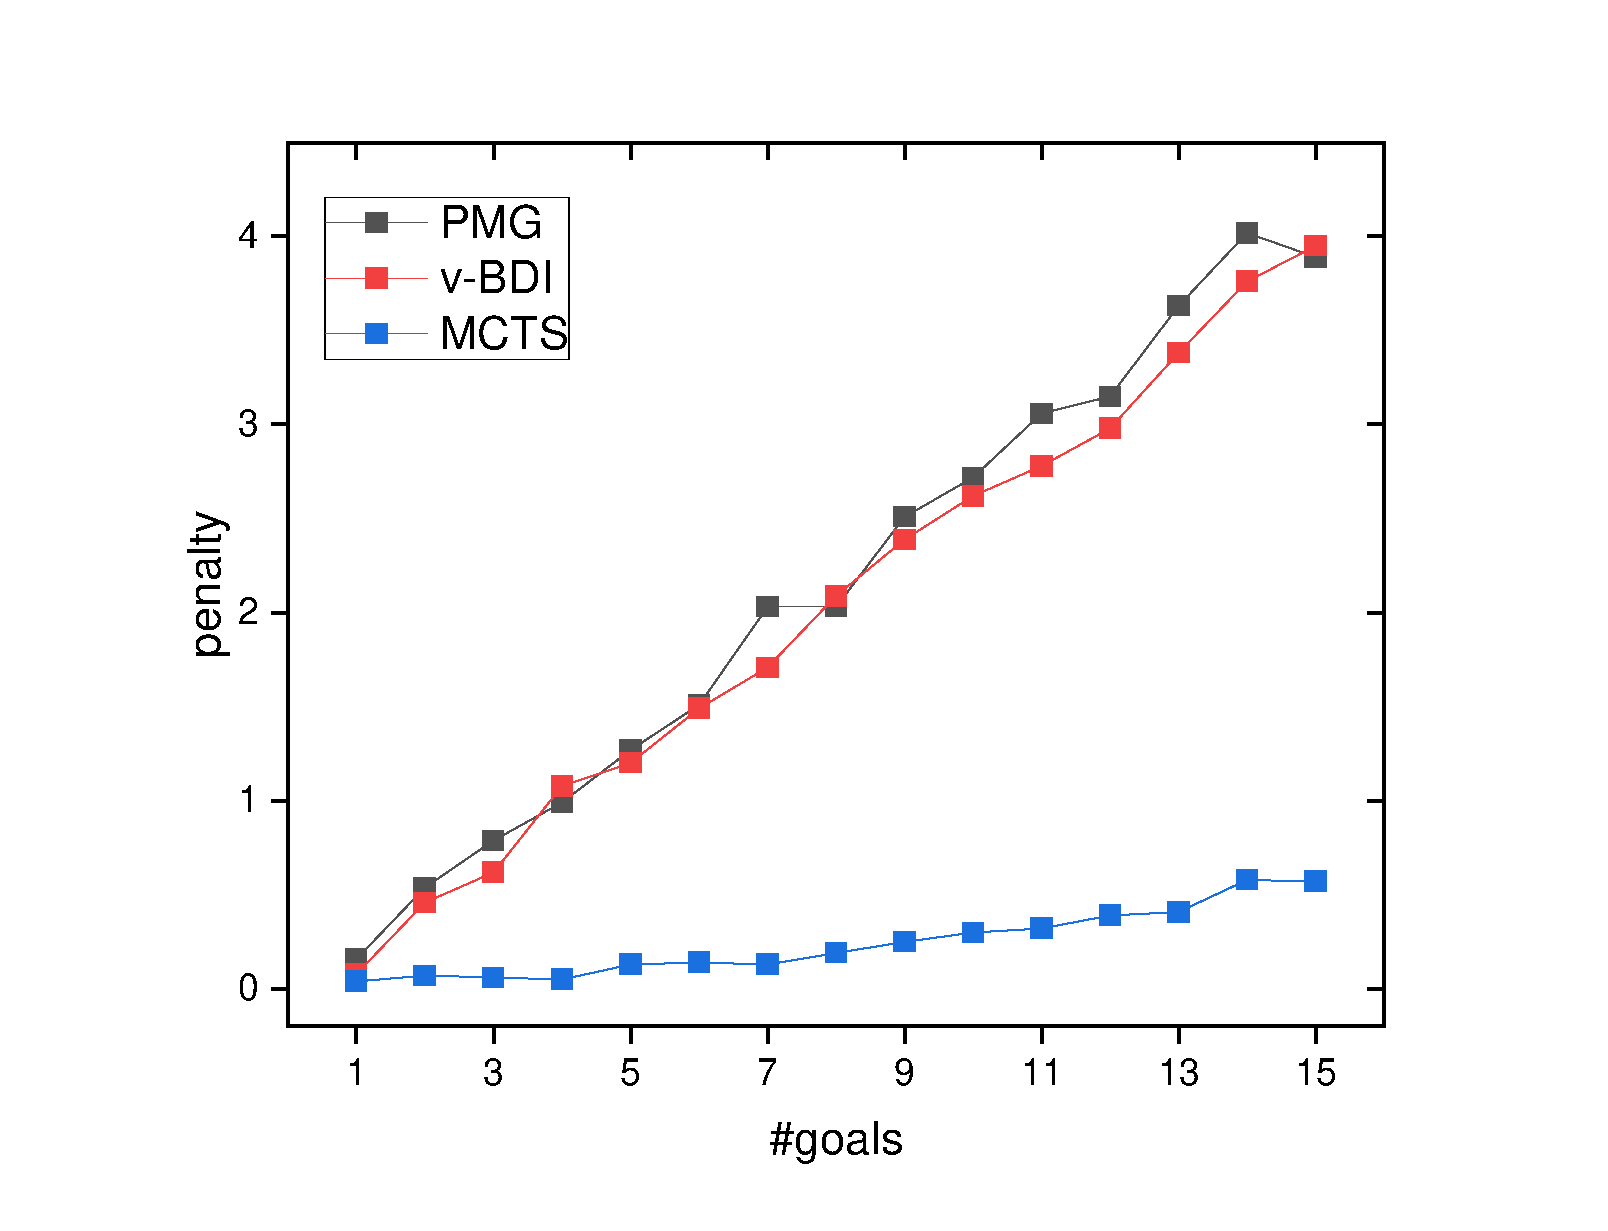
\includegraphics[scale=0.2]{gX_pY_fixCap40_complex}
  \caption{40容量}
  \captionsetup{justification=centering}
\end{subfigure}
\begin{subfigure}{.32\textwidth}
  \centering
  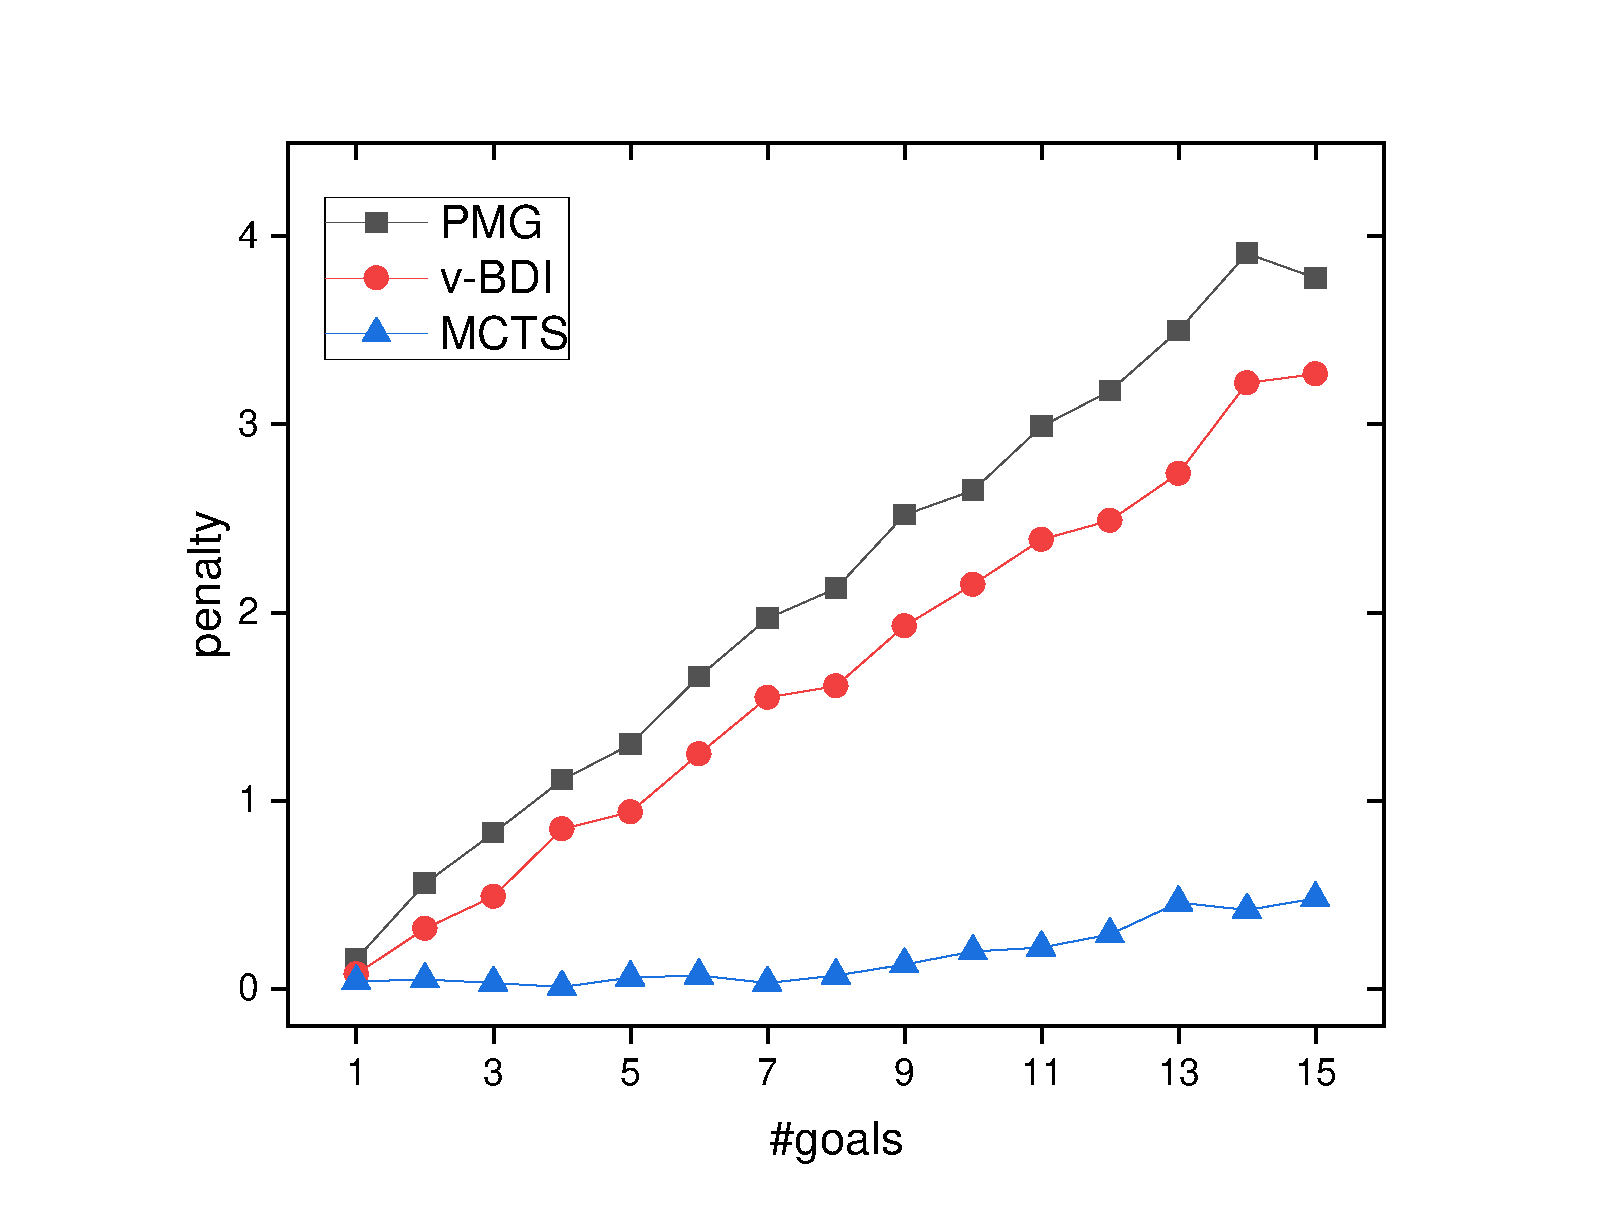
\includegraphics[scale=0.2]{gX_pY_fixCap60_complex}
  \caption{60容量}
  \captionsetup{justification=centering}
\end{subfigure}
\begin{subfigure}{.32\textwidth}
  \centering
  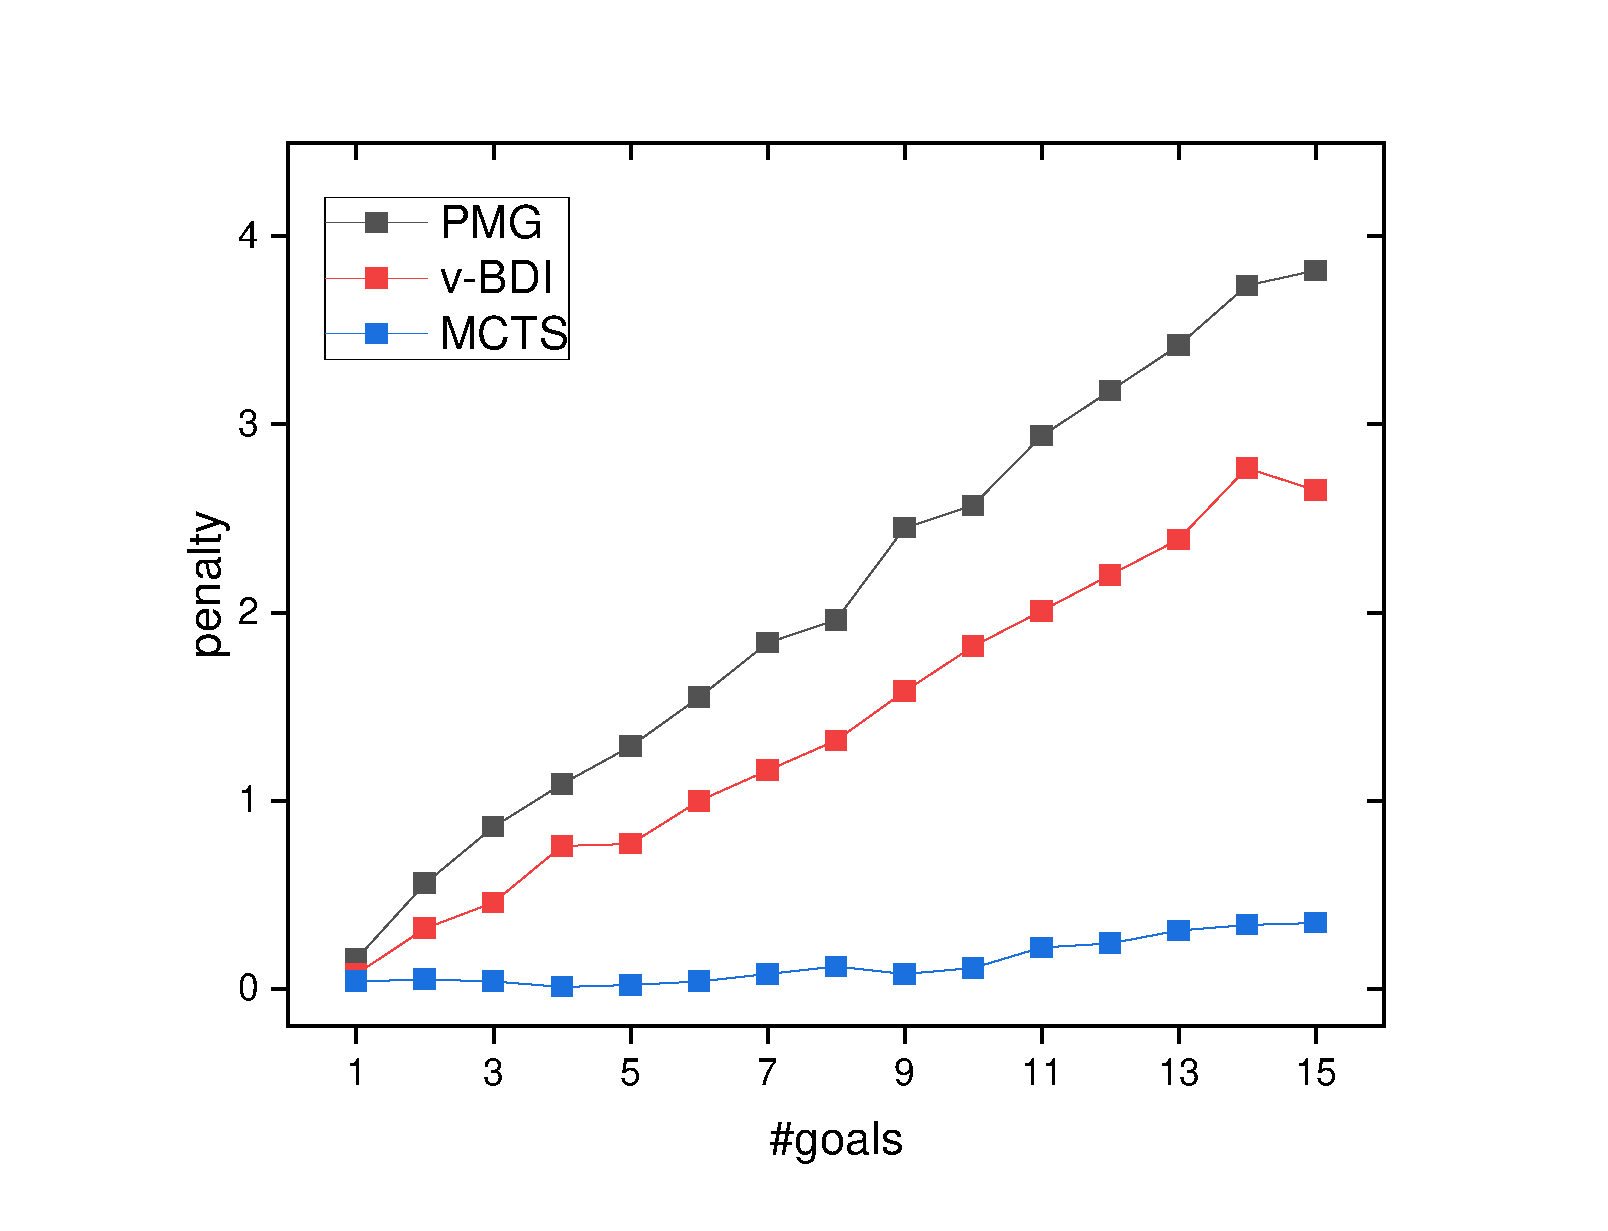
\includegraphics[scale=0.2]{gX_pY_fixCap140_complex}
  \caption{140容量}
  \captionsetup{justification=centering}
\end{subfigure}
\begin{subfigure}{.32\textwidth}
  \centering
  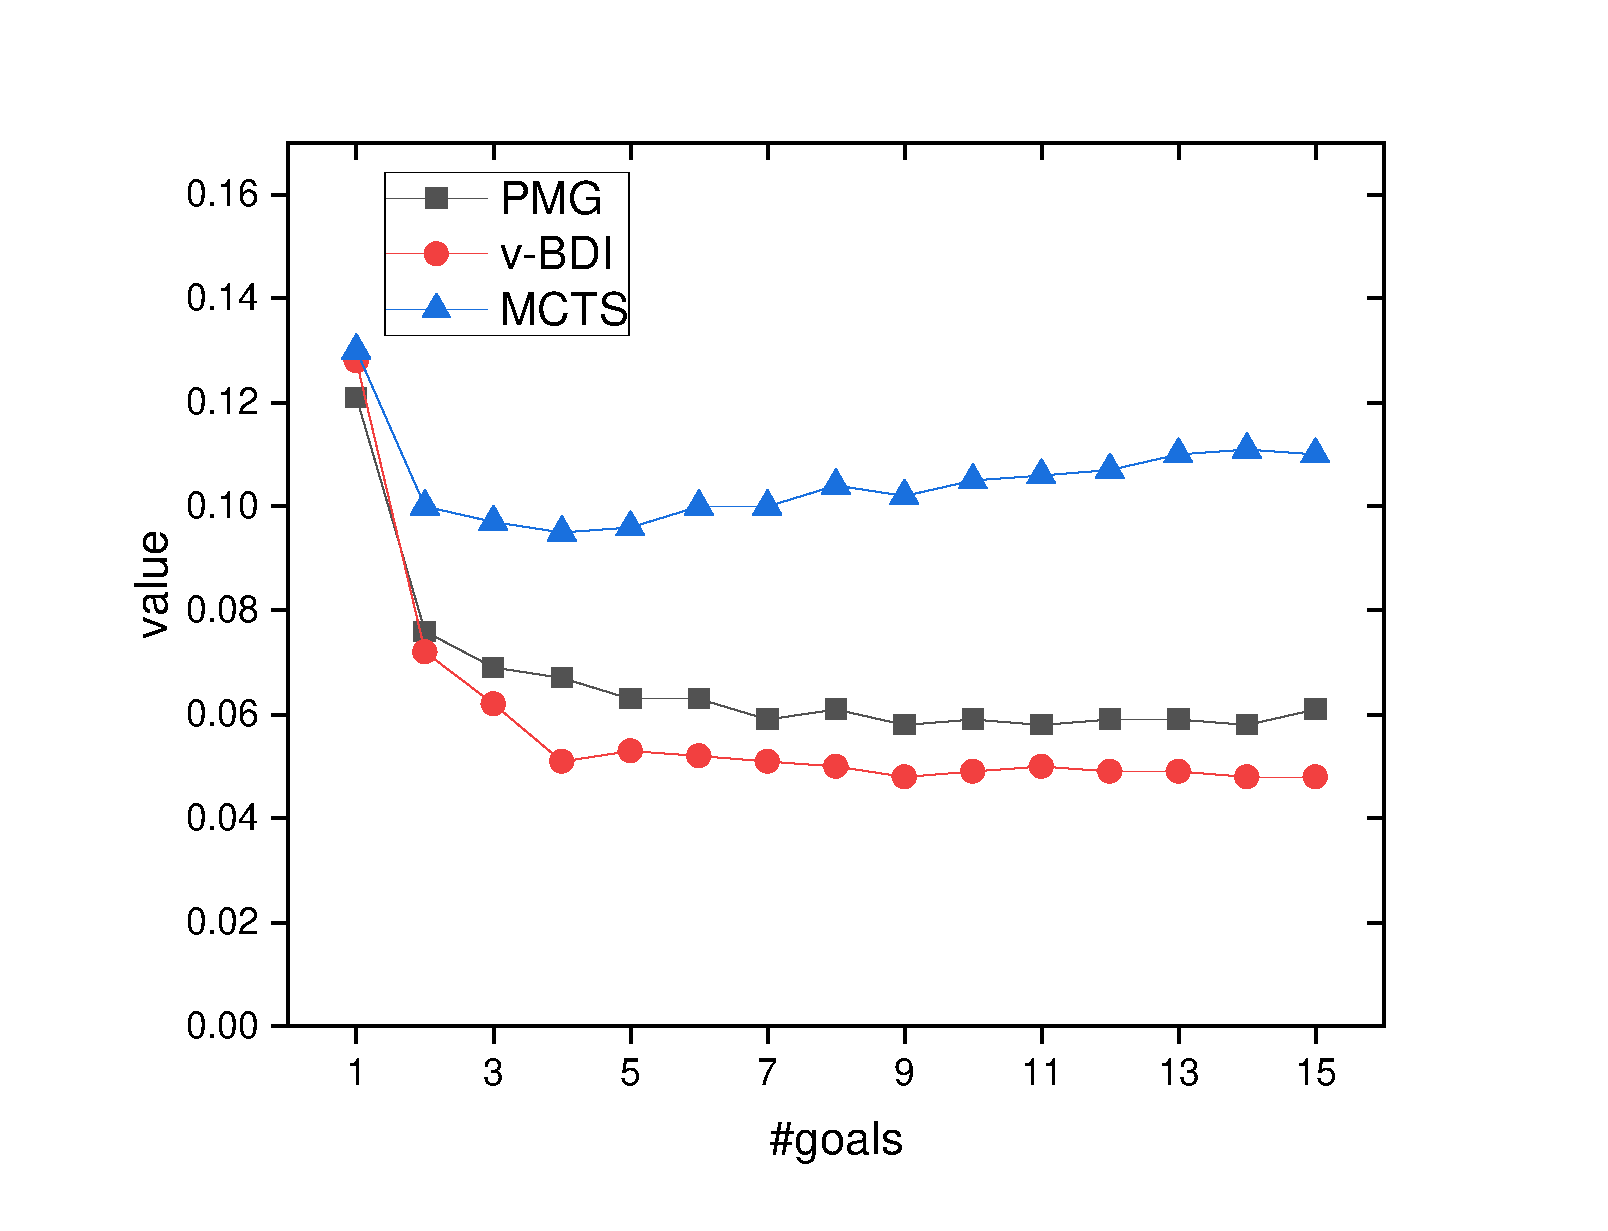
\includegraphics[scale=0.2]{gX_vY_fixCap40_complex}
  \caption{40容量}
  \captionsetup{justification=centering}
\end{subfigure}
\begin{subfigure}{.32\textwidth}
  \centering
  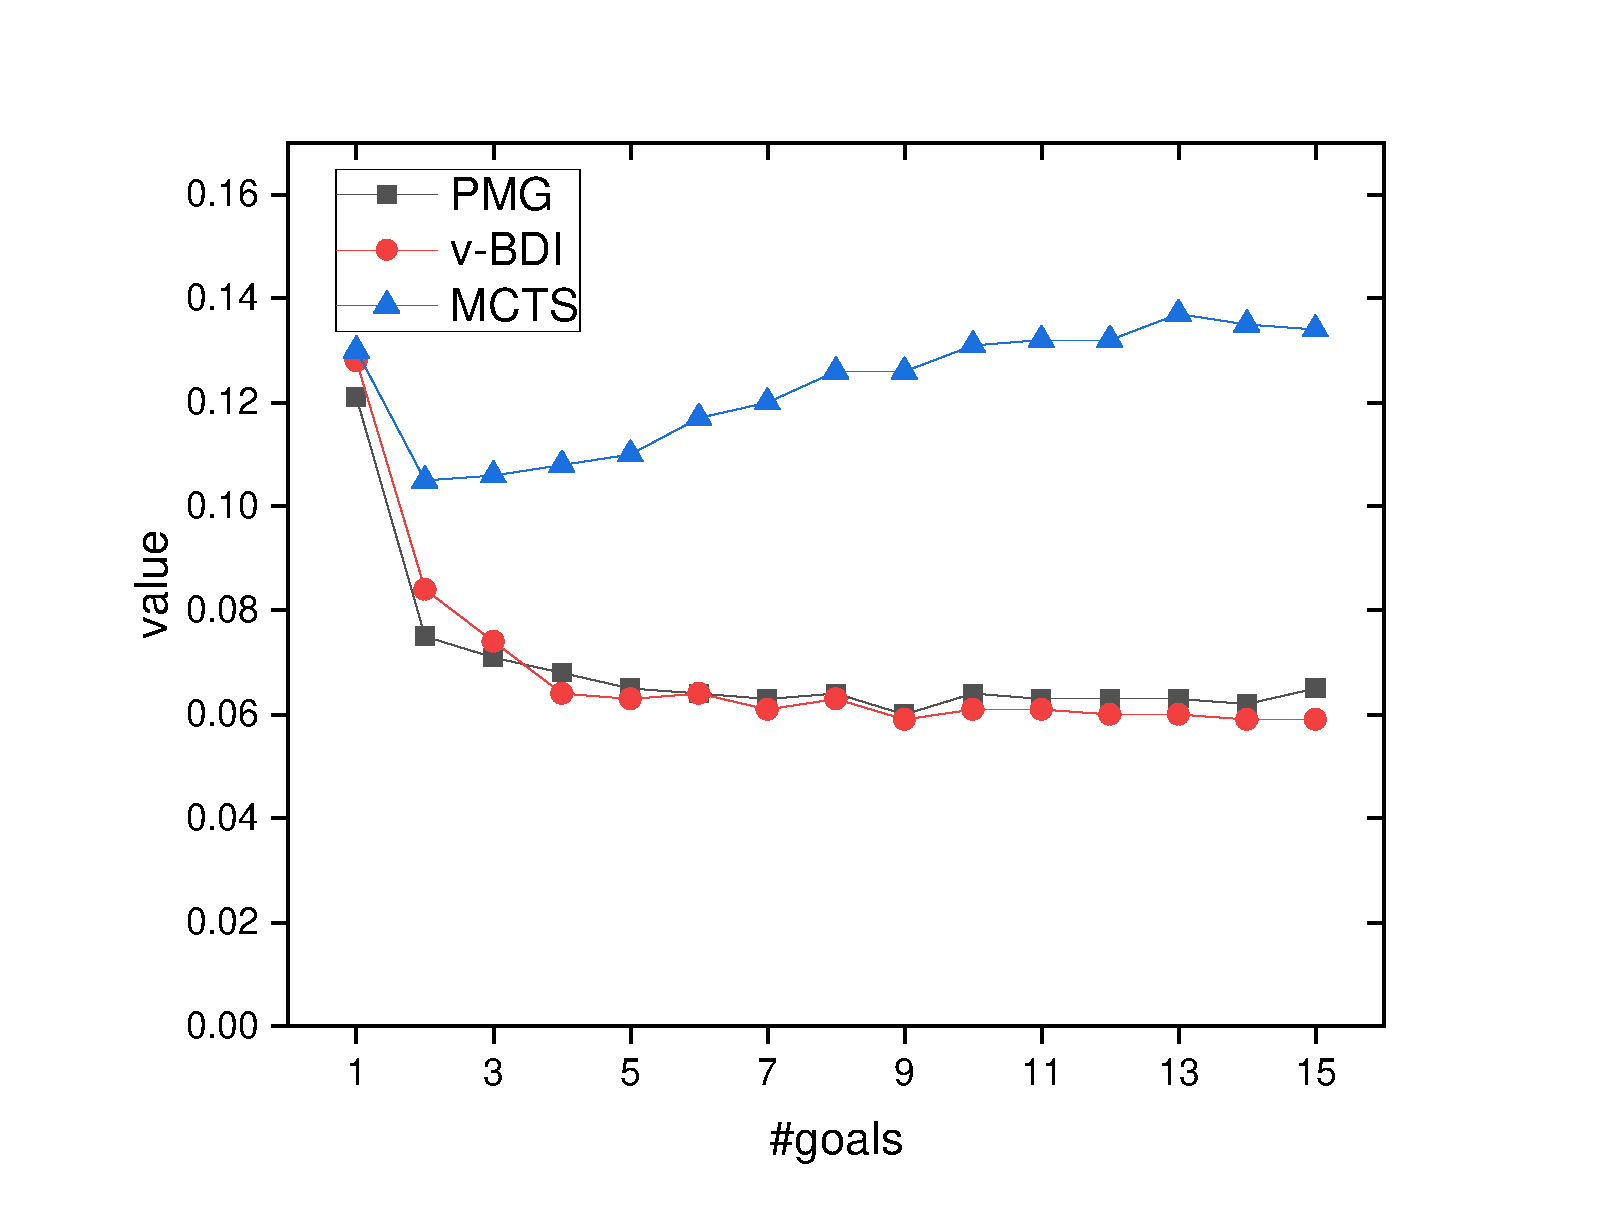
\includegraphics[scale=0.2]{gX_vY_fixCap60_complex}
  \caption{60容量}
  \captionsetup{justification=centering}
\end{subfigure}
\begin{subfigure}{.32\textwidth}
  \centering
  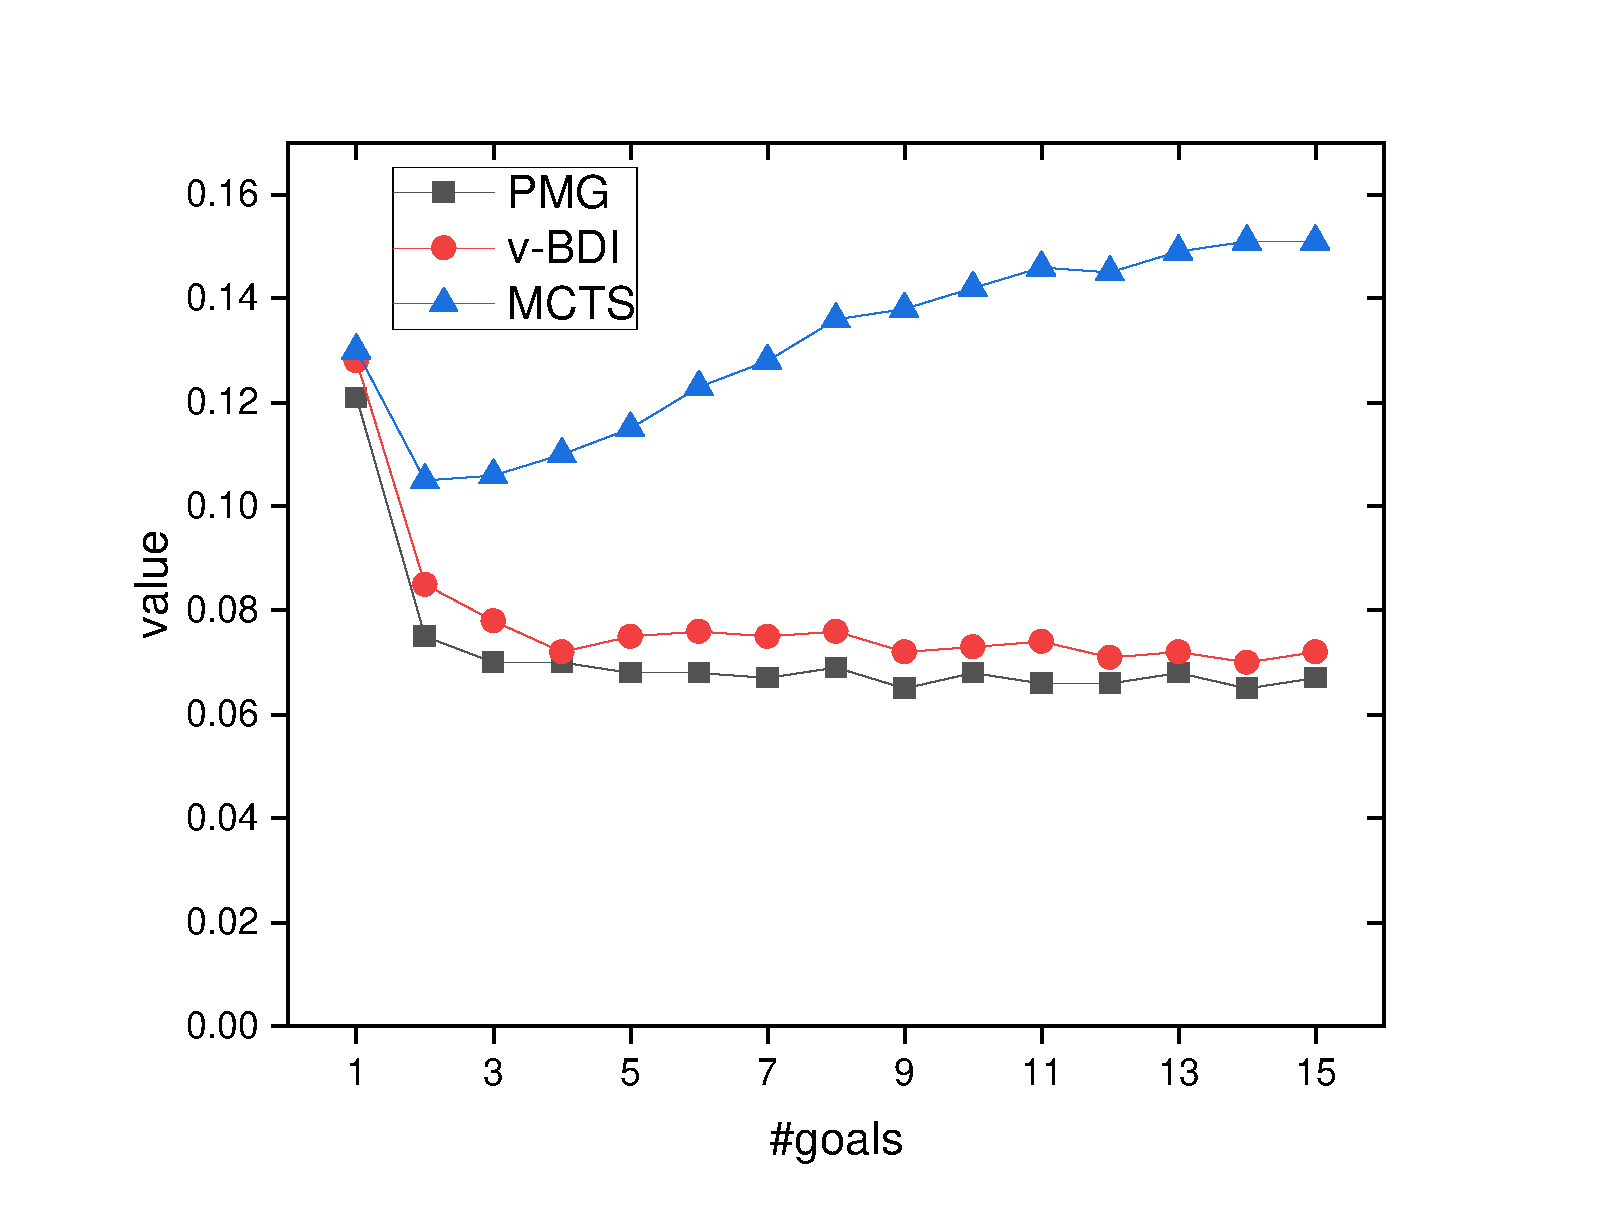
\includegraphics[scale=0.2]{gX_vY_fixCap140_complex}
  \caption{140容量}
  \captionsetup{justification=centering}
\end{subfigure}
\captionsetup{justification=centering}
\bicaption{复杂地形下的静态场景实验结果}{Experiment results in static complex terrain scenario}
\label{fig:static_complex}
\end{figure}
从图中可以看出,在电池消耗方面,PMG比v-BDI具有更好的性能。这是因为PMG可以在追求目标之前主动估计电池消耗量。如果实现下一个目标将触发维护目标,智能体将首先前往停车场充电,然后追求下一个目的。这节省了许多执行步骤,从而减少了运行过程中的电池消耗。与v-BDI和PMG相比,MCTS消耗的电池要少得多,因为它不仅可以预测执行过程中可能违反维持条件的情况,还可以利用不同意图之间可能的协同作用(即智能体可以将不同意图的相同动作合并以节省时间和资源)。
另一方面,随着容量变大,所有方法的电池消耗都会增加。当容量较大时,v-BDI和PMG之间的差异较小,因为增加的容量逐渐超过了在不充电的情况下实现所有目标的需要。容量越大,对智能体的帮助就越小。

在惩罚方面,v-BDI比PMG具有更好的性能,因为它可以选择导致更少惩罚的计划,而PMG不考虑norm,所有违反规范的事件都被忽略。MCTS受到的惩罚最少,因为它可以积极避免违反规范。此外,MCTS可以将相同的动作合并到不同的意图中,缩短地图上的旅行距离,从而减少违反规范的可能性。
当容量较低时,PMG和v-BDI的惩罚非常接近。原因是PMG的行进距离比v-BDI短;更短的旅行距离有助于减少违反规范的次数。因此,即使PMG根本不考虑范数,与v-BDI相比,它仍然具有类似的性能。然而,随着容量的增加,主动维护目标的好处变得不那么突出,v-BDI的优势也更加明显。最后,与其他方法相比,MCTS仍然具有显著优势。

就整体效用而言,PMG和v-BDI的性能与预期一致。然而,随着目标数量从1个增加到2个,MCTS的绩效明显下降,但当目标数量变多时,总价值有所提高。这是因为,当目标数量较少时,意图之间的协同作用很难发挥,导致总体效用较低;然而,当目标数量变大时,MCTS可以更好地利用意图之间的协同效应,因此,利用协同效应的收益可以超过增加惩罚的危害,从而产生更好的效用价值。
当容量较低时,PMG比v-BDI具有更好的性能。这表明,主动维持型目标的好处超过了在这种情况下缺乏规范性考虑的缺点。然而,当容量较大时,v-BDI的性能优于PMG,因为主动维持型目标的优势变得不那么突出,v-BDI的优势更加明显。

\paragraph{动态场景}
为了研究方法在动态环境中的性能,本实验假设并非所有的顶层目标都是初始给定的。
相反,随着时间的推移,这些目标被分配给了智能体。以下的实验假设最初给出两个目标(如果顶层目标的总数为1,那么在场景开始时只发布一个目标),其余目标每$n$步分配一次(假设每个动作需要1步才能执行)。具体实验结果如图\ref{fig:dynamic_complex}所示。

在动态设置中,MCTS仍然优于其他方法。然而,使用MCTS的好处随着时间间隔的增加而减少。原因是间隔越长智能体并行的目标就越少,这使得MCTS更难利用不同意图之间的协同作用。当时间间隔设置为15时,在大多数情况下,智能体只有一个目标。因此,MCTS的性能与其他方法非常接近。然而,当容量较大(140)时,即使MCTS和v-BDI的油耗接近,MCTS仍然比v-BDI受到更少的处罚。这表明MCTS在避免违反规范方面比v-BDI更有效。这是因为MCTS可以预测更长的执行路径(因为它可以构建深度搜索树),而v-BDI只考虑即时计划。因此,MCTS能够实现更高的全局最优,而v-BDI只能实现局部最优。
\begin{figure}[H]
\centering
\begin{subfigure}{.32\textwidth}
  \centering
  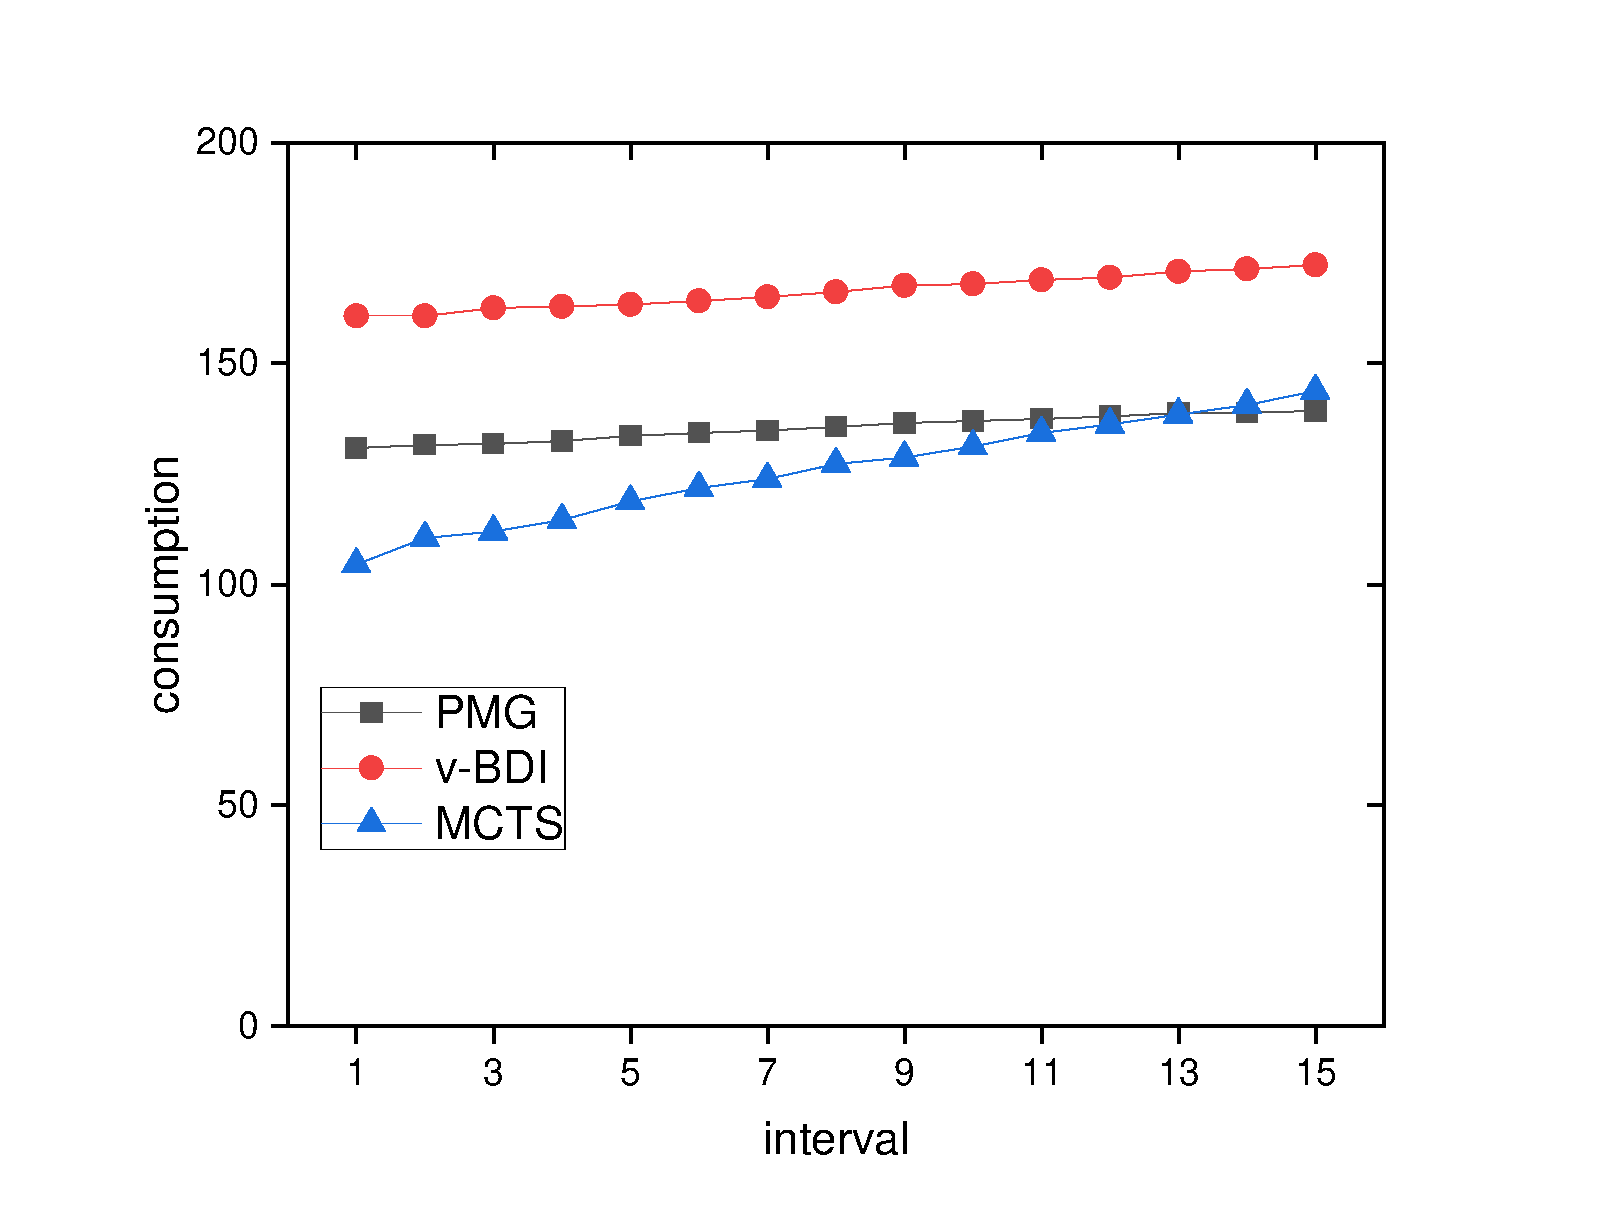
\includegraphics[scale=0.2]{inX_consY_fixCap40_complex}
  \caption{40容量}
  \captionsetup{justification=centering}
\end{subfigure}
\begin{subfigure}{.32\textwidth}
  \centering
  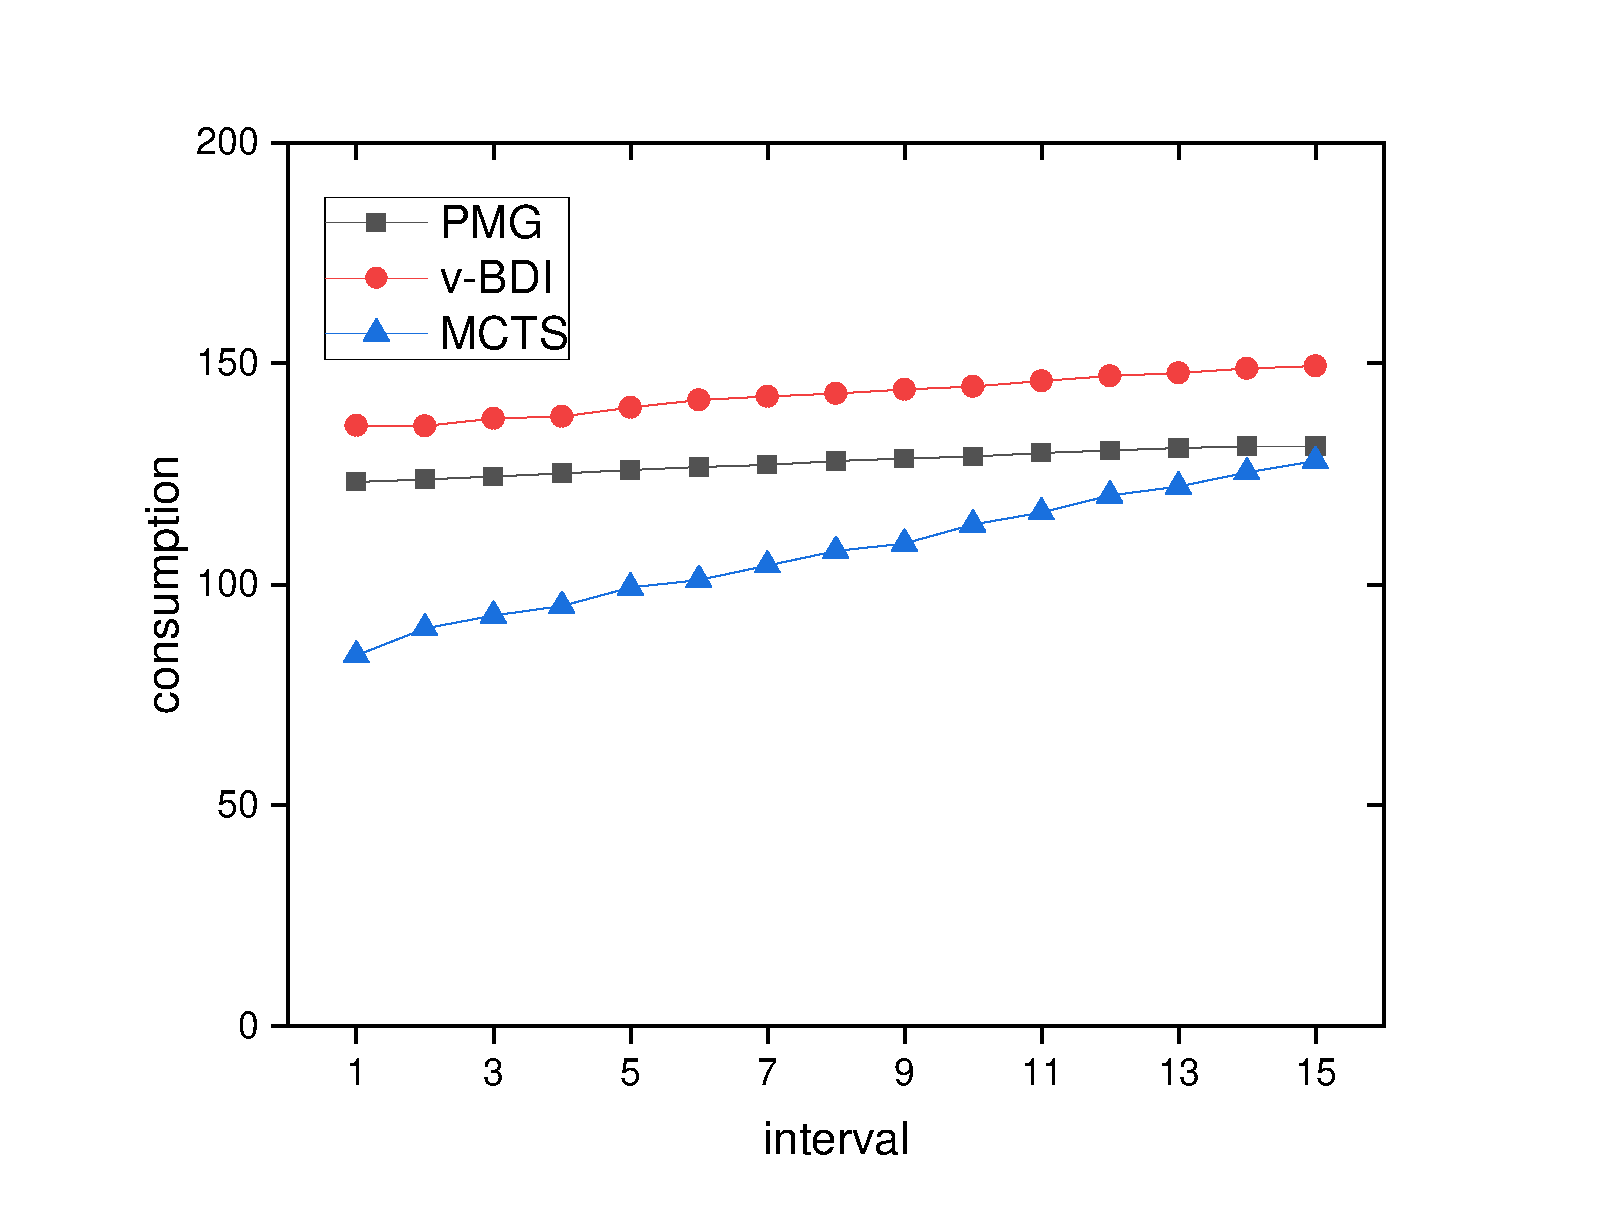
\includegraphics[scale=0.2]{inX_consY_fixCap60_complex}
  \caption{60容量}
  \captionsetup{justification=centering}
\end{subfigure}
\begin{subfigure}{.32\textwidth}
  \centering
  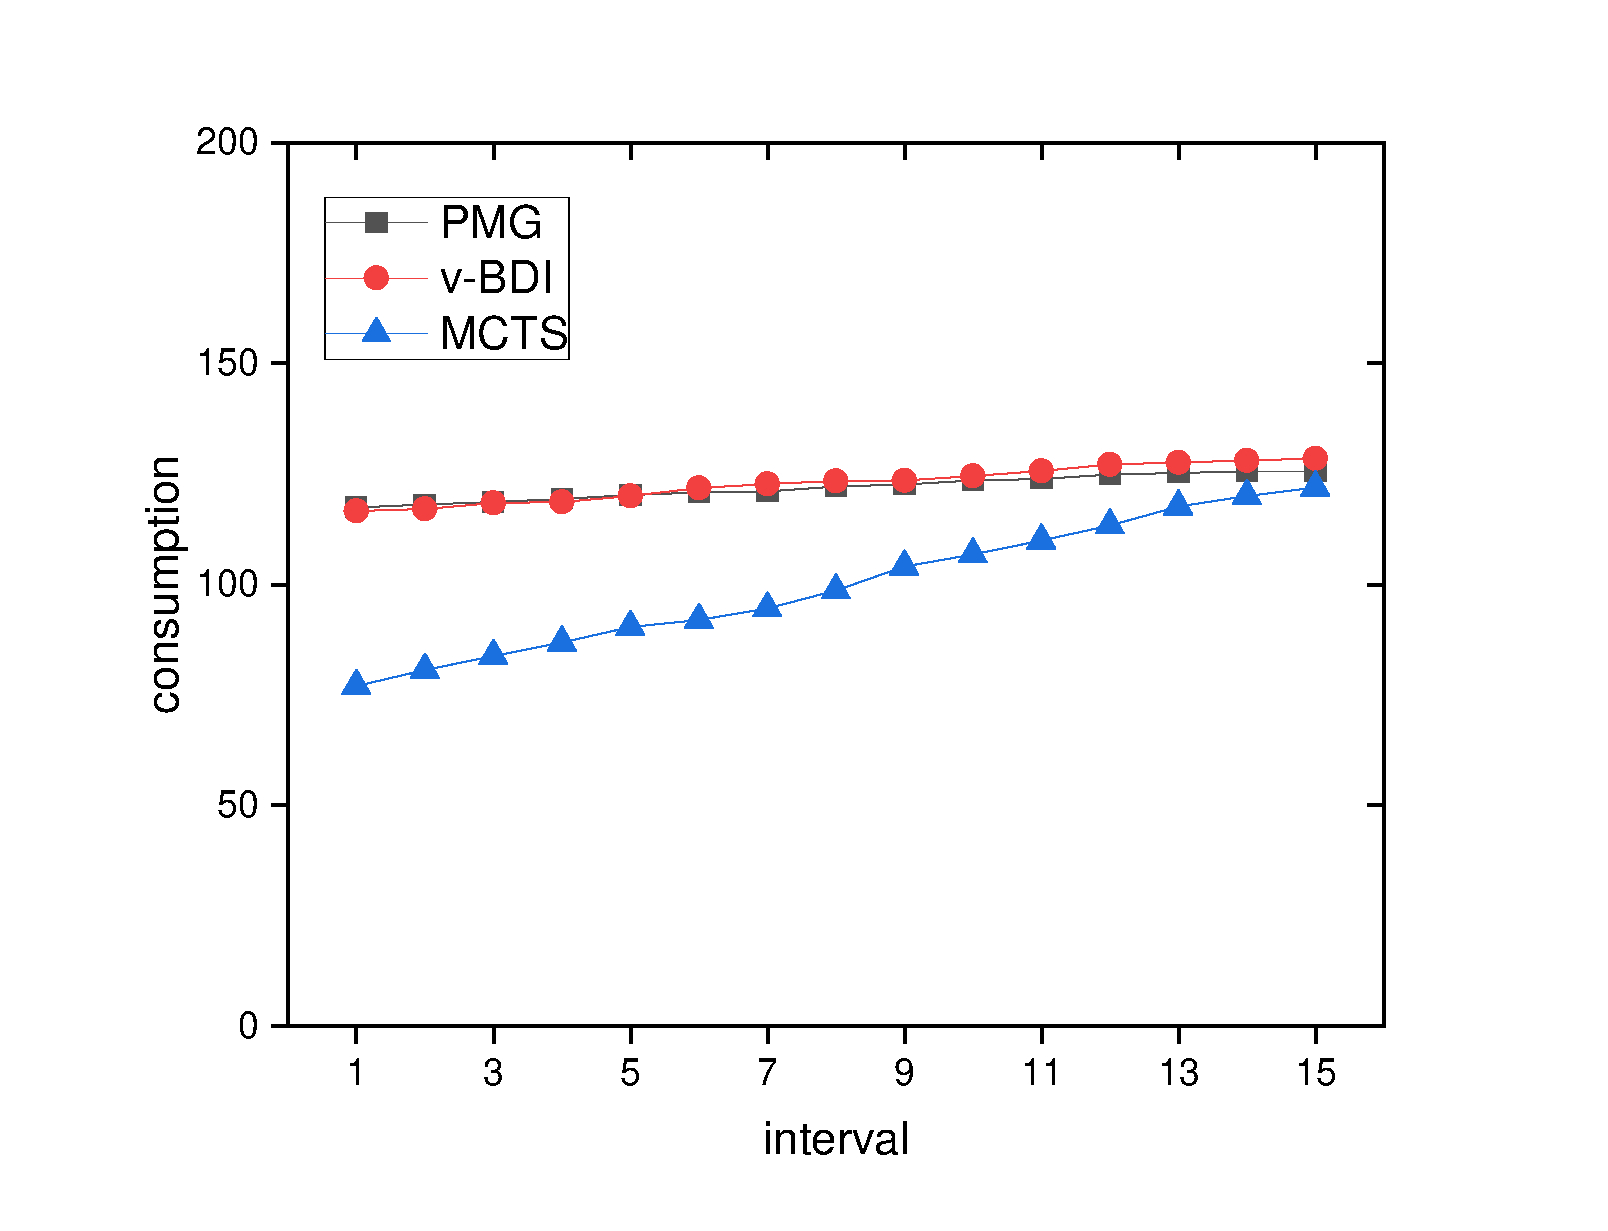
\includegraphics[scale=0.2]{inX_consY_fixCap140_complex}
  \caption{140容量}
  \captionsetup{justification=centering}
\end{subfigure}
\begin{subfigure}{.32\textwidth}
  \centering
  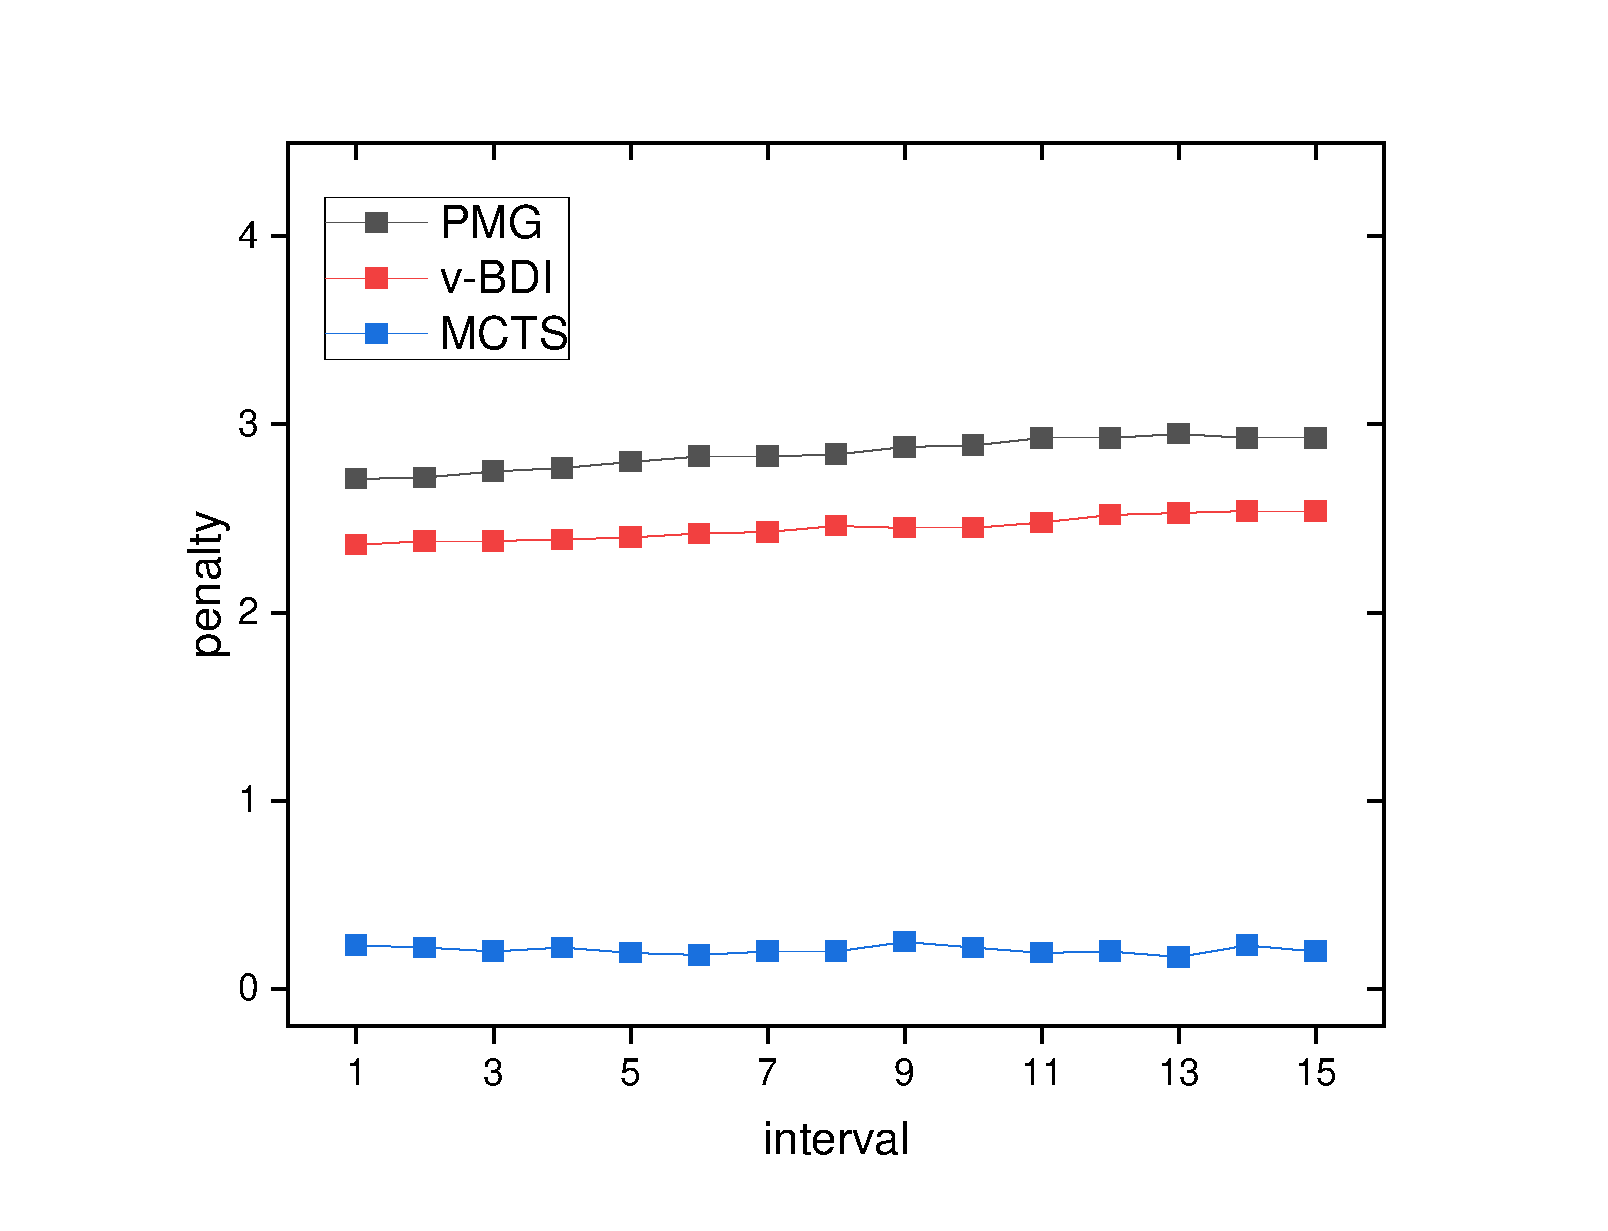
\includegraphics[scale=0.2]{inX_pY_fixCap40_complex}
  \caption{40容量}
  \captionsetup{justification=centering}
\end{subfigure}
\begin{subfigure}{.32\textwidth}
  \centering
  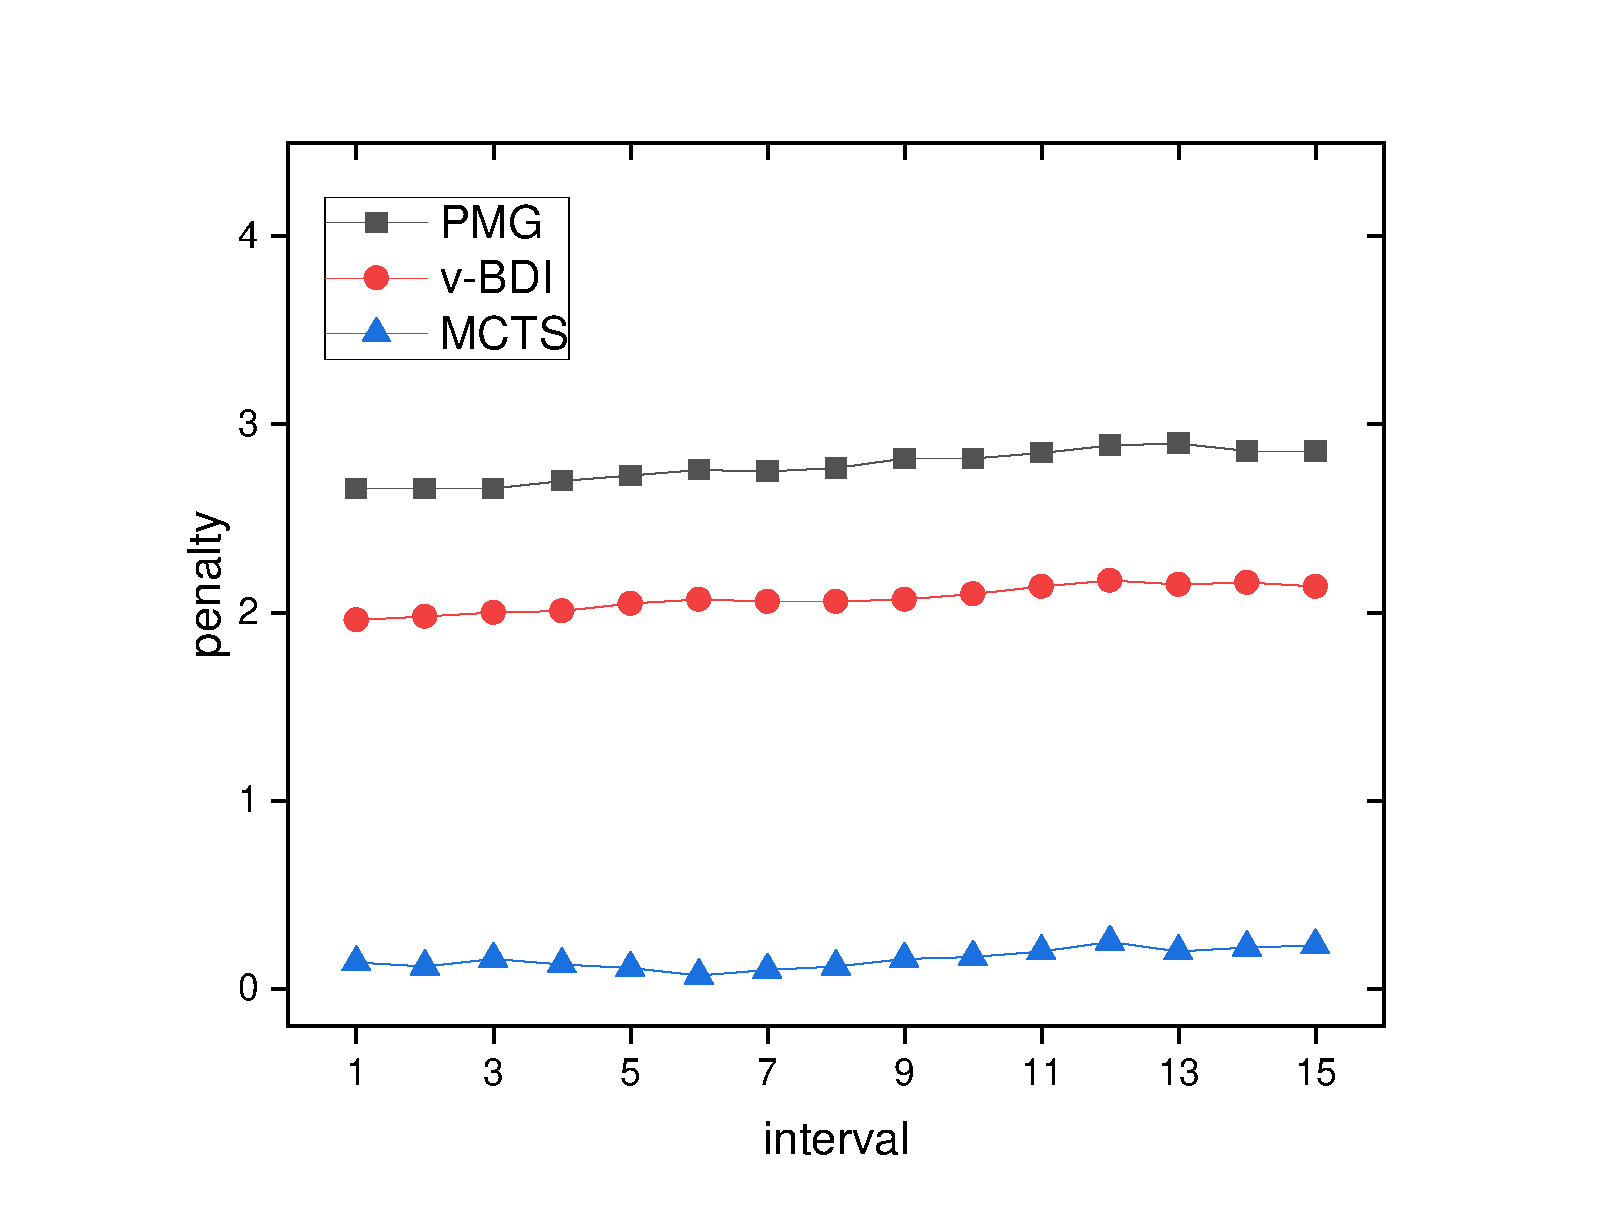
\includegraphics[scale=0.2]{inX_pY_fixCap60_complex}
  \caption{60容量}
  \captionsetup{justification=centering}
\end{subfigure}
\begin{subfigure}{.32\textwidth}
  \centering
  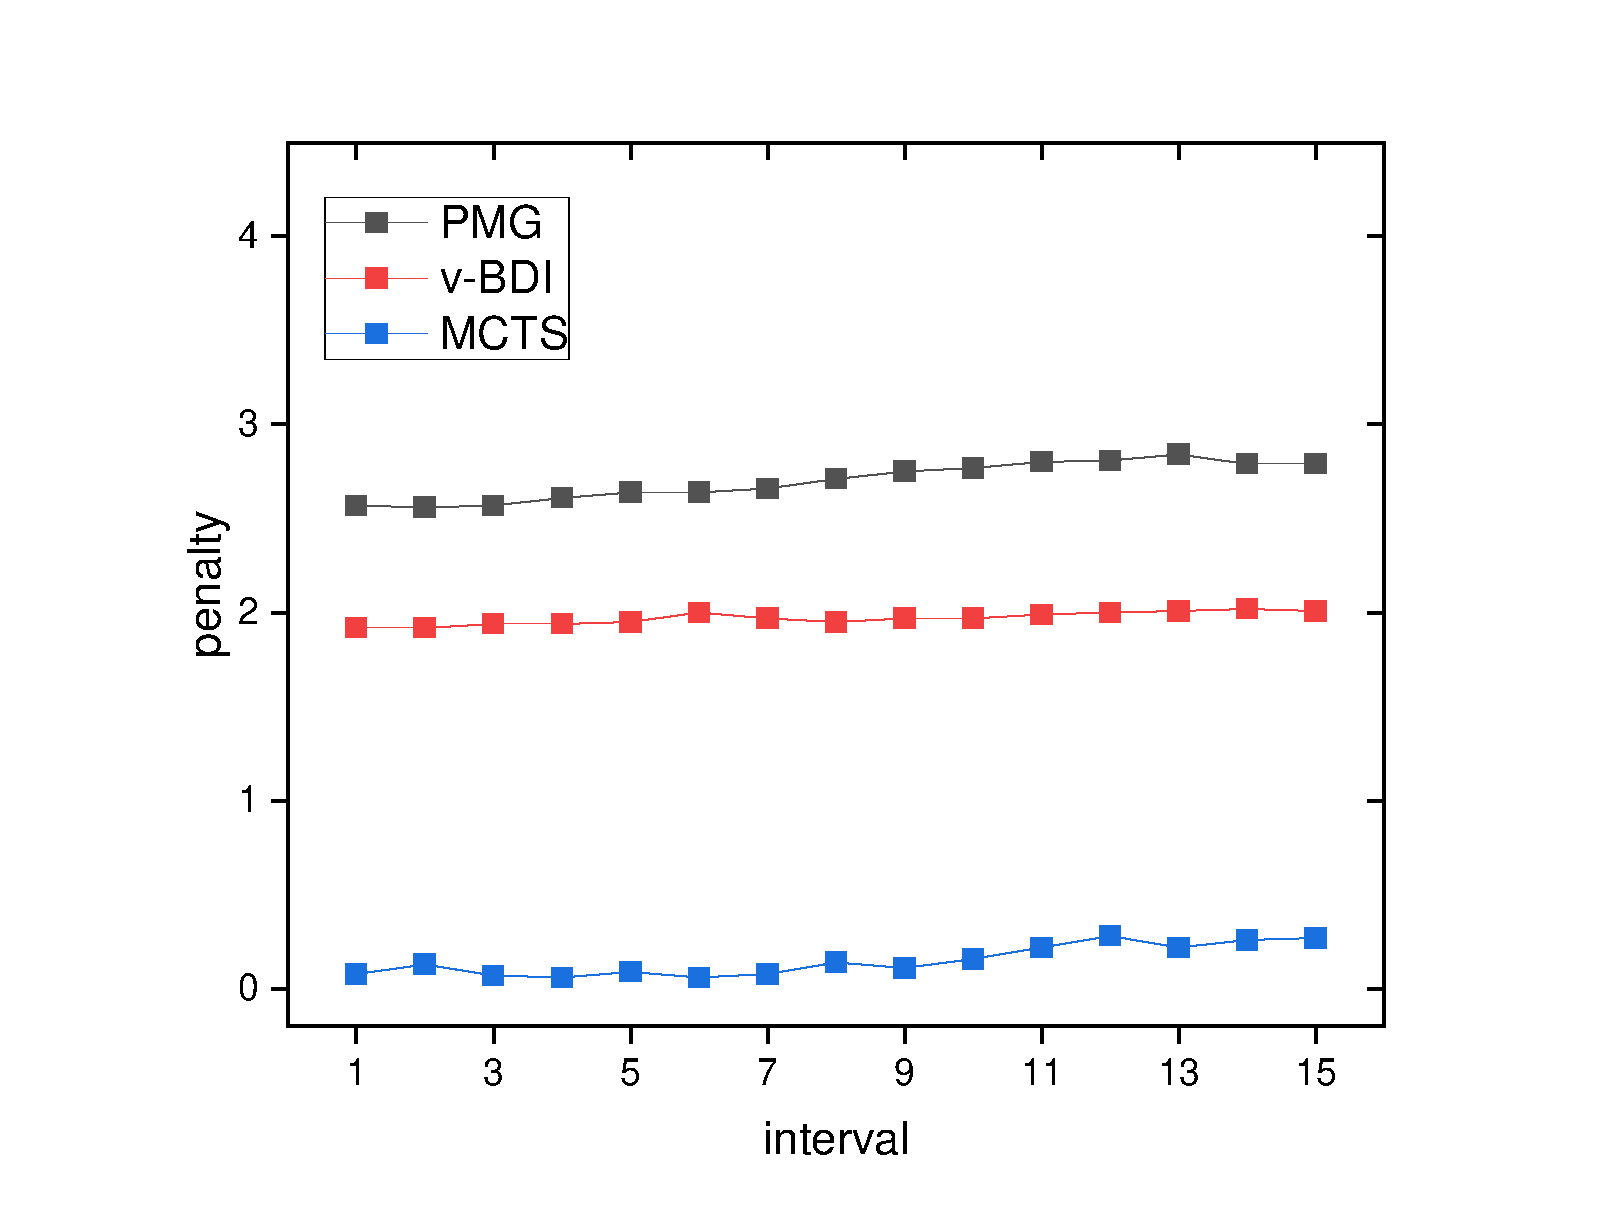
\includegraphics[scale=0.2]{inX_pY_fixCap140_complex}
  \caption{140容量}
  \captionsetup{justification=centering}
\end{subfigure}
\begin{subfigure}{.32\textwidth}
  \centering
  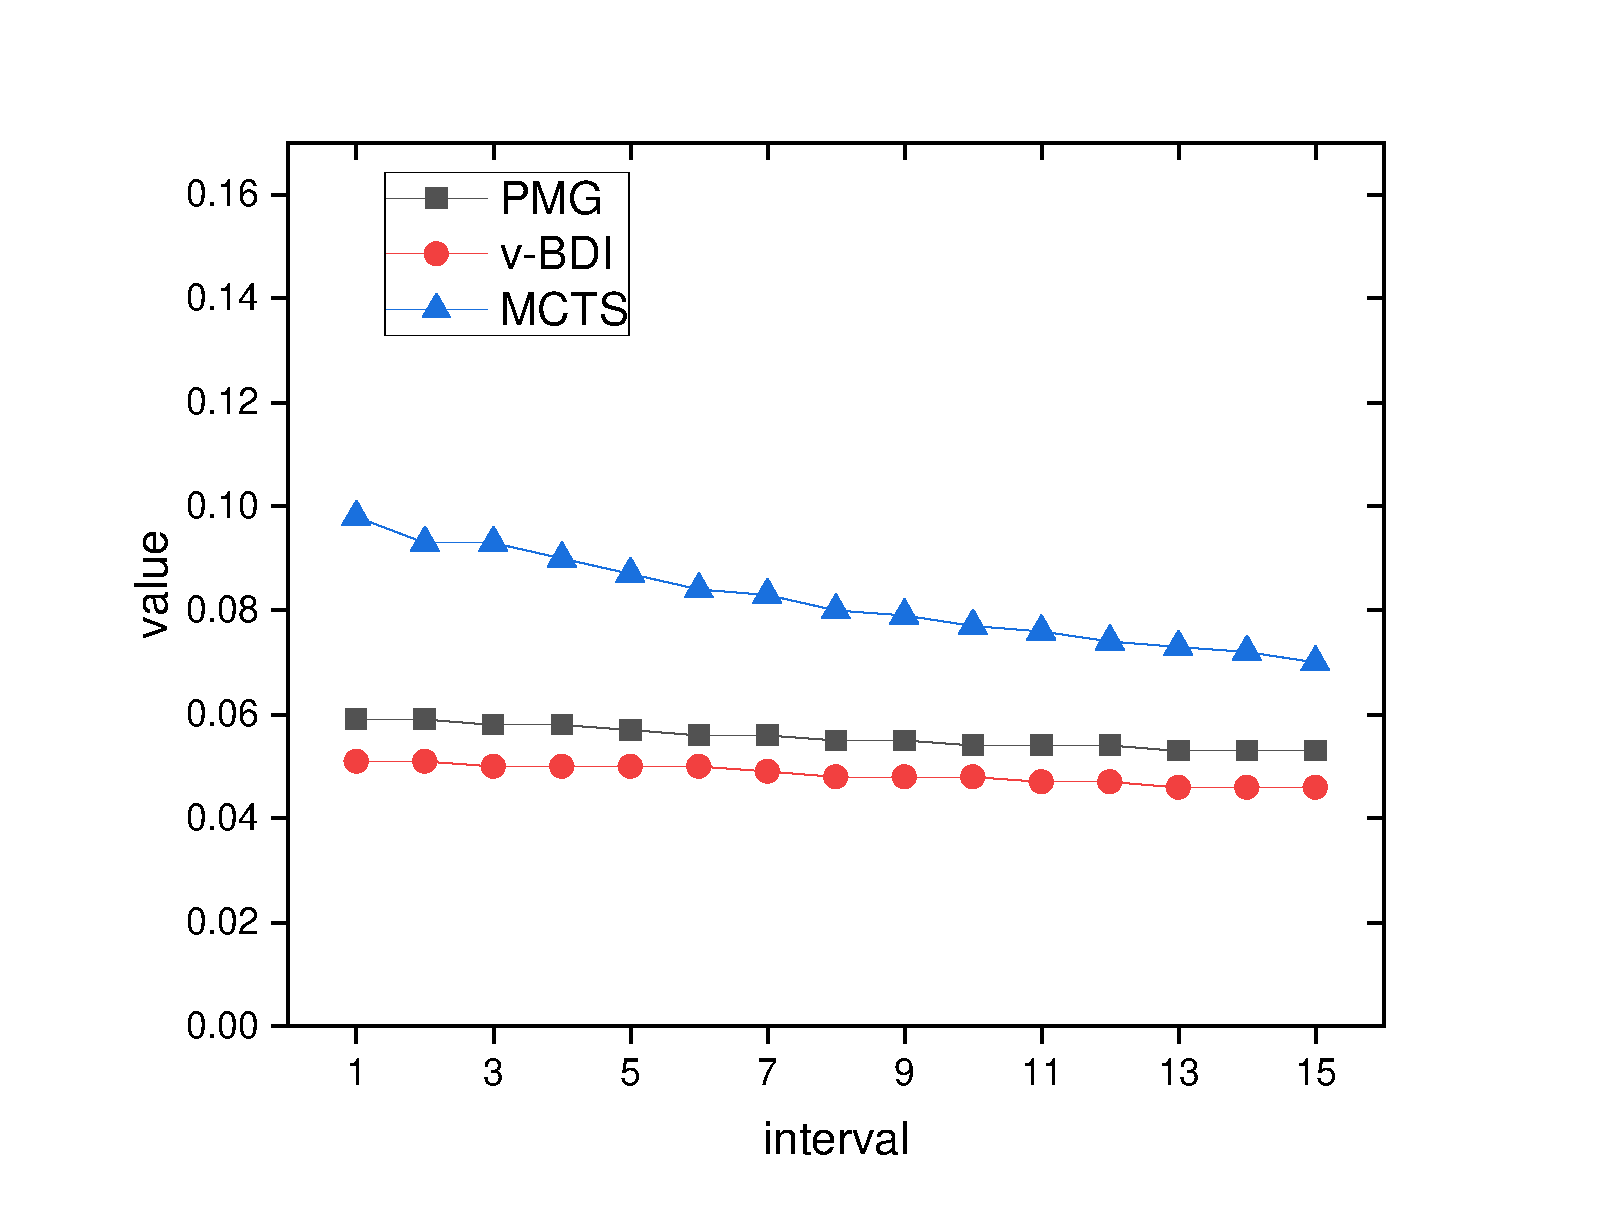
\includegraphics[scale=0.2]{inX_vY_fixCap40_complex}
  \caption{40容量}
  \captionsetup{justification=centering}
\end{subfigure}
\begin{subfigure}{.32\textwidth}
  \centering
  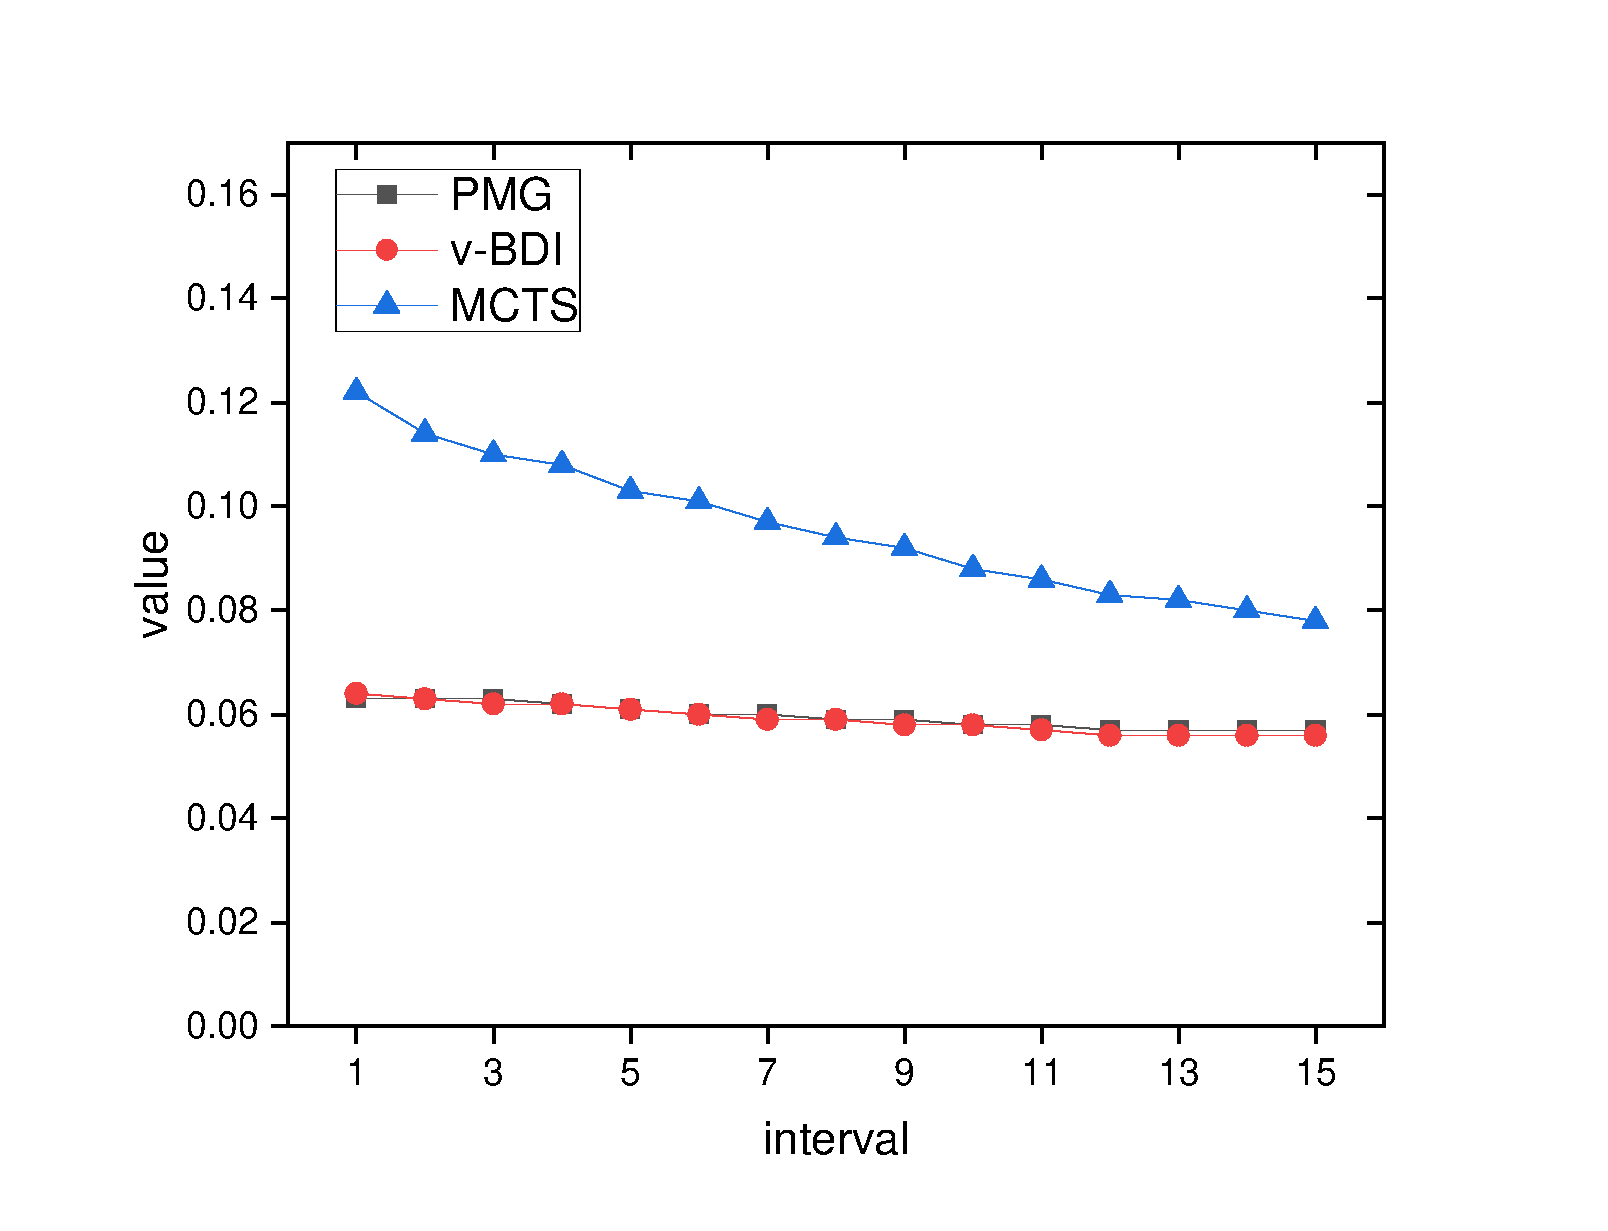
\includegraphics[scale=0.2]{inX_vY_fixCap60_complex}
  \caption{60容量}
  \captionsetup{justification=centering}
\end{subfigure}
\begin{subfigure}{.32\textwidth}
  \centering
  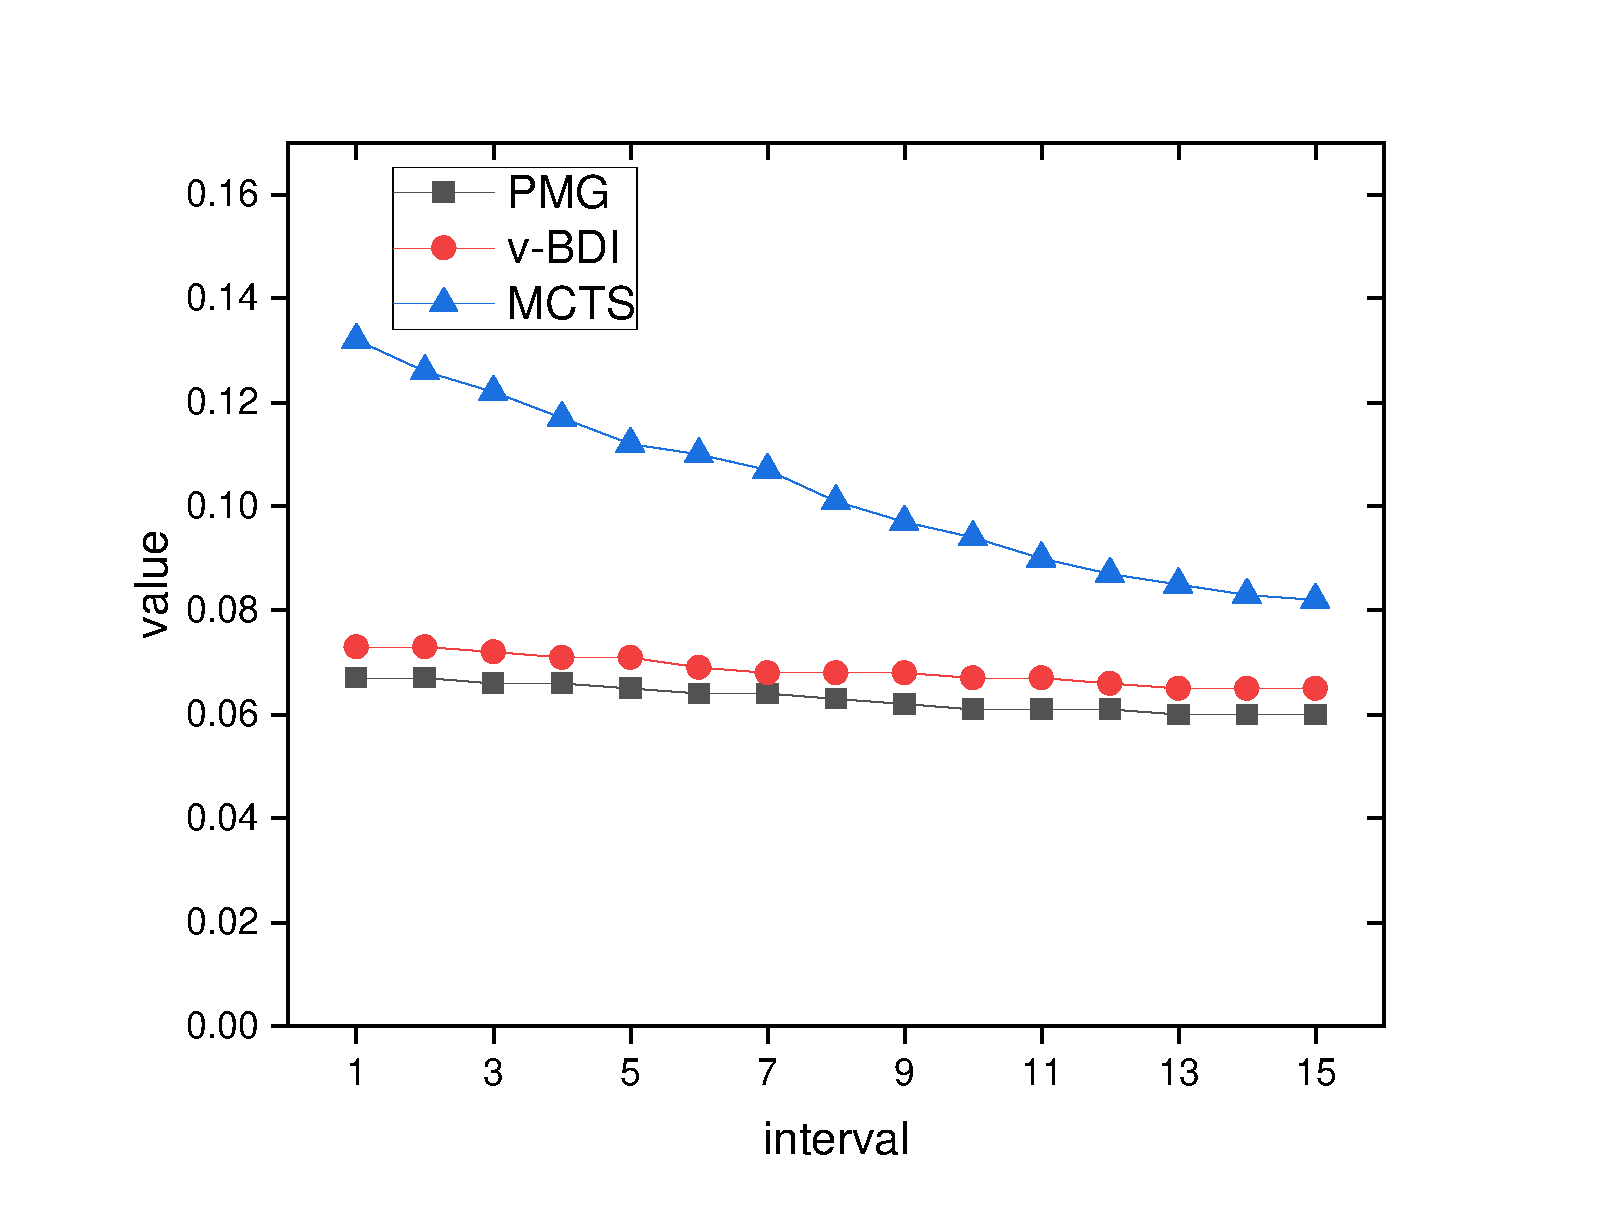
\includegraphics[scale=0.2]{inX_vY_fixCap140_complex}
  \caption{140容量}
  \captionsetup{justification=centering}
\end{subfigure}
\captionsetup{justification=centering}
\bicaption{复杂地形下的动态场景实验结果}{Experiment results in dynamic complex terrain scenario}
\label{fig:dynamic_complex}
\end{figure}


% \begin{figure*}[htb]
% \centering
% 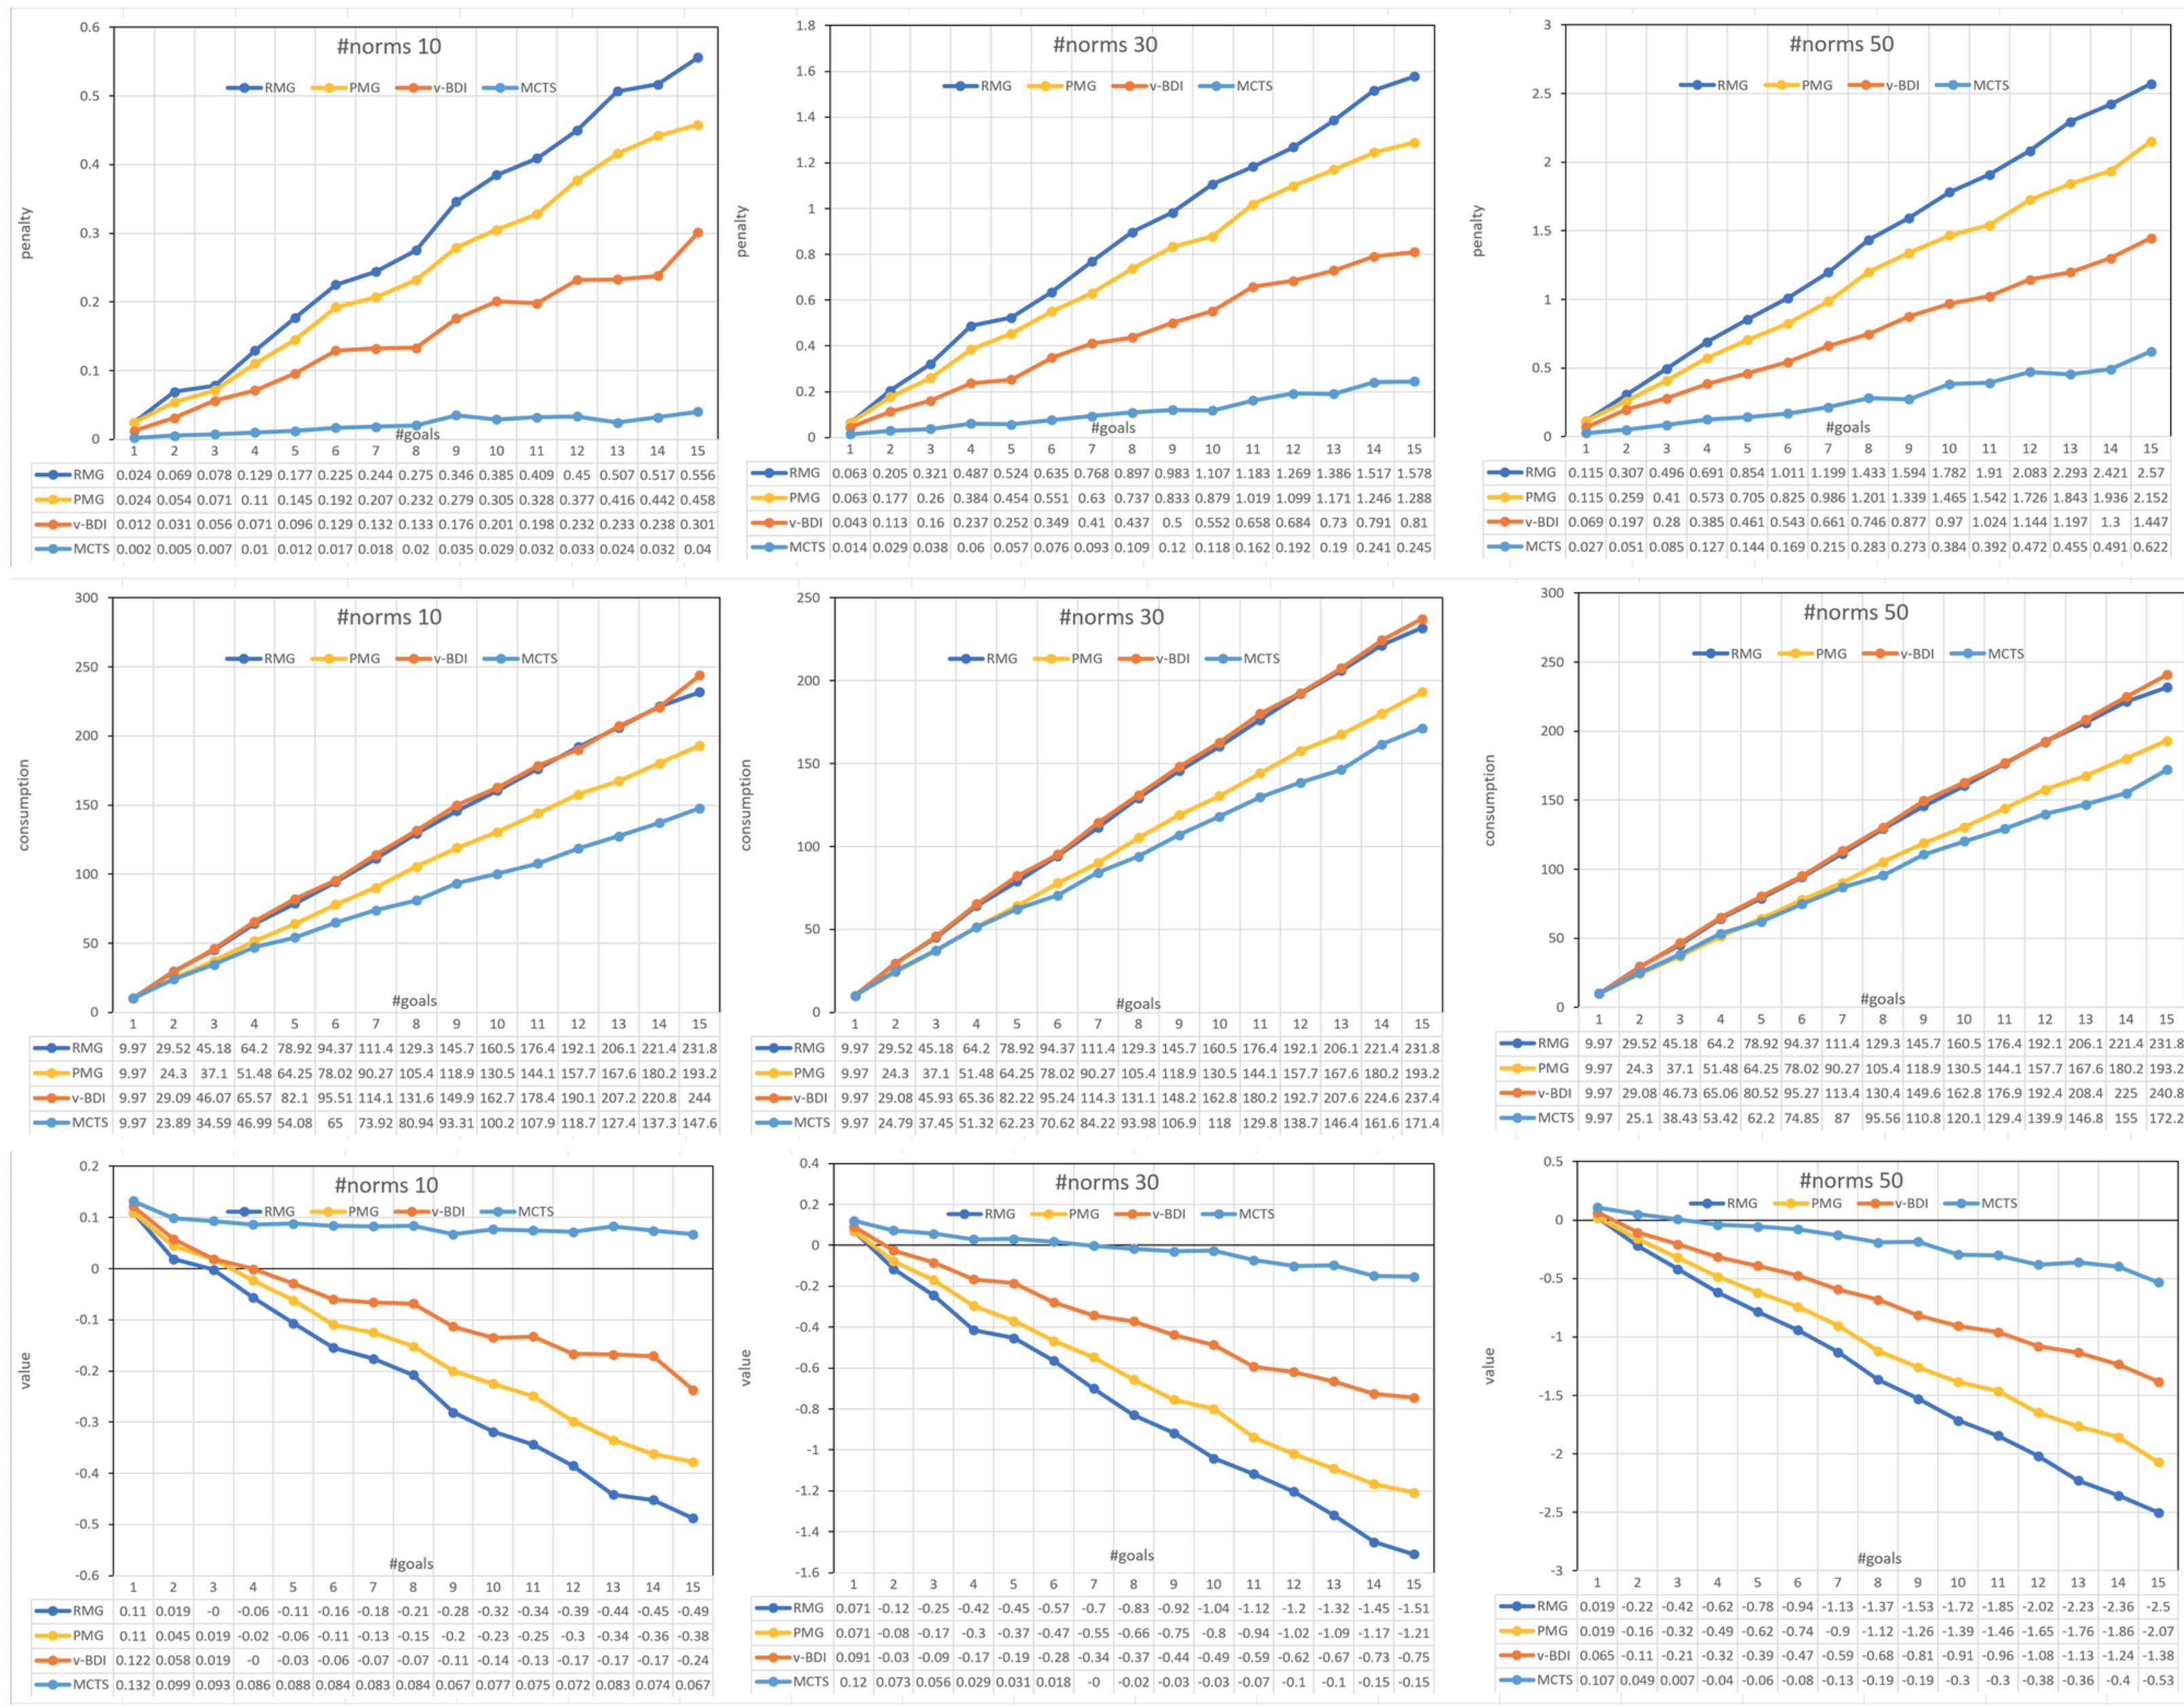
\includegraphics[width=0.9\textwidth]{./figs/ltl_low_battery}
% \bicaption{低电池容量下的实验结果}{experimental results in low battery}
% \label{fig:ltl_low}
% \end{figure*}


\subsection{简单地形实验}
在简单的地形场景中,地图被中间的一个长斜坡分为两部分:左侧和右侧。左侧部分包括x坐标小于10的单元格;右侧部分包括x坐标大于或等于10的单元格。以下假设左边是高地,右边是低地。当智能体从右到左(即从低地到高地)时会违反norm并受到相应的惩罚。确切的地形设置如图\ref{fig:simple}所示。
\begin{figure}[H]
\centering
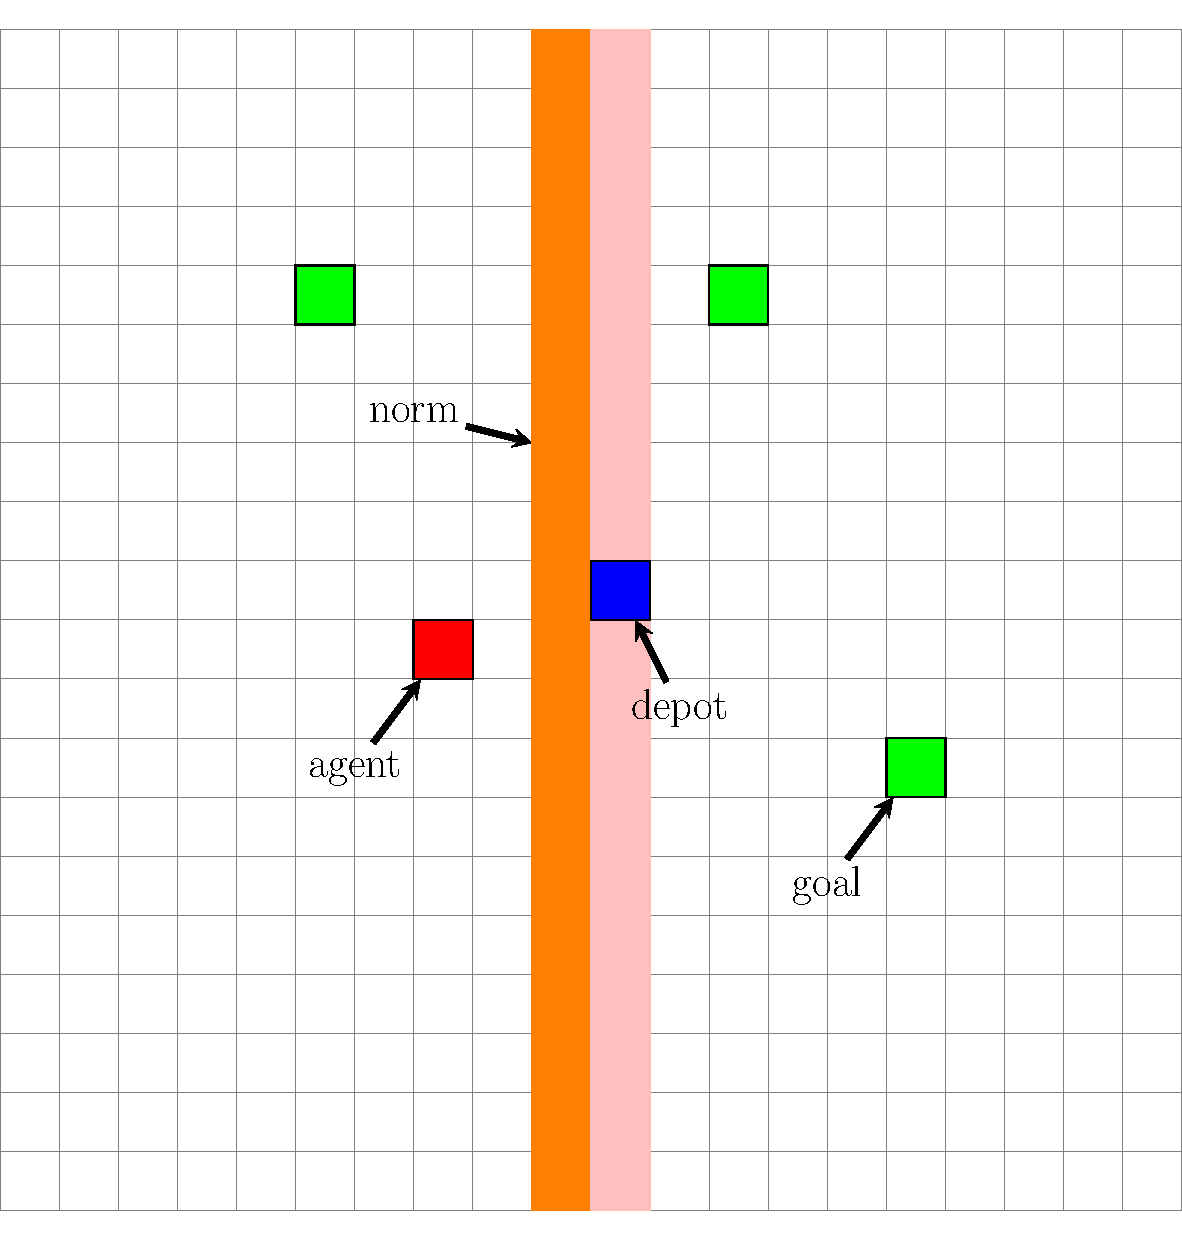
\includegraphics[scale=0.5]{MR_simple_norm_example.pdf}
\captionsetup{justification=centering}
\bicaption{简单地形场景}{Simple terrain scenario}
\label{fig:simple}
\end{figure}

\paragraph{静态场景}
和复杂地形在静态场景下的设定类似,本实验考虑了智能体在静态环境中的执行的情景,在该场景中,所有目标在初始时给定。在不同的容量设置中,将要实现的目标数量从1个改变到15个不等。具体实验结果如图\ref{fig:static_simple}所示。


从图中可以看出,油耗结果与复杂地形场景相似。
惩罚值方面,在该简单地形环境设置中,即使容量很大,与PMG相比,v-BDI也没有优势。因为不存在v-BDI可以避免违反规范而PMG不能的情况。
总体效用结果也符合预期。随着容量变大,PMG和v-BDI之间的差异变小。与复杂的地形环境相比,MCTS的性能提升更为明显,因为智能体先在一边实现目标,然后在另一边目标情况下,MCTS能更方便地利用协同效应。
\begin{figure}[H]
\centering
\begin{subfigure}{.32\textwidth}
  \centering
  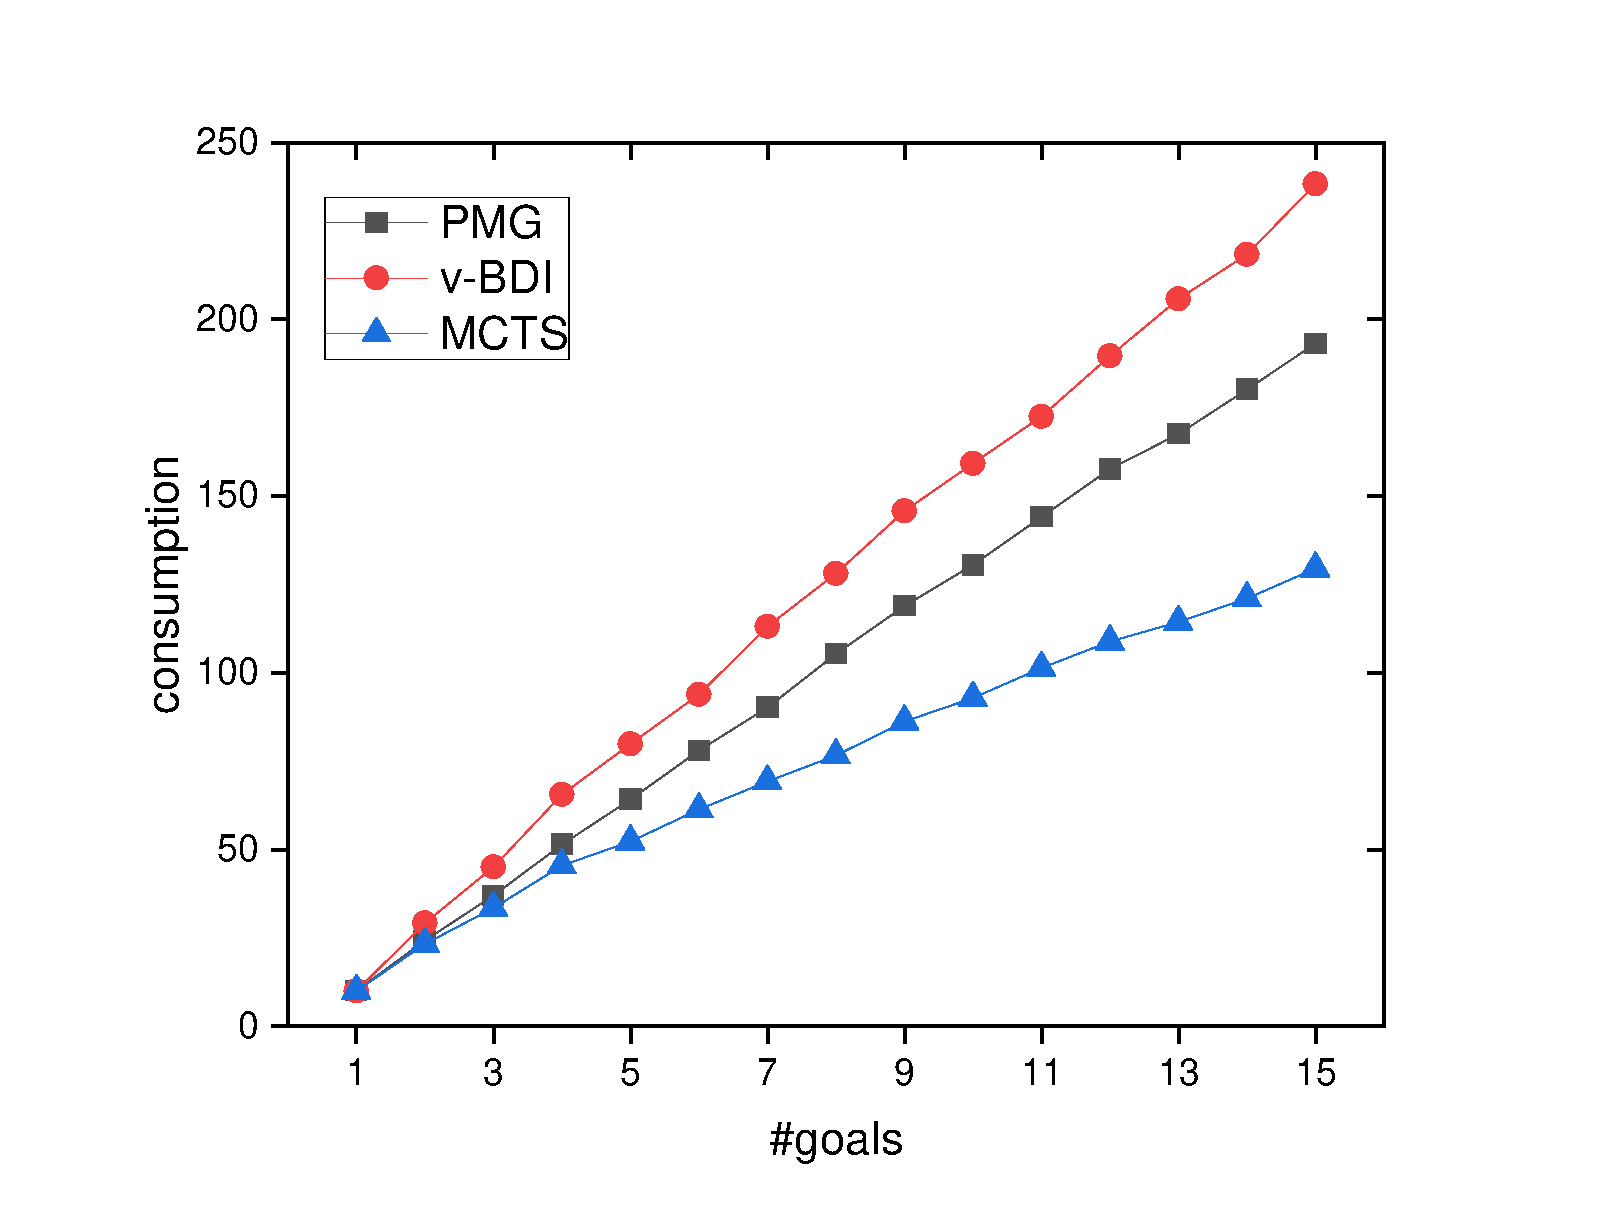
\includegraphics[scale=0.2]{gX_consY_fixCap40_simple}
  \caption{40容量}
  \captionsetup{justification=centering}
\end{subfigure}
\begin{subfigure}{.32\textwidth}
  \centering
  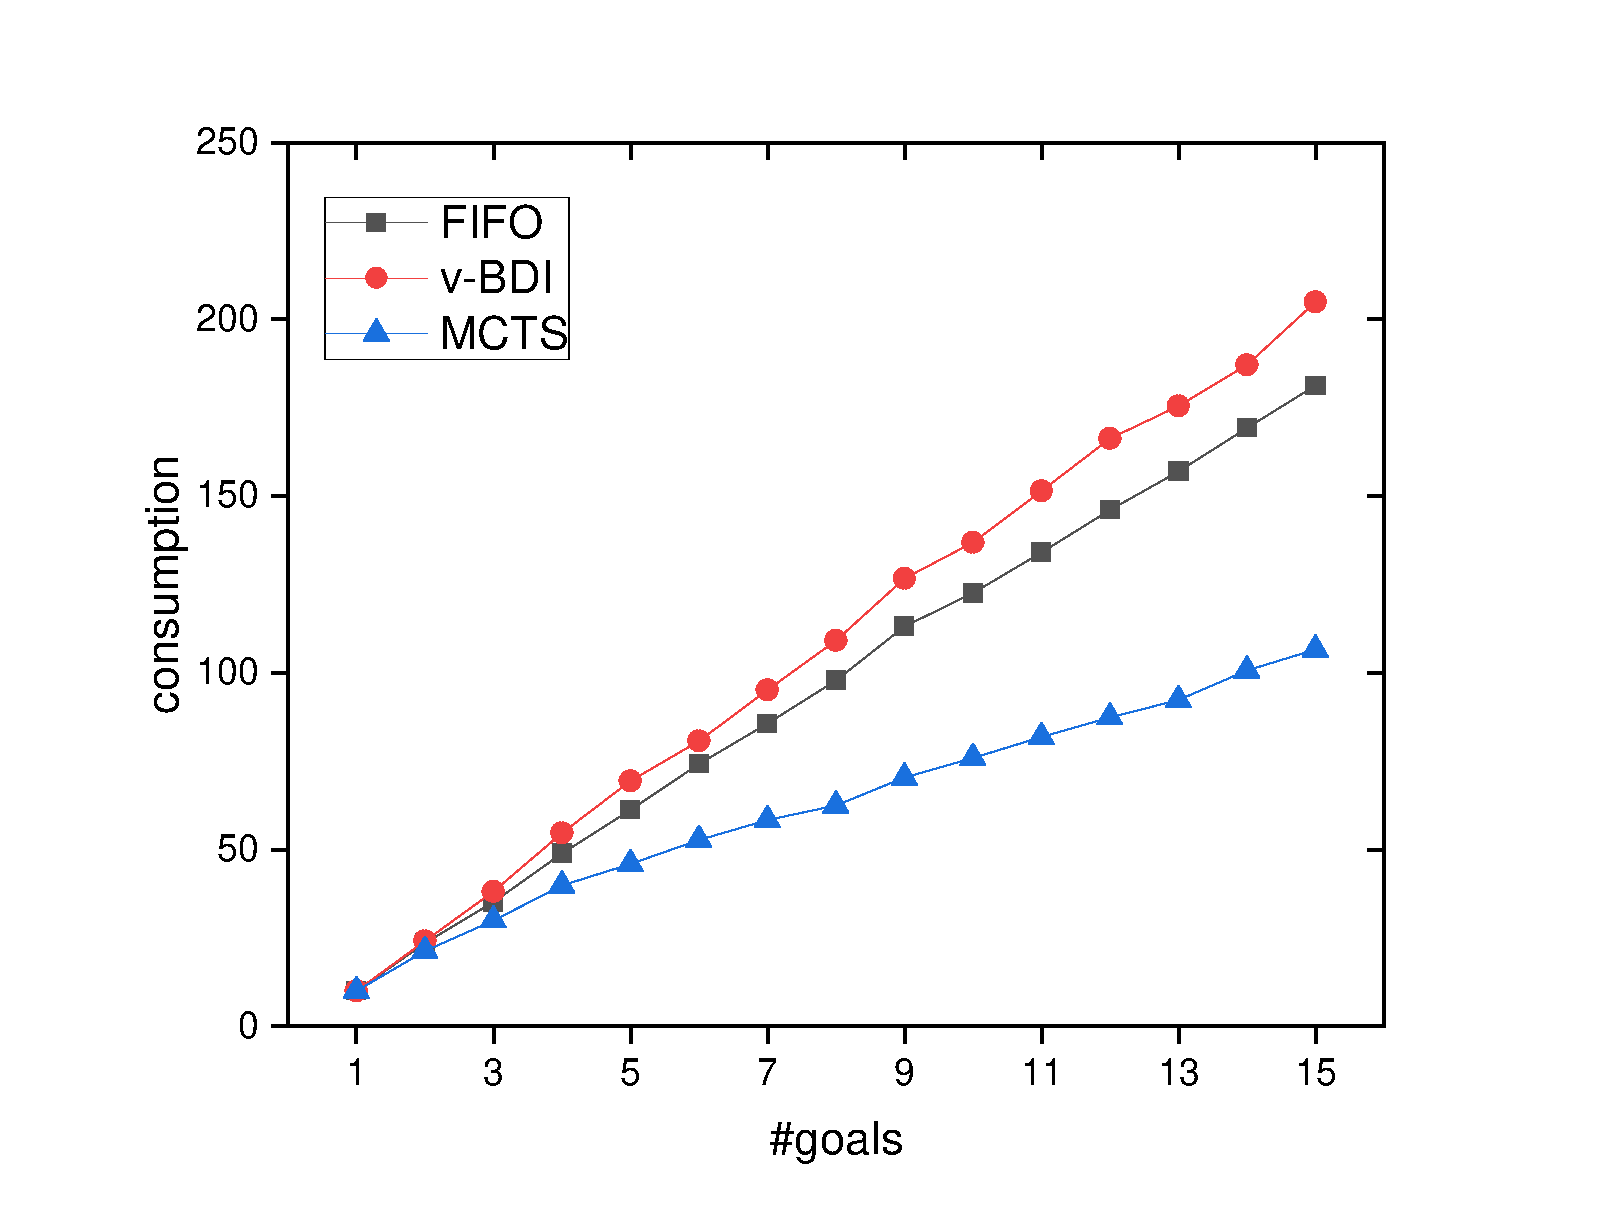
\includegraphics[scale=0.2]{gX_consY_fixCap60_simple}
  \caption{60容量}
  \captionsetup{justification=centering}
\end{subfigure}
\begin{subfigure}{.32\textwidth}
  \centering
  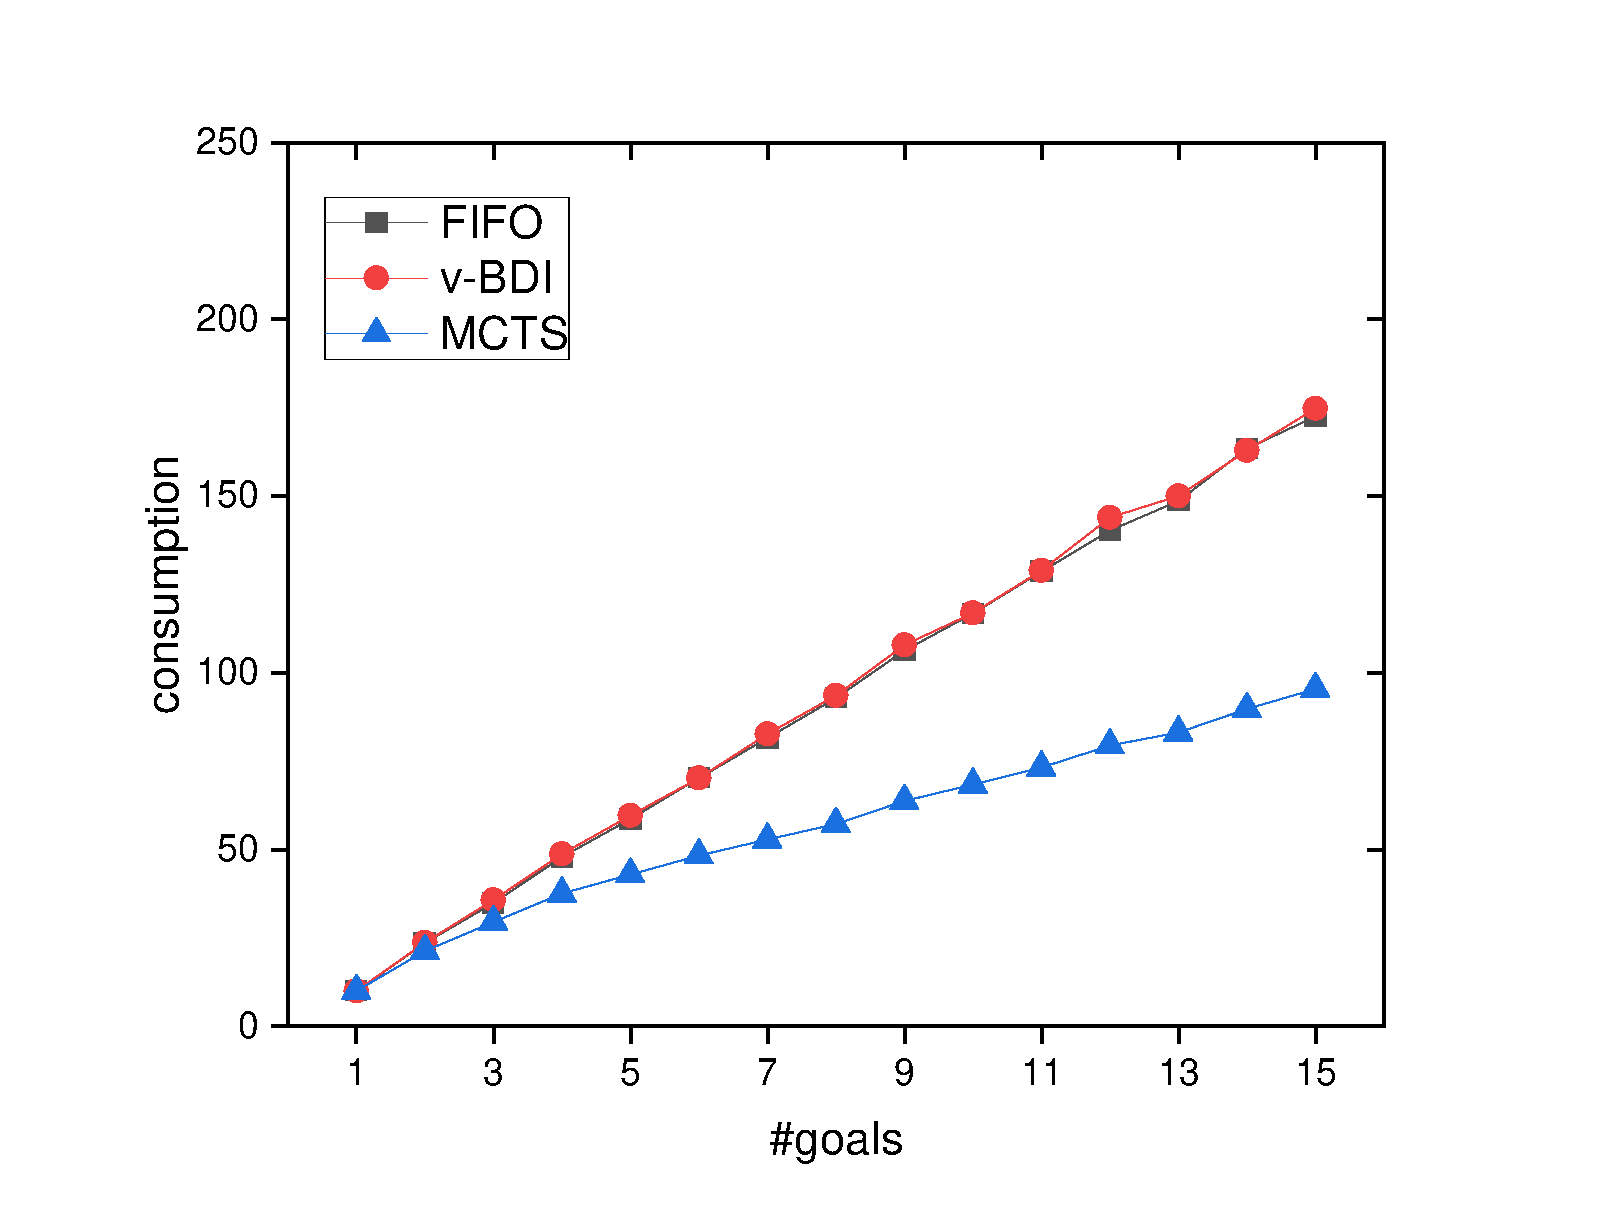
\includegraphics[scale=0.2]{gX_consY_fixCap140_simple}
  \caption{140容量}
  \captionsetup{justification=centering}
\end{subfigure}
\begin{subfigure}{.32\textwidth}
  \centering
  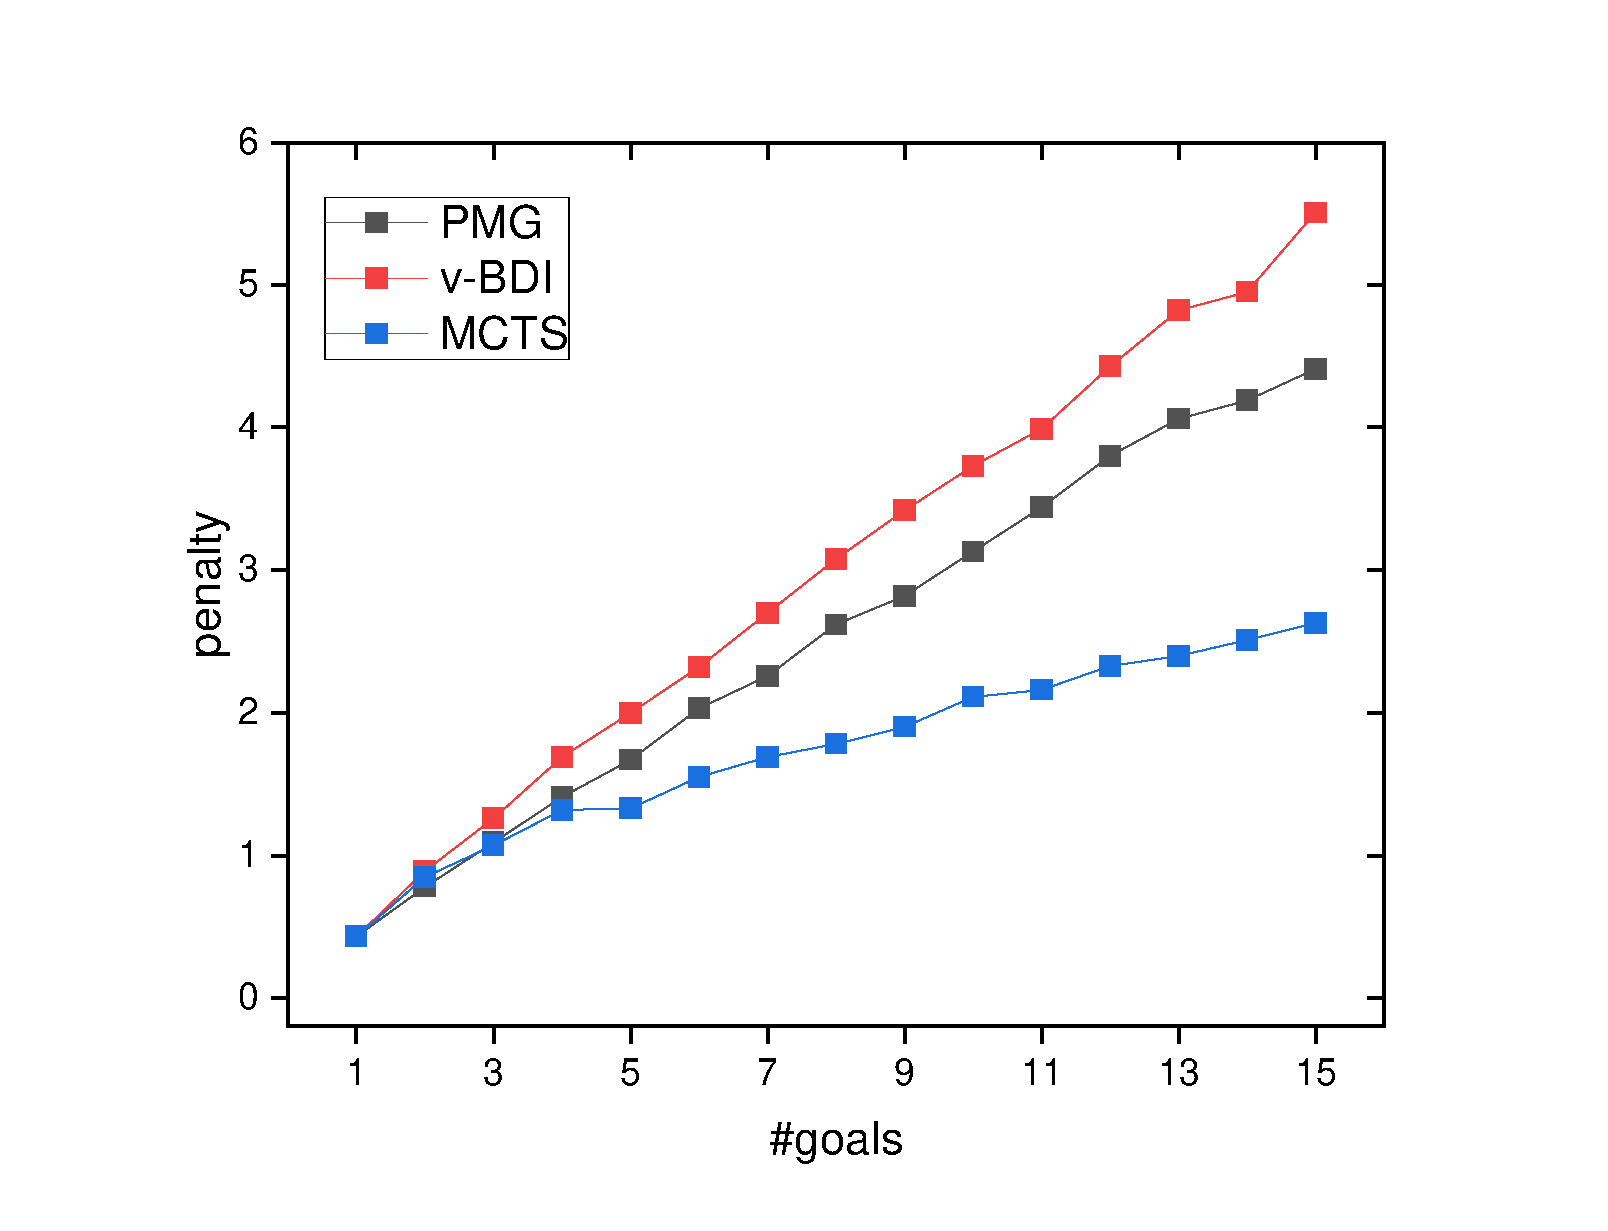
\includegraphics[scale=0.2]{gX_pY_fixCap40_simple}
  \caption{40容量}
  \captionsetup{justification=centering}
\end{subfigure}
\begin{subfigure}{.32\textwidth}
  \centering
  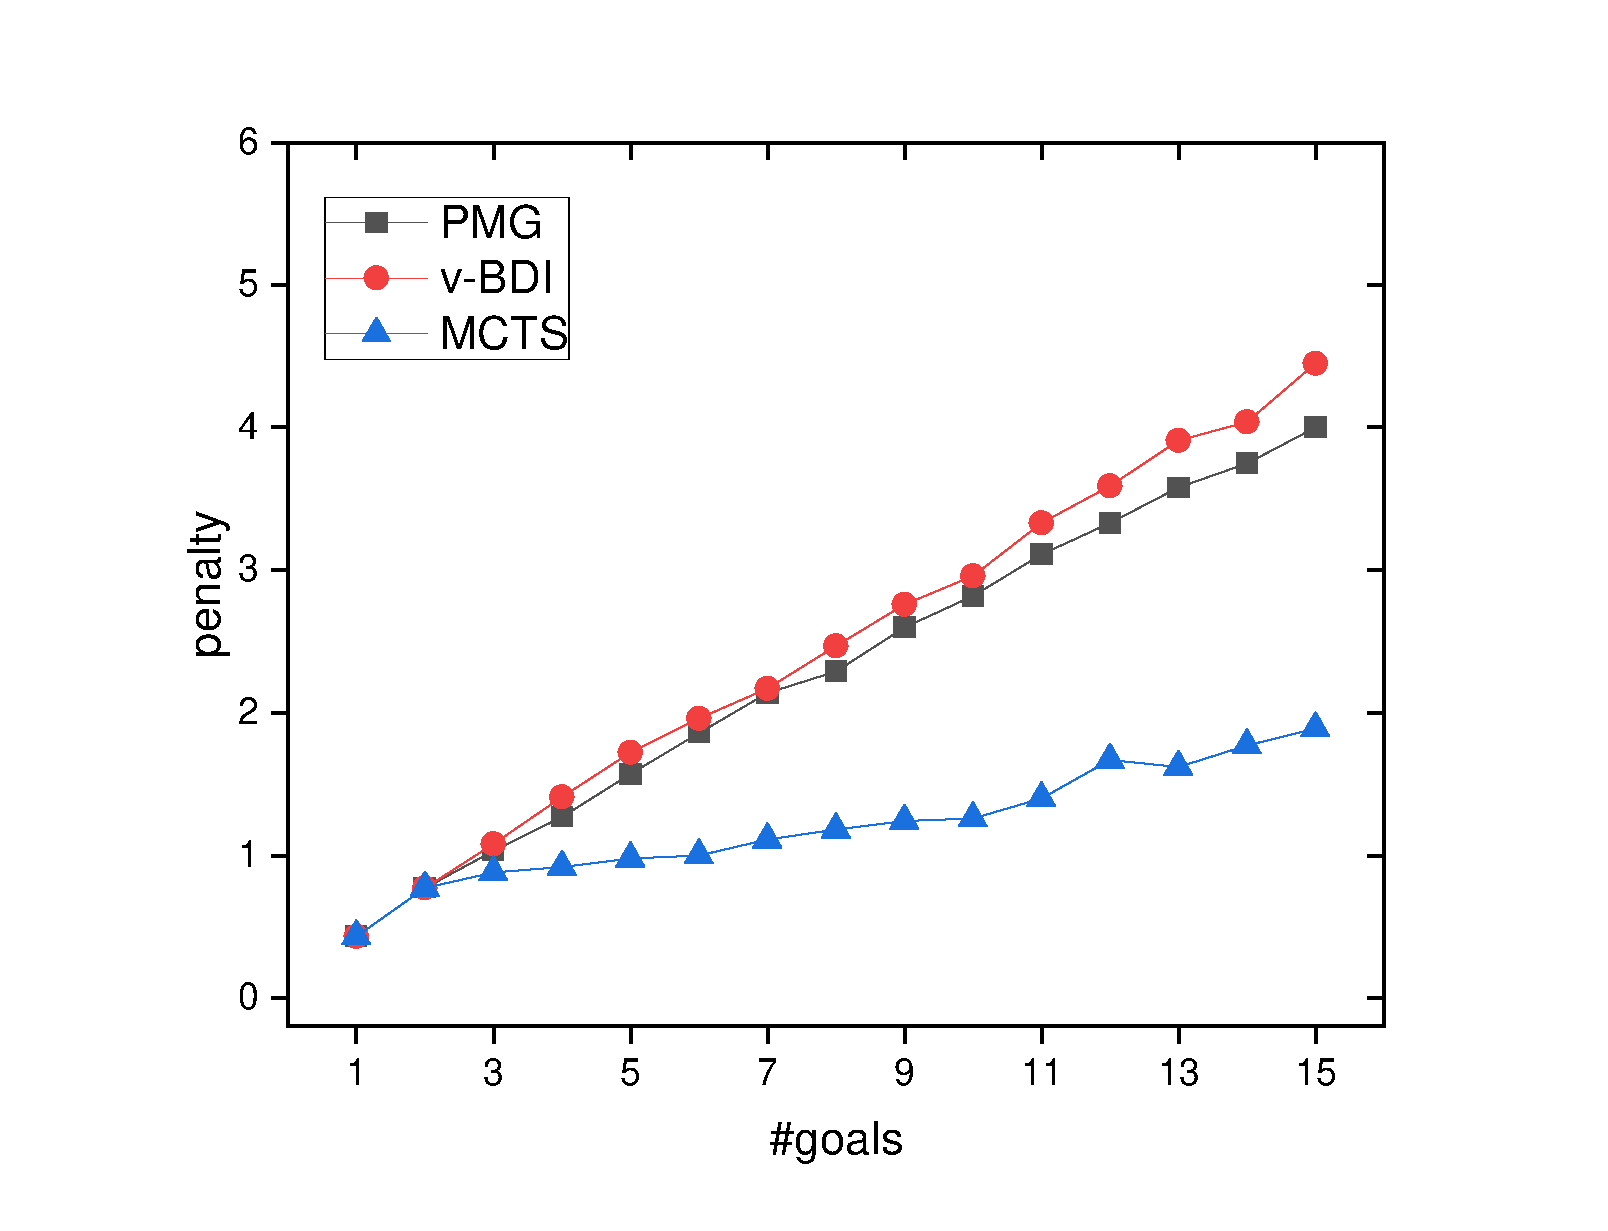
\includegraphics[scale=0.2]{gX_pY_fixCap60_simple}
  \caption{60容量}
  \captionsetup{justification=centering}
\end{subfigure}
\begin{subfigure}{.32\textwidth}
  \centering
  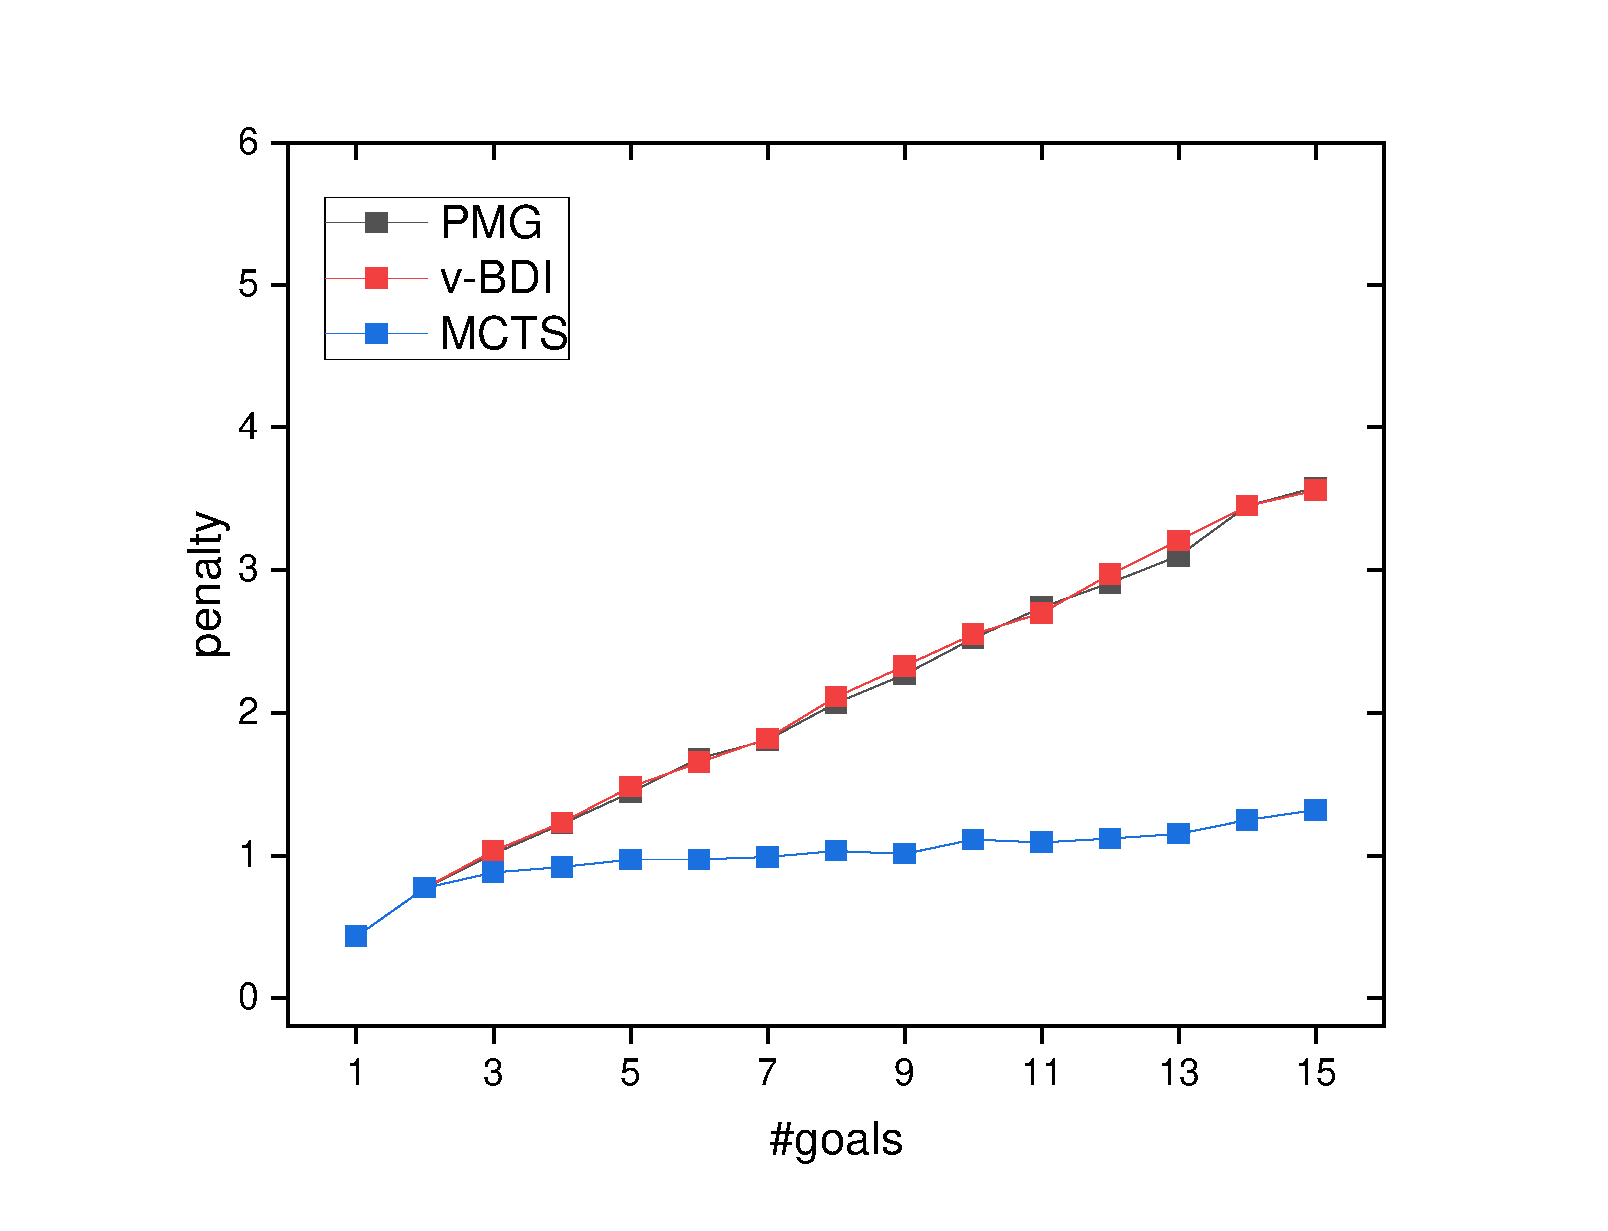
\includegraphics[scale=0.2]{gX_pY_fixCap140_simple}
  \caption{140容量}
  \captionsetup{justification=centering}
\end{subfigure}
\begin{subfigure}{.32\textwidth}
  \centering
  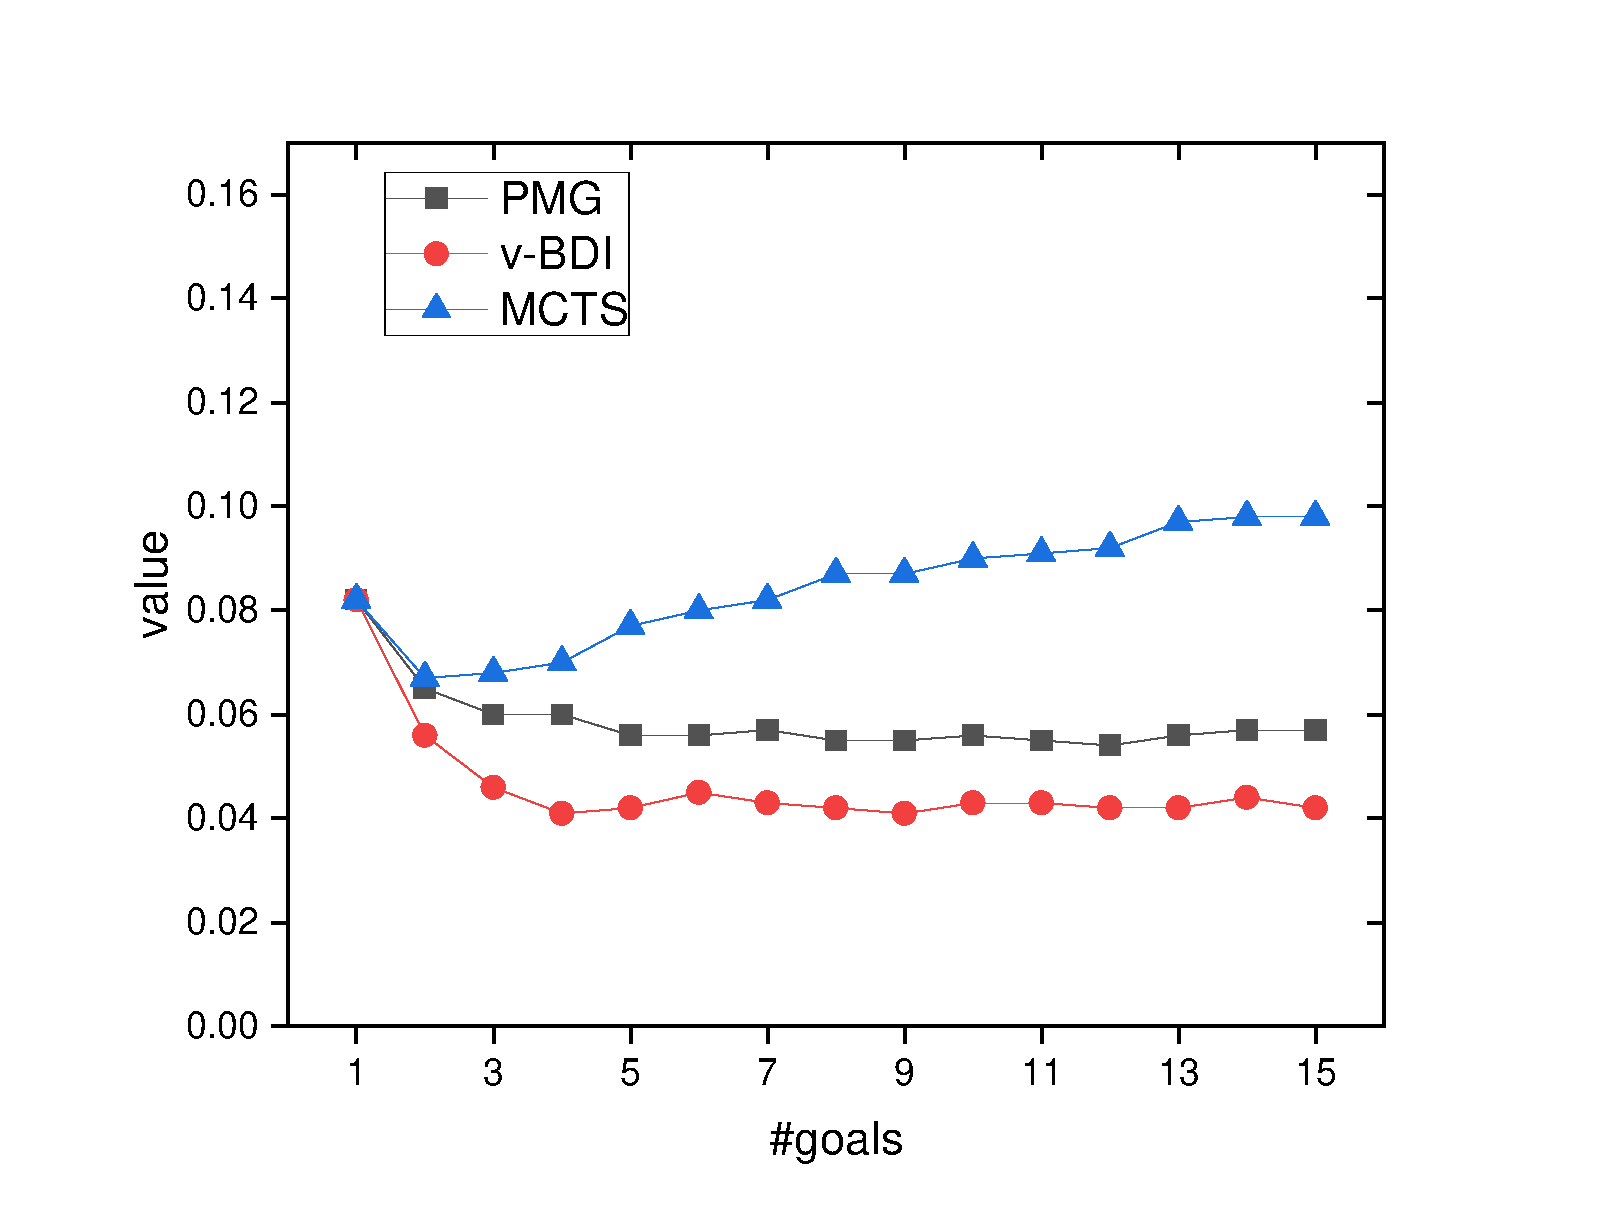
\includegraphics[scale=0.2]{gX_vY_fixCap40_simple}
  \caption{40容量}
  \captionsetup{justification=centering}
\end{subfigure}
\begin{subfigure}{.32\textwidth}
  \centering
  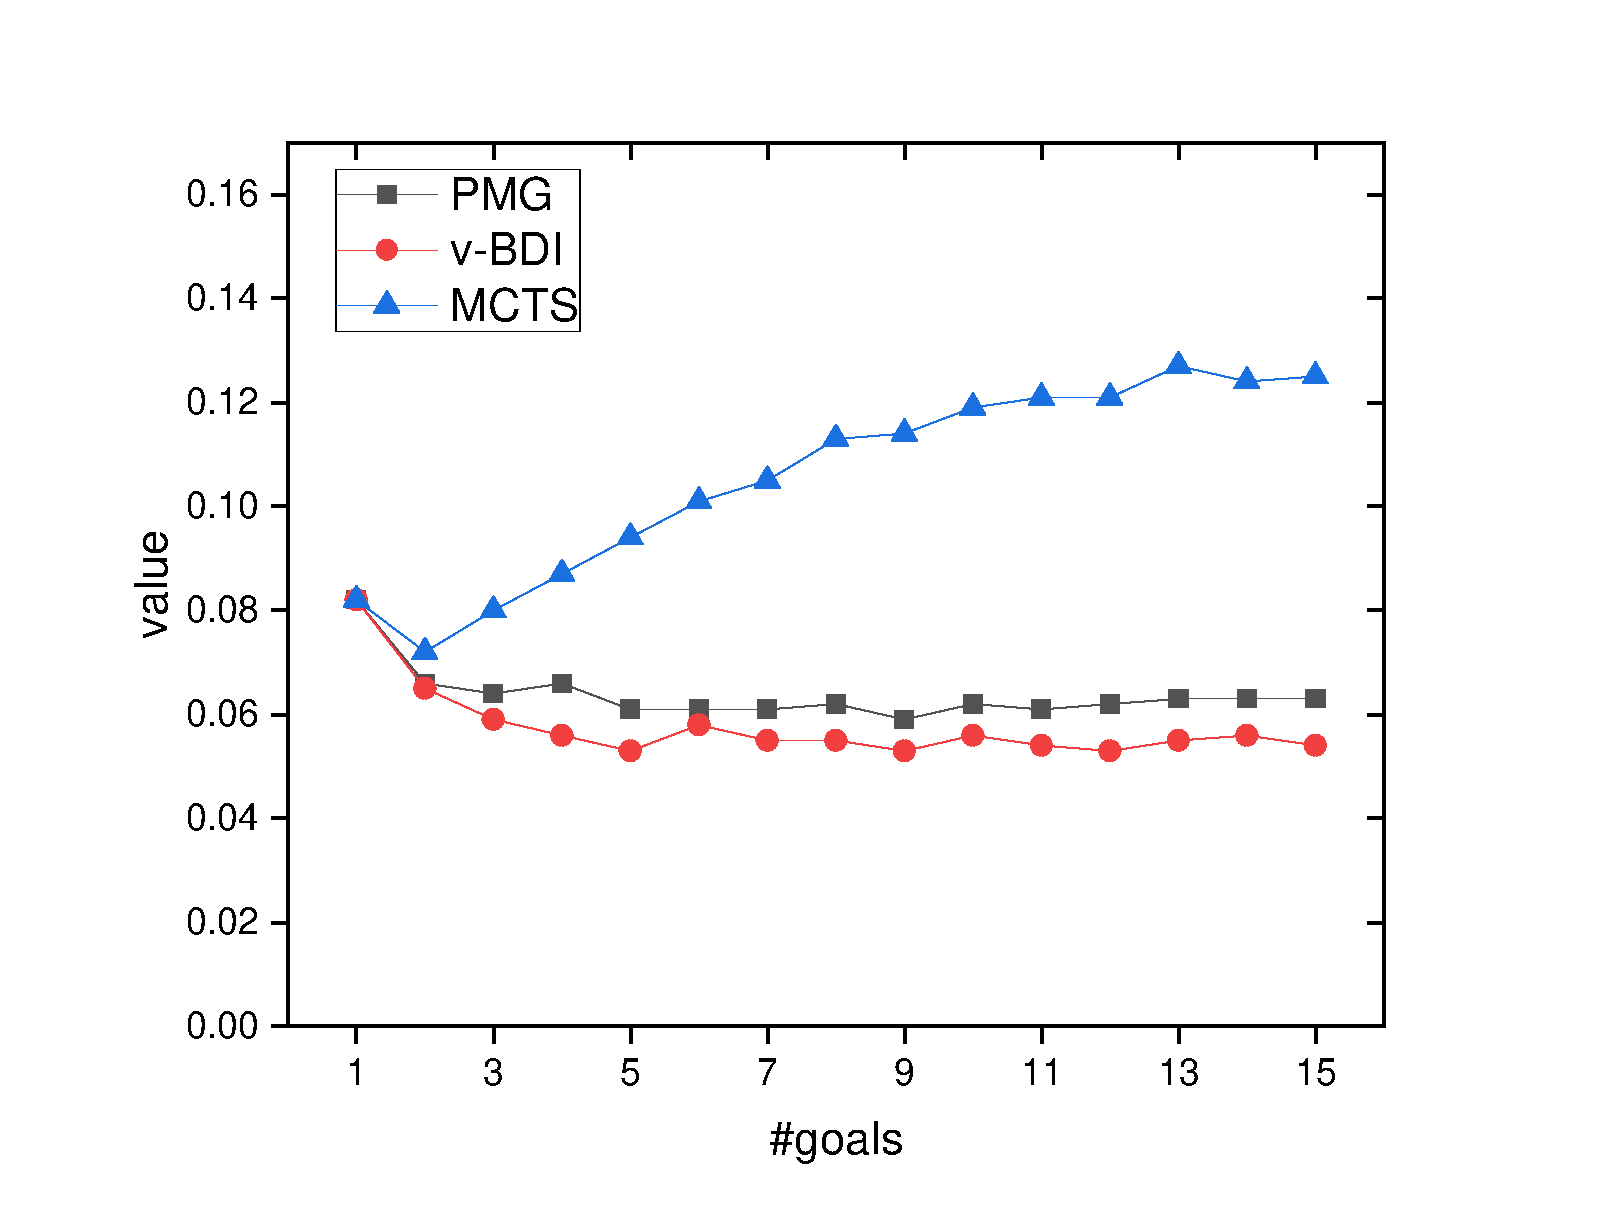
\includegraphics[scale=0.2]{gX_vY_fixCap60_simple}
  \caption{60容量}
  \captionsetup{justification=centering}
\end{subfigure}
\begin{subfigure}{.32\textwidth}
  \centering
  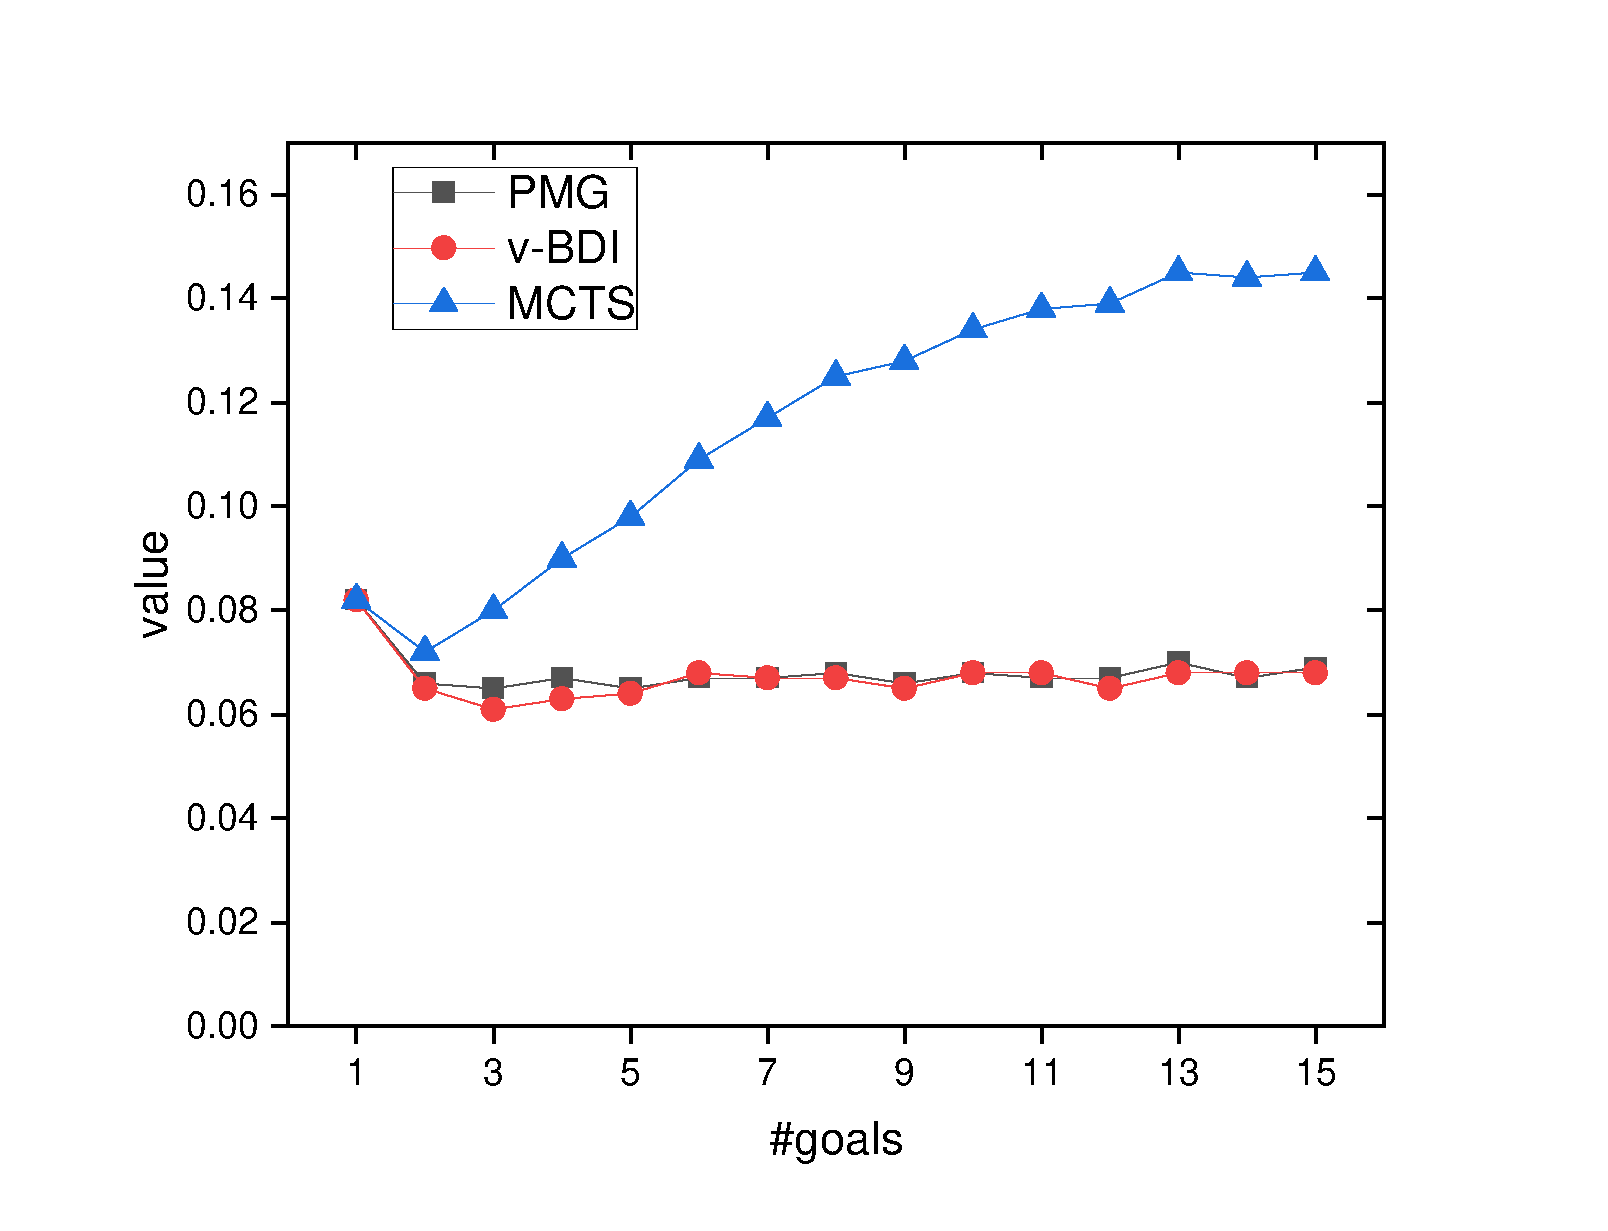
\includegraphics[scale=0.2]{gX_vY_fixCap140_simple}
  \caption{140容量}
  \captionsetup{justification=centering}
\end{subfigure}
\captionsetup{justification=centering}
\bicaption{简单地形下的静态场景实验结果}{Experiment results in static simple terrain scenario}
\label{fig:static_simple}
\end{figure}

\paragraph{动态场景}
以下的实验假设最初给出两个目标(如果顶层目标的总数为1,那么在场景开始时只发布一个目标),其余目标每$n$步分配一次。具体实验结果如图\ref{fig:dynamic_simple}所示。

\begin{figure}[H]
\centering
\begin{subfigure}{.32\textwidth}
  \centering
  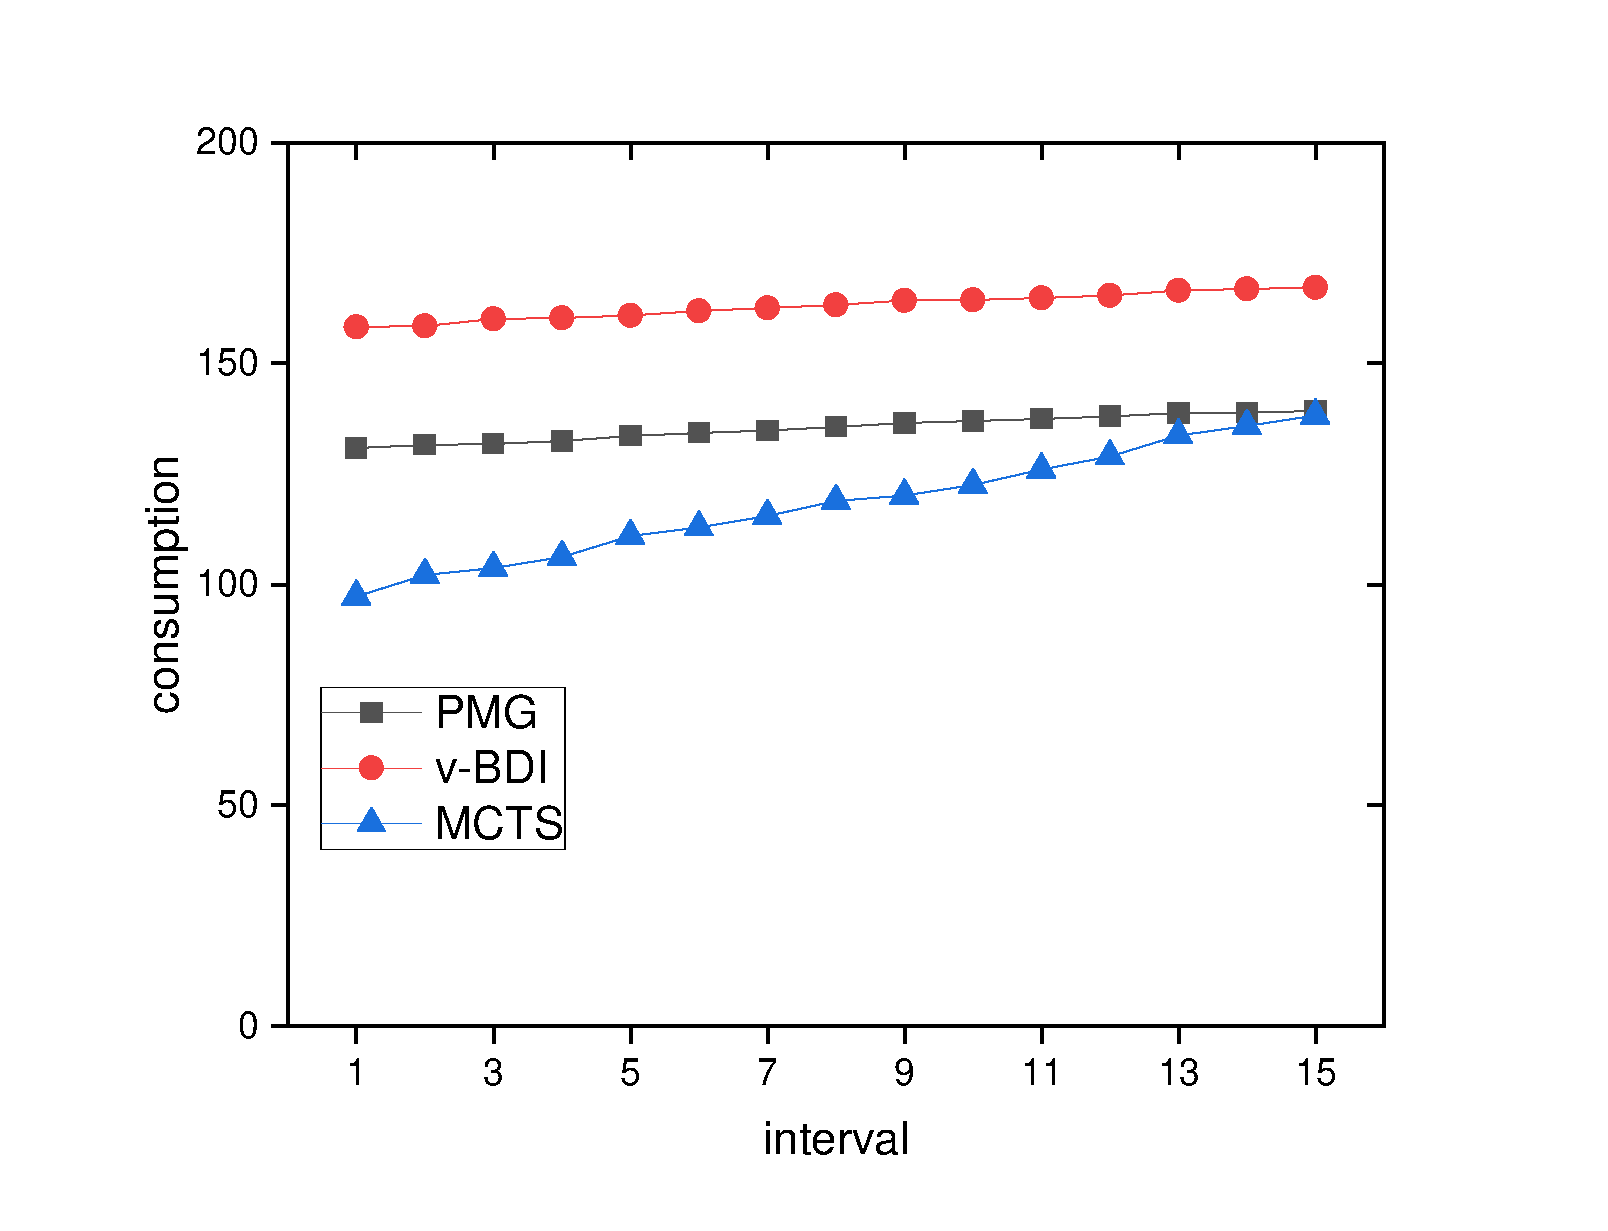
\includegraphics[scale=0.2]{inX_consY_fixCap40_simple}
  \caption{40容量}
  \captionsetup{justification=centering}
\end{subfigure}
\begin{subfigure}{.32\textwidth}
  \centering
  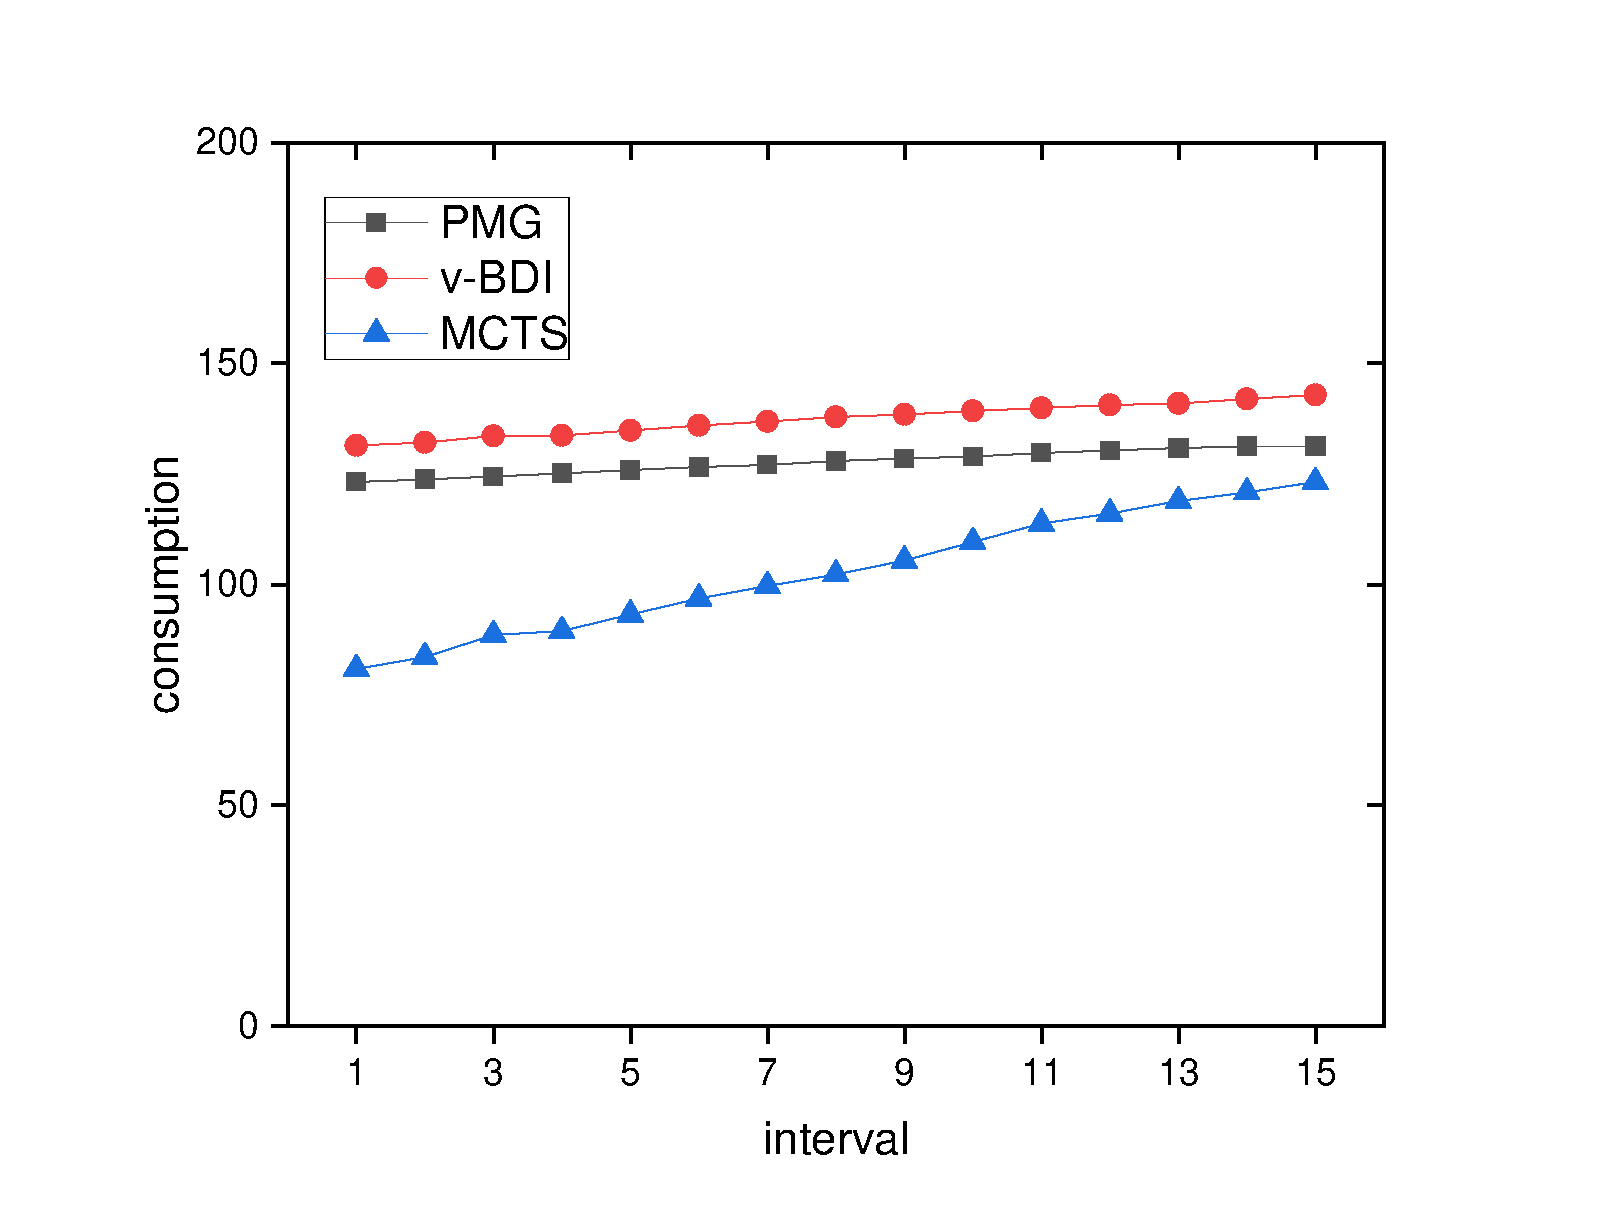
\includegraphics[scale=0.2]{inX_consY_fixCap60_simple}
  \caption{60容量}
  \captionsetup{justification=centering}
\end{subfigure}
\begin{subfigure}{.32\textwidth}
  \centering
  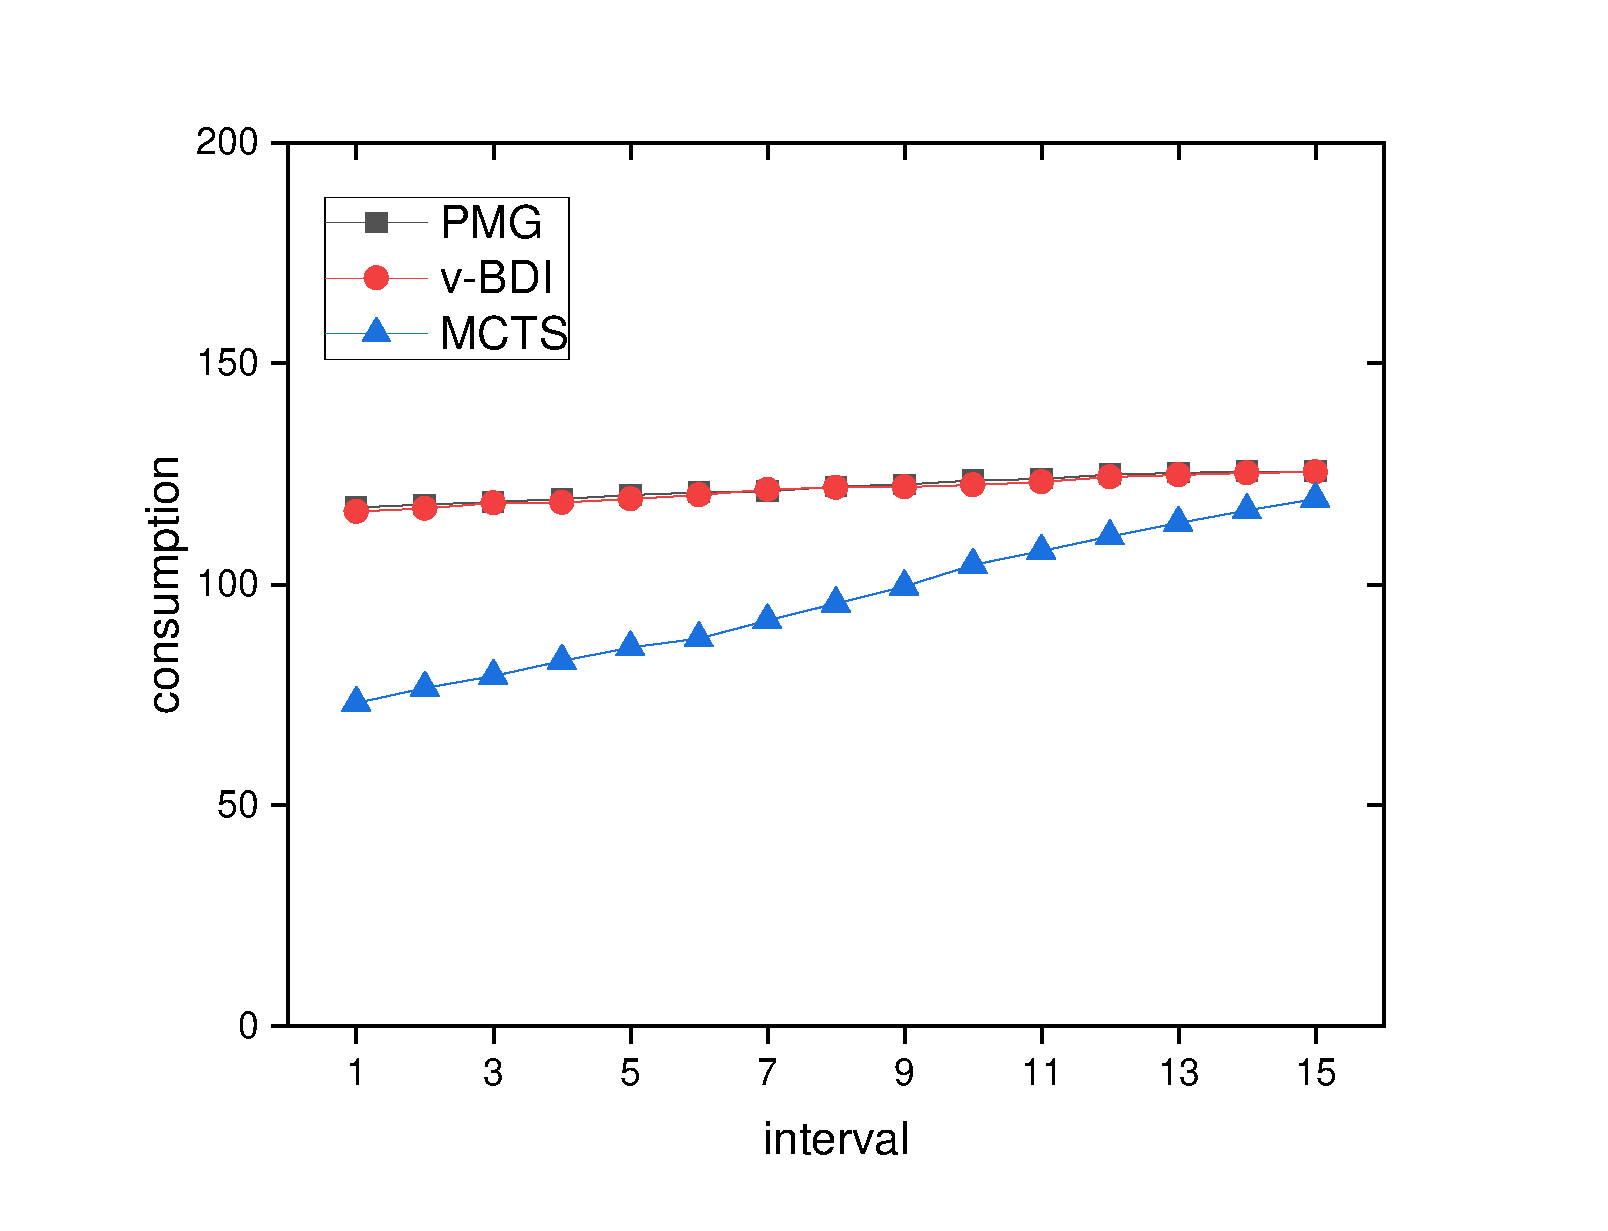
\includegraphics[scale=0.2]{inX_consY_fixCap140_simple}
  \caption{140容量}
  \captionsetup{justification=centering}
\end{subfigure}
\begin{subfigure}{.32\textwidth}
  \centering
  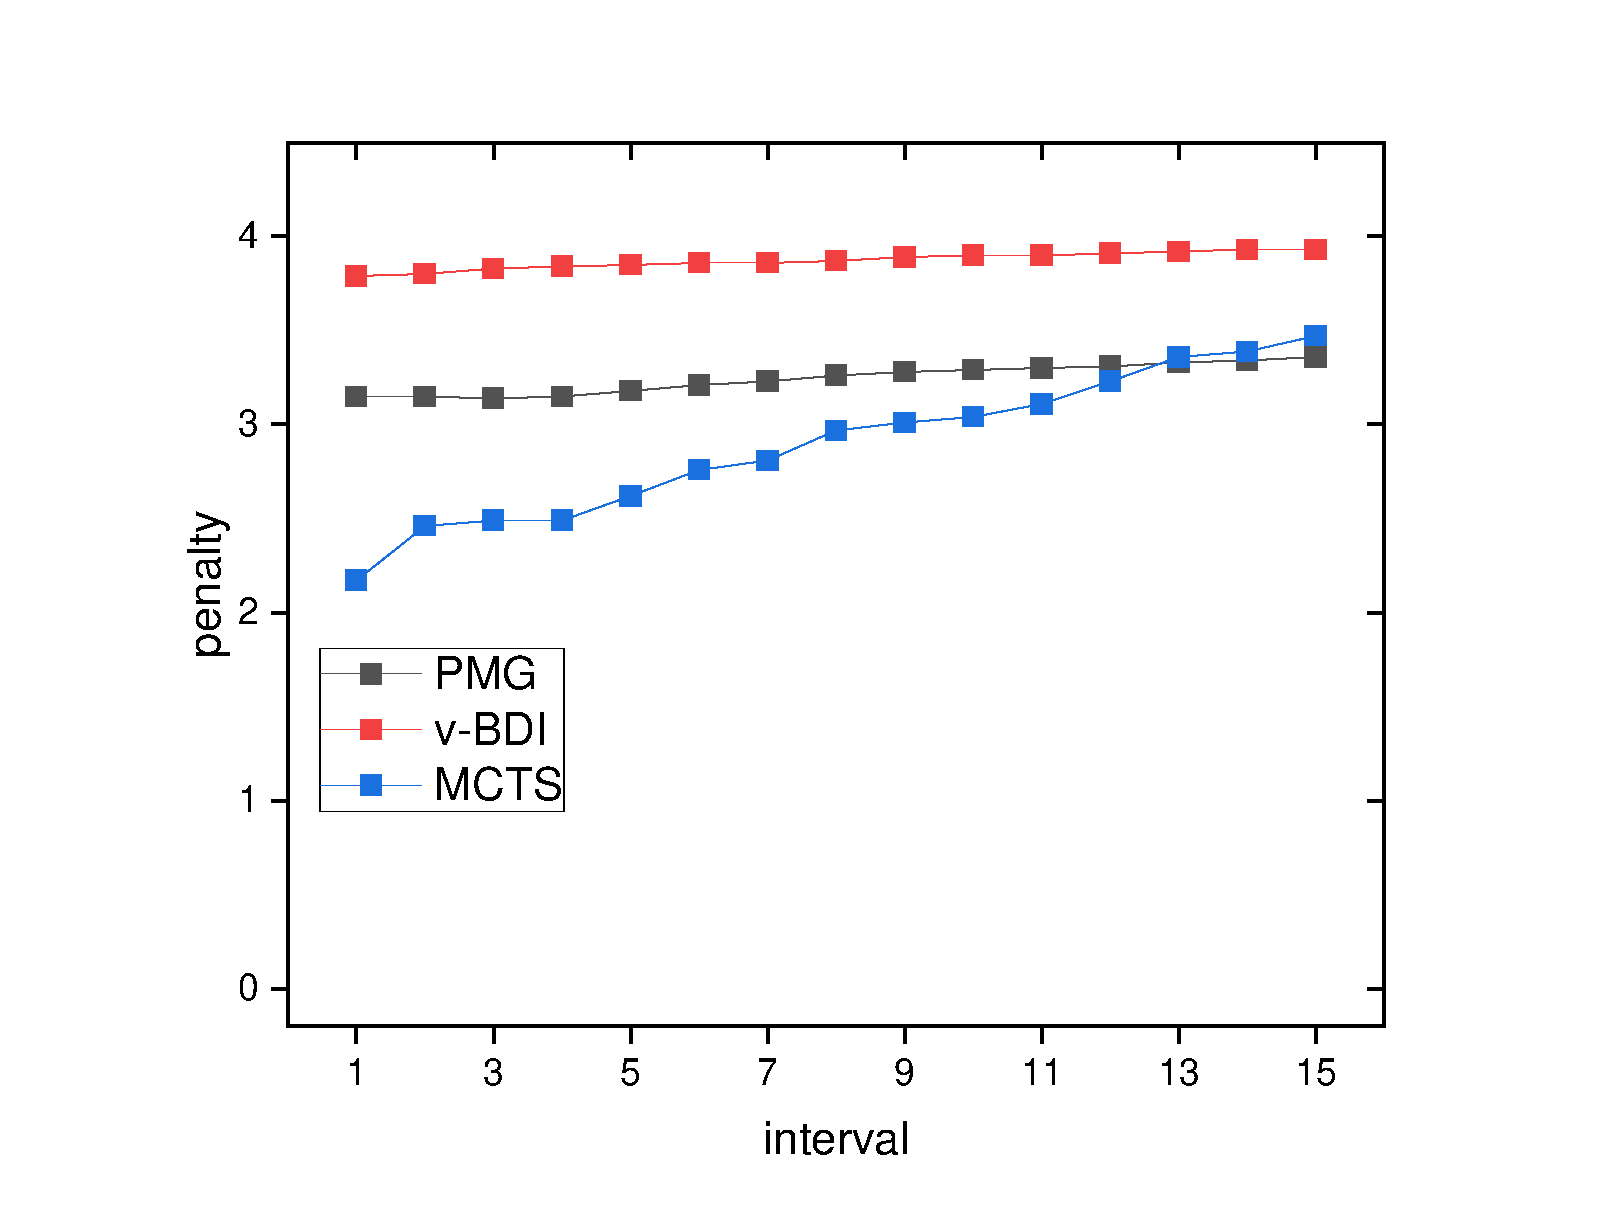
\includegraphics[scale=0.2]{inX_pY_fixCap40_simple}
  \caption{40容量}
  \captionsetup{justification=centering}
\end{subfigure}
\begin{subfigure}{.32\textwidth}
  \centering
  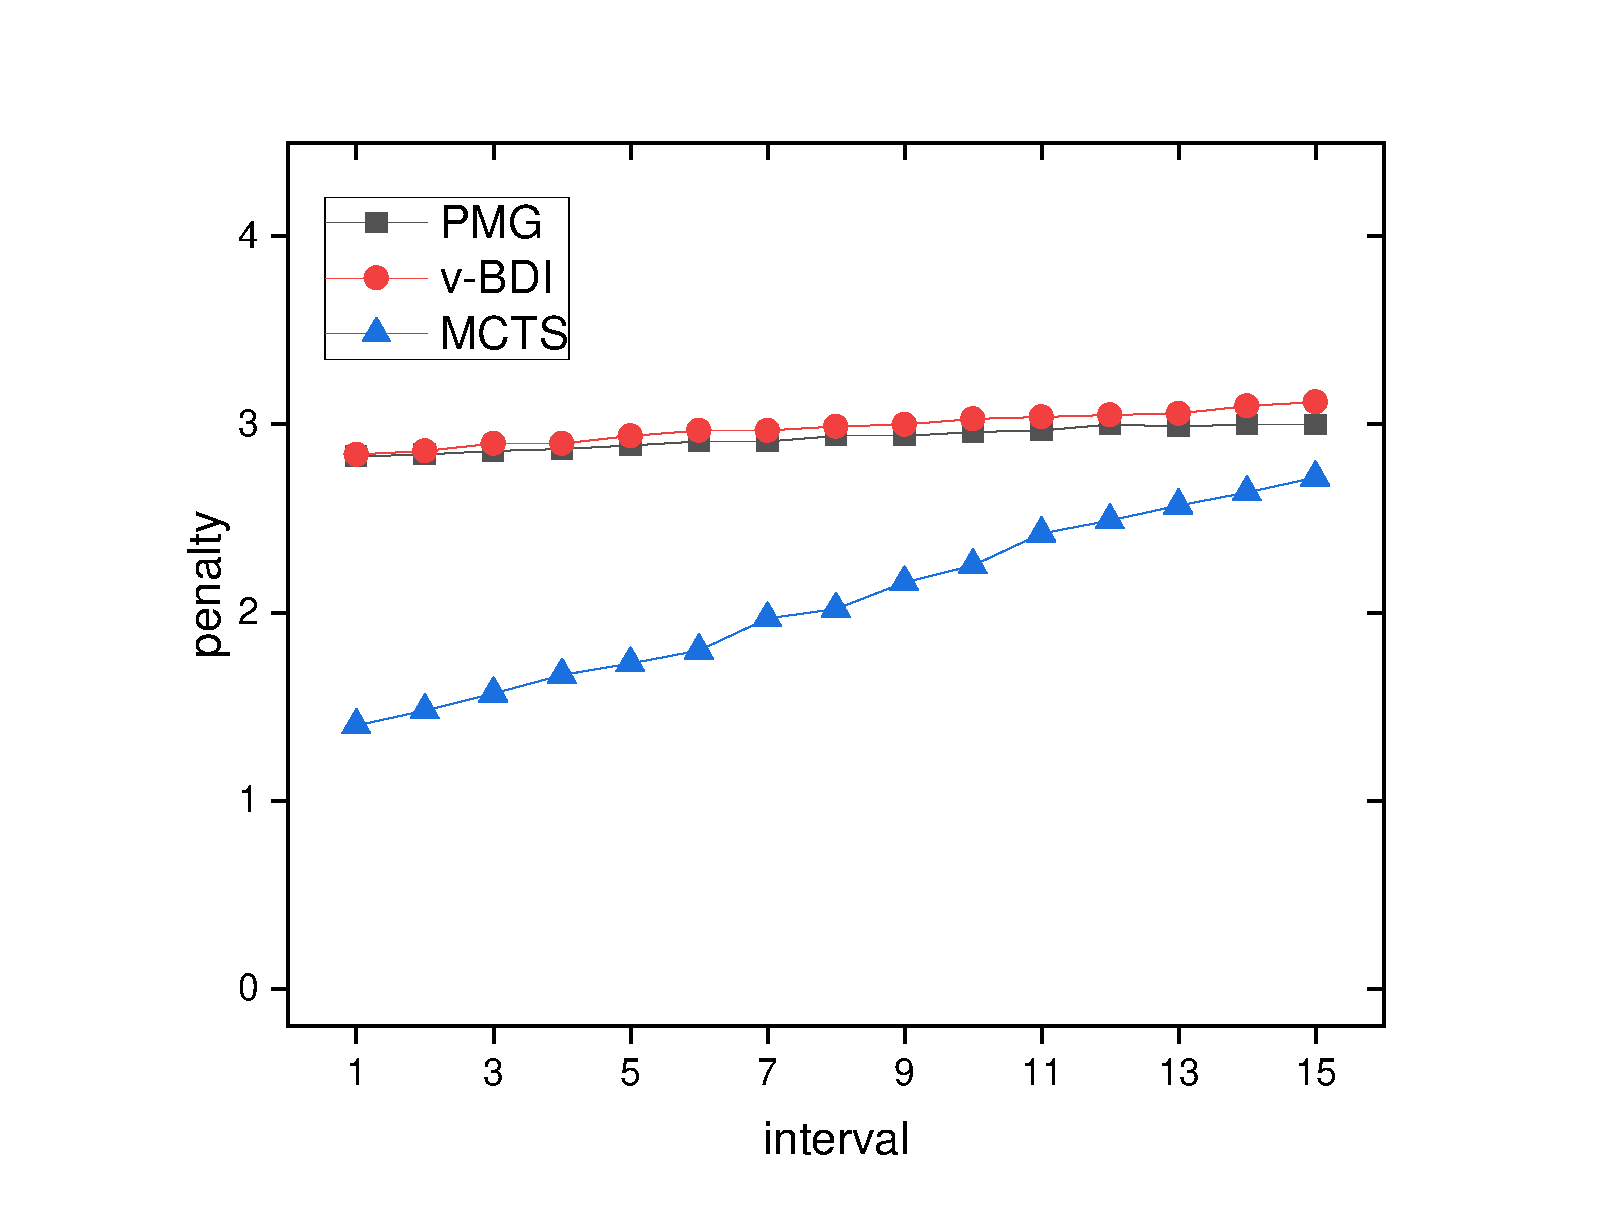
\includegraphics[scale=0.2]{inX_pY_fixCap60_simple}
  \caption{60容量}
  \captionsetup{justification=centering}
\end{subfigure}
\begin{subfigure}{.32\textwidth}
  \centering
  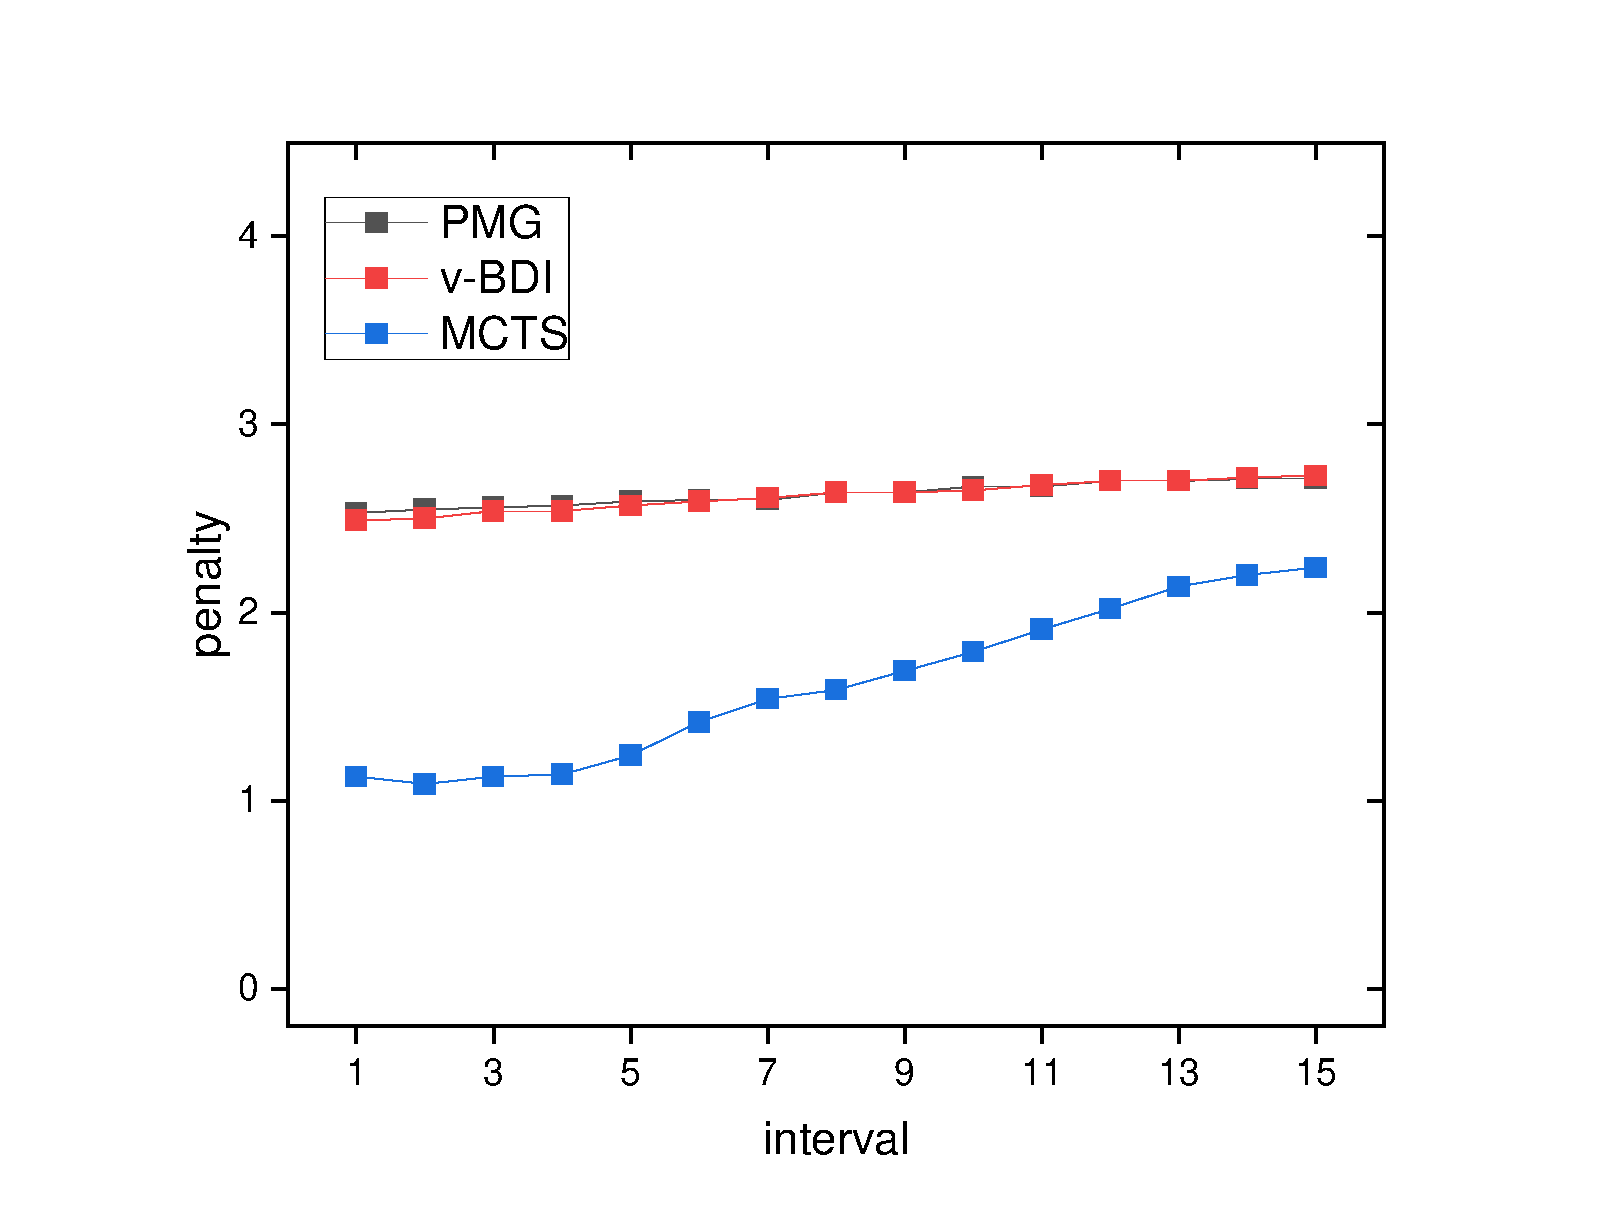
\includegraphics[scale=0.2]{inX_pY_fixCap140_simple}
  \caption{140容量}
  \captionsetup{justification=centering}
\end{subfigure}
\begin{subfigure}{.32\textwidth}
  \centering
  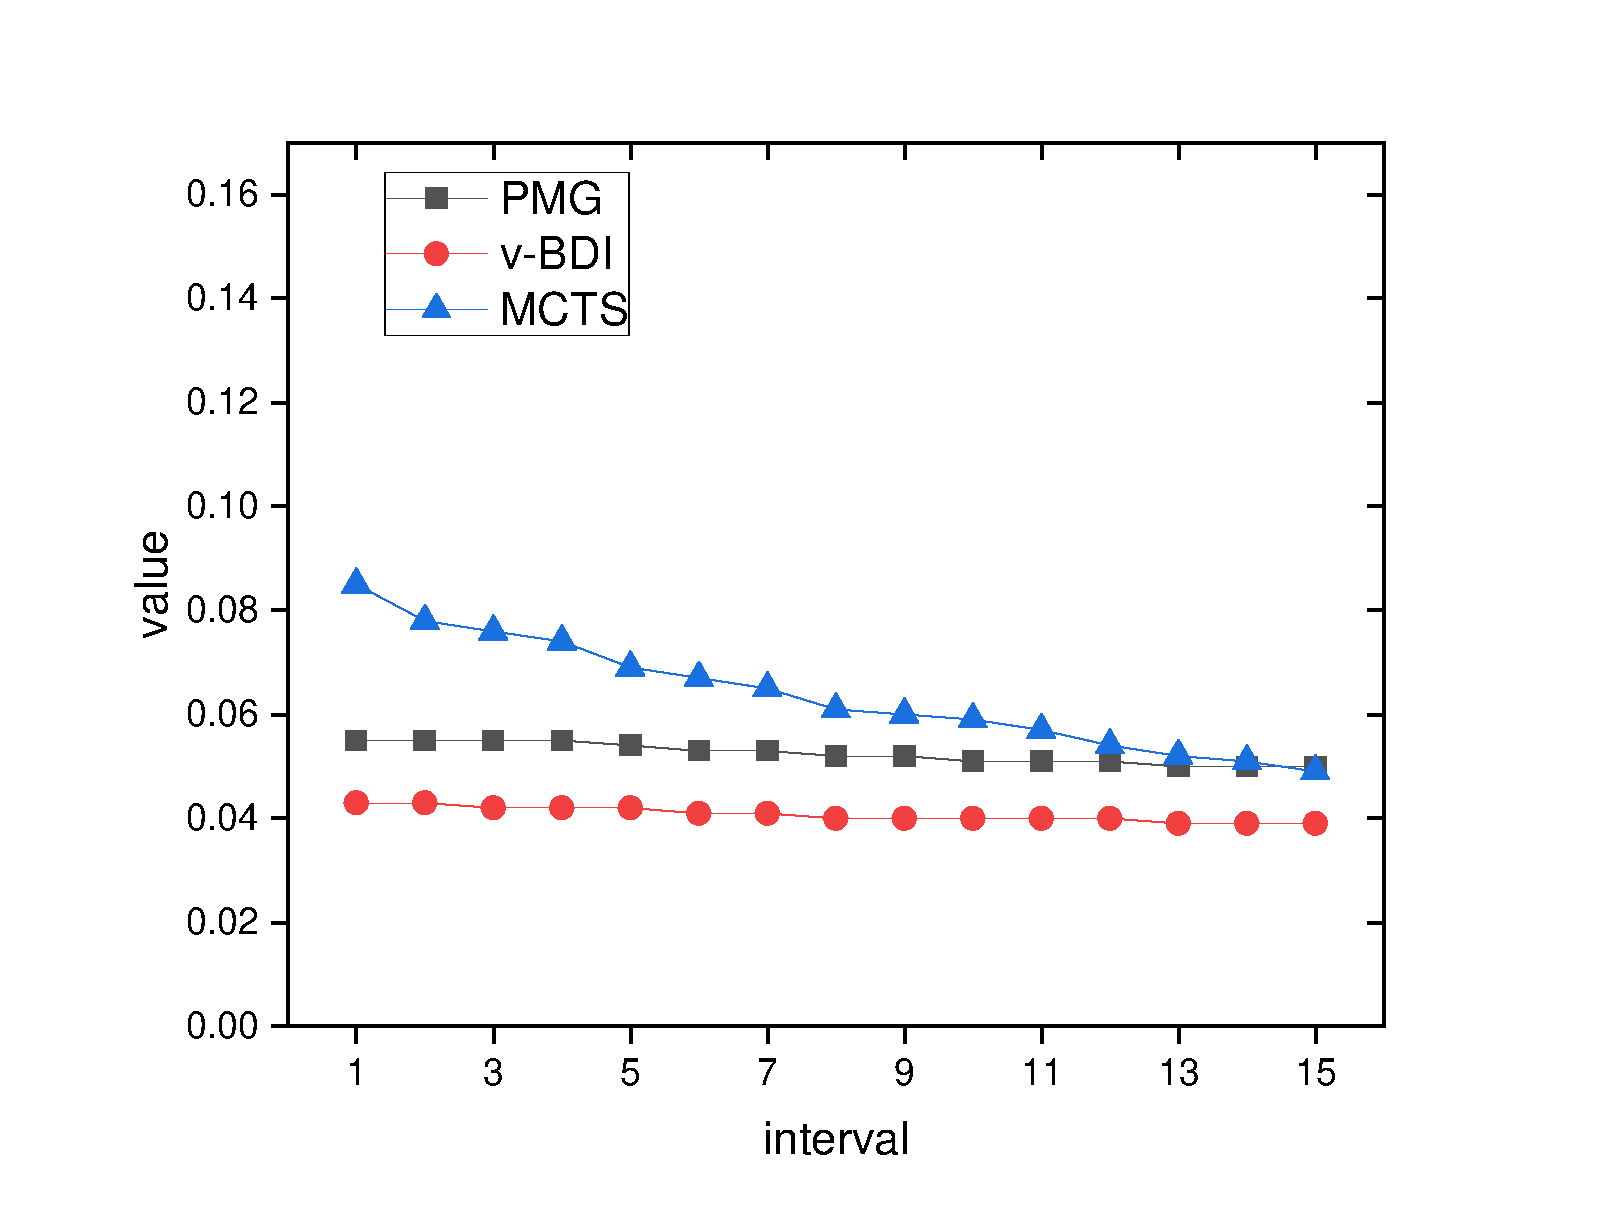
\includegraphics[scale=0.2]{inX_vY_fixCap40_simple}
  \caption{40容量}
  \captionsetup{justification=centering}
\end{subfigure}
\begin{subfigure}{.32\textwidth}
  \centering
  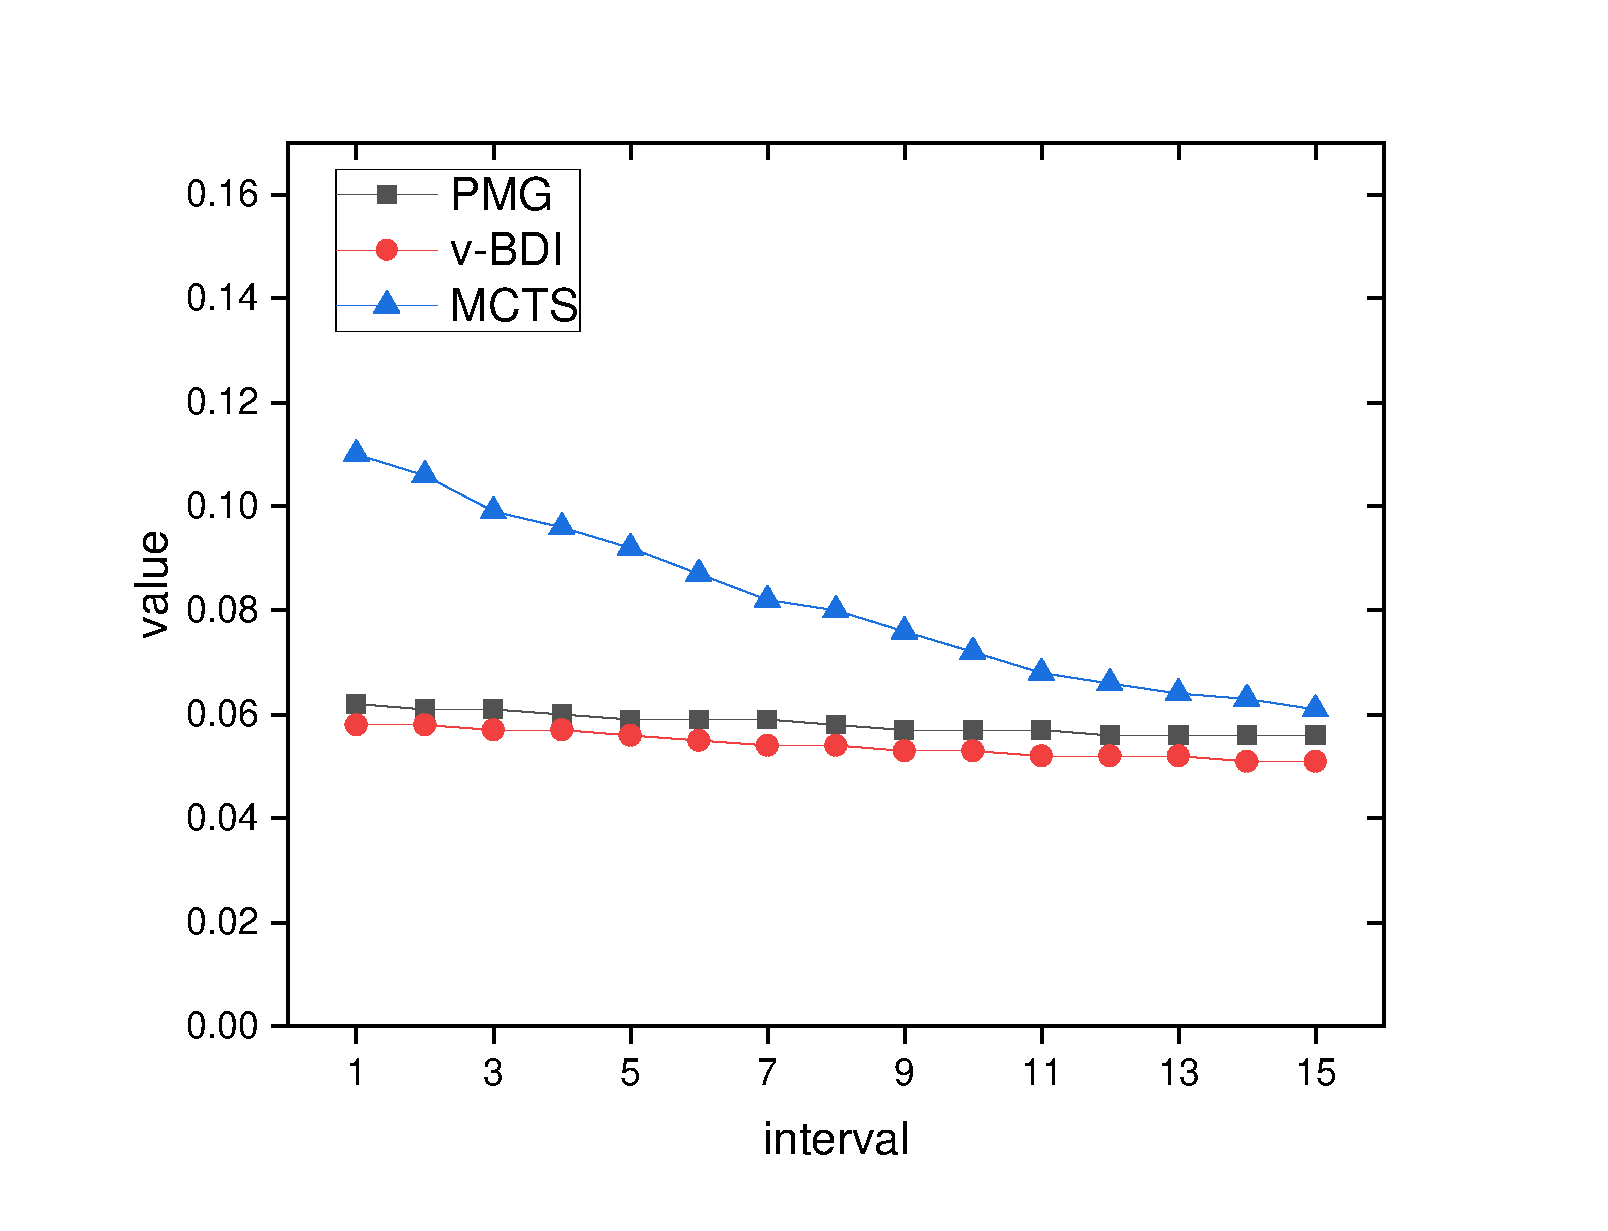
\includegraphics[scale=0.2]{inX_vY_fixCap60_simple}
  \caption{60容量}
  \captionsetup{justification=centering}
\end{subfigure}
\begin{subfigure}{.32\textwidth}
  \centering
  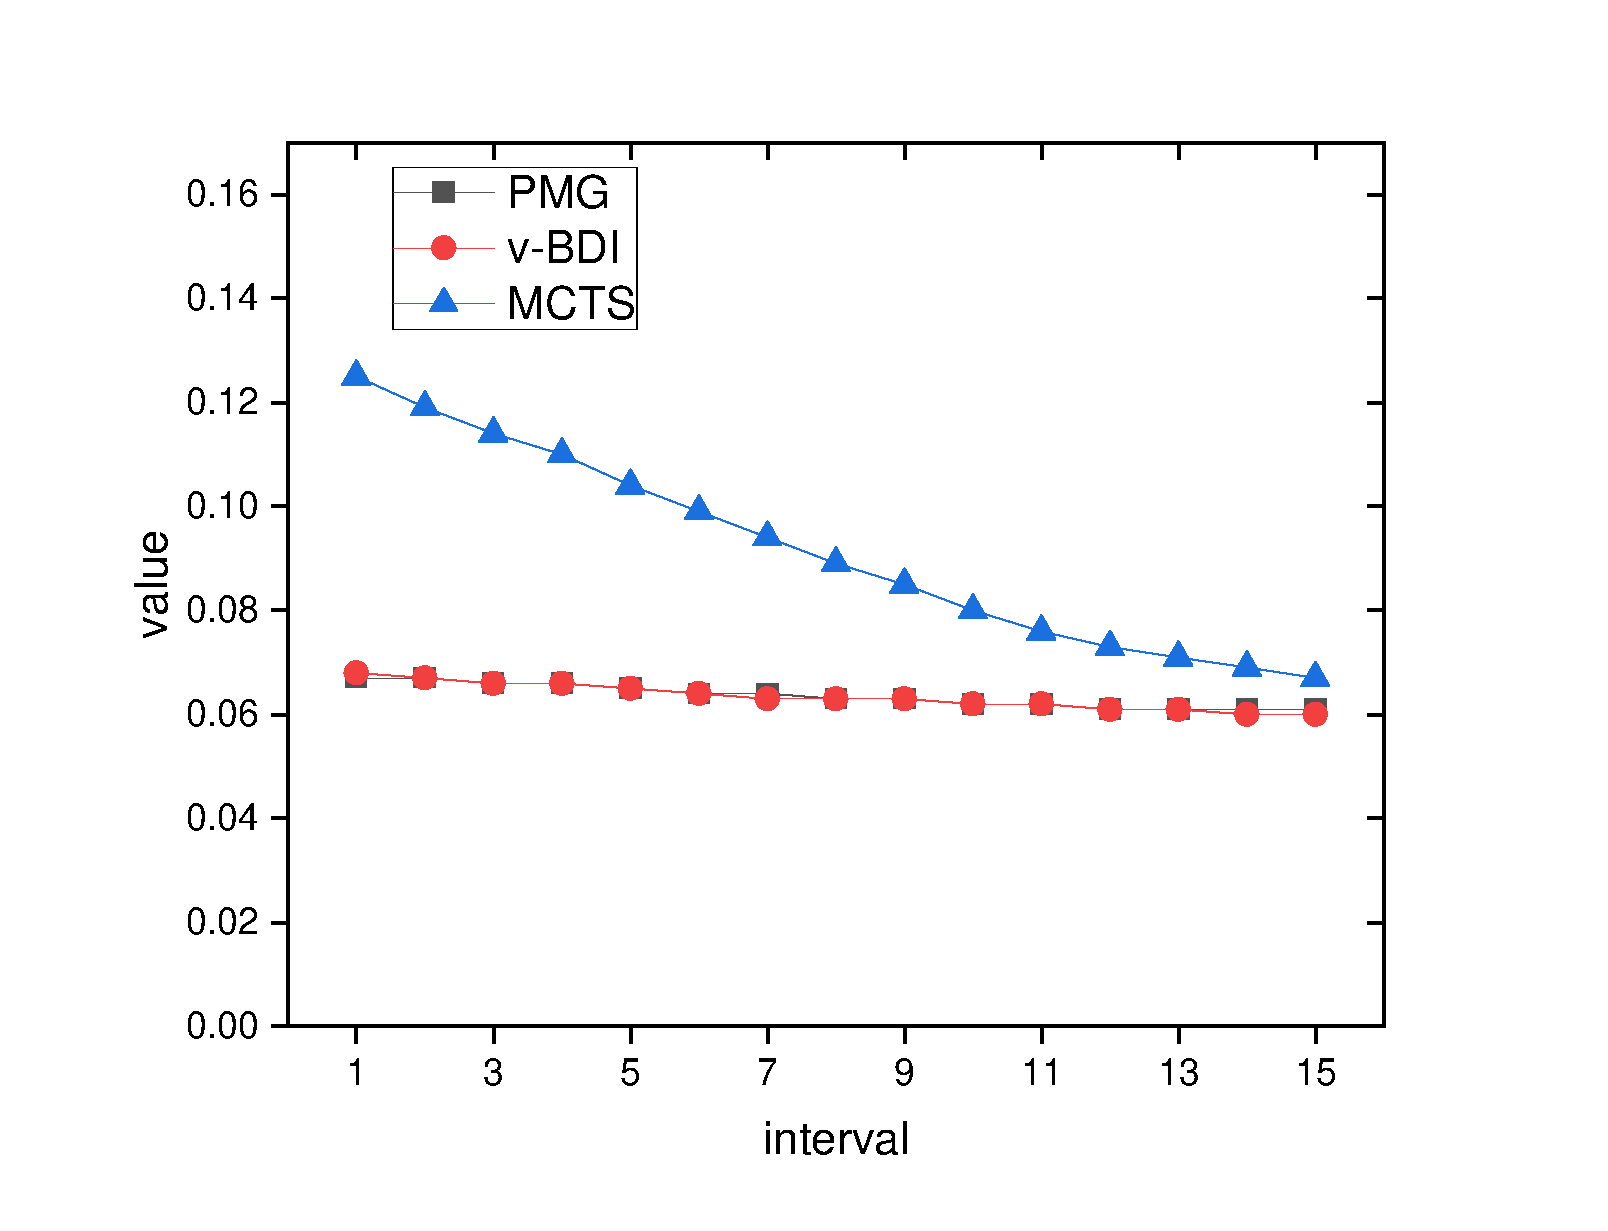
\includegraphics[scale=0.2]{inX_vY_fixCap140_simple}
  \caption{140容量}
  \captionsetup{justification=centering}
\end{subfigure}
\captionsetup{justification=centering}
\bicaption{简单地形下的动态场景实验结果}{Experiment results in dynamic simple terrain scenario}
\label{fig:dynamic_simple}
\end{figure}
从图中可以看出,在动态环境中,MCTS在大多数情况下仍然优于其他方法。然而,MCTS的优势随着时间间隔interval的增加而减少。原因是,间隔越长,智能体并行的目标就越少,这使得MCTS更难利用不同意图之间的协同作用。

\section{本章总结}
本章提出了一种基于MCTS的意图调度算法\SAT 。\SAT 可以在norm约束下同时对智能体的实现型目标和维持型目标进行意图调度。另外,基于火星探测器的模拟场景,本章在复杂地形以及简单地形场景下对\SAT 的性能进行了分析。实验结果表明\SAT 与其他方法(PMG和v-BDI)相比有着显著的性能优势。
